% LaTeX file for Chapter 03












\chapter{Results}



% \begin{table}
% 
% \caption{Comparison of confidence intervals for the mean differences across scenarios. The first row of each pair corresponds to the confidence interval from the linear model (lm), while the second row corresponds to the bootstrap method.}
% \centering
% \begin{tabular}[t]{lrr}
% \toprule
%   & Lower Bound & Upper Bound\\
% \midrule
% Scenario 1 (lm) & -0.58231 & -0.54359\\
% Scenario 1 (bootstrap) & -0.58210 & -0.54355\\
% Scenario 2 (lm) & -0.59118 & -0.55371\\
% Scenario 2 (bootstrap) & -0.59091 & -0.55405\\
% Scenario 3 (lm) & -0.06784 & -0.02799\\
% \addlinespace
% Scenario 3 (bootstrap) & -0.06784 & -0.02752\\
% \bottomrule
% \end{tabular}
% \end{table}


\section{TRAM-DAGs simple simulation study}

Intercepts: show estimates vs. dgp same as in intermediate presentation.

Show the Discrete case with just cutpints (only K-1 parameters of outputs are used)
Show the continuous case where the outputs are transformed to monotonically increasing betas for the bernstein polynomial.

Linear and complex shifts: 

Here in the first two plots we can see the linear shifts. And in the right plot we have the complex shift of X2 on X3. The estimated shifts match quite well with the DGP.

Complex shift (Interaction example) to show what is also possible:

Here I just want to make a short input from another example. So there the true model was that of a logistic regression with the binary outcome Y and 3 predictors. The binary treatment T and the two continuous predictors X1 and X2. There was also an interaction effect assumed between treatment and X1. So this basically means that the effect of X1 on the outcome is different for the two treatment groups.
And here we can show that our TRAM-DAG specified by a complex shift of T and X1 can also capture this interaction effect quite well.


\section{ITE simulation study - when do causal ML models fail?}

In this section, we present the performance of different causal ML models for estimating the ITE under different scenarios. Starting with a favourable scenario where everything is assumed to be known and effect sizes are large, we will sequentially introduce more complexity and uncertainty into the data generating process (DGP) to see how the models perform under less favourable conditions. The scenarios are designed to reflect different real-world situations, such as the presence of (confounding variables - maybe not include, since ITE estimation must assume no unobserved confounding?), interaction effects, and varying treatment effects across individuals and unobserved variables.

The results are presented for all causal ML models per scenario.

In each scenario we present the results of the simple model (glm tlearner, basically dgp) and a complex model (tuned random forest). In the appendix, the results in scenario 1 of a not-tuned random forest are presented as an example that it is crucial to tune the model so that it is appropriate for ITE (and in this case probability calculation) estimation, hence well calibrated.


\subsection{Scenario (1): Fully observed, large effects}


\begin{figure}[htbp]
\centering
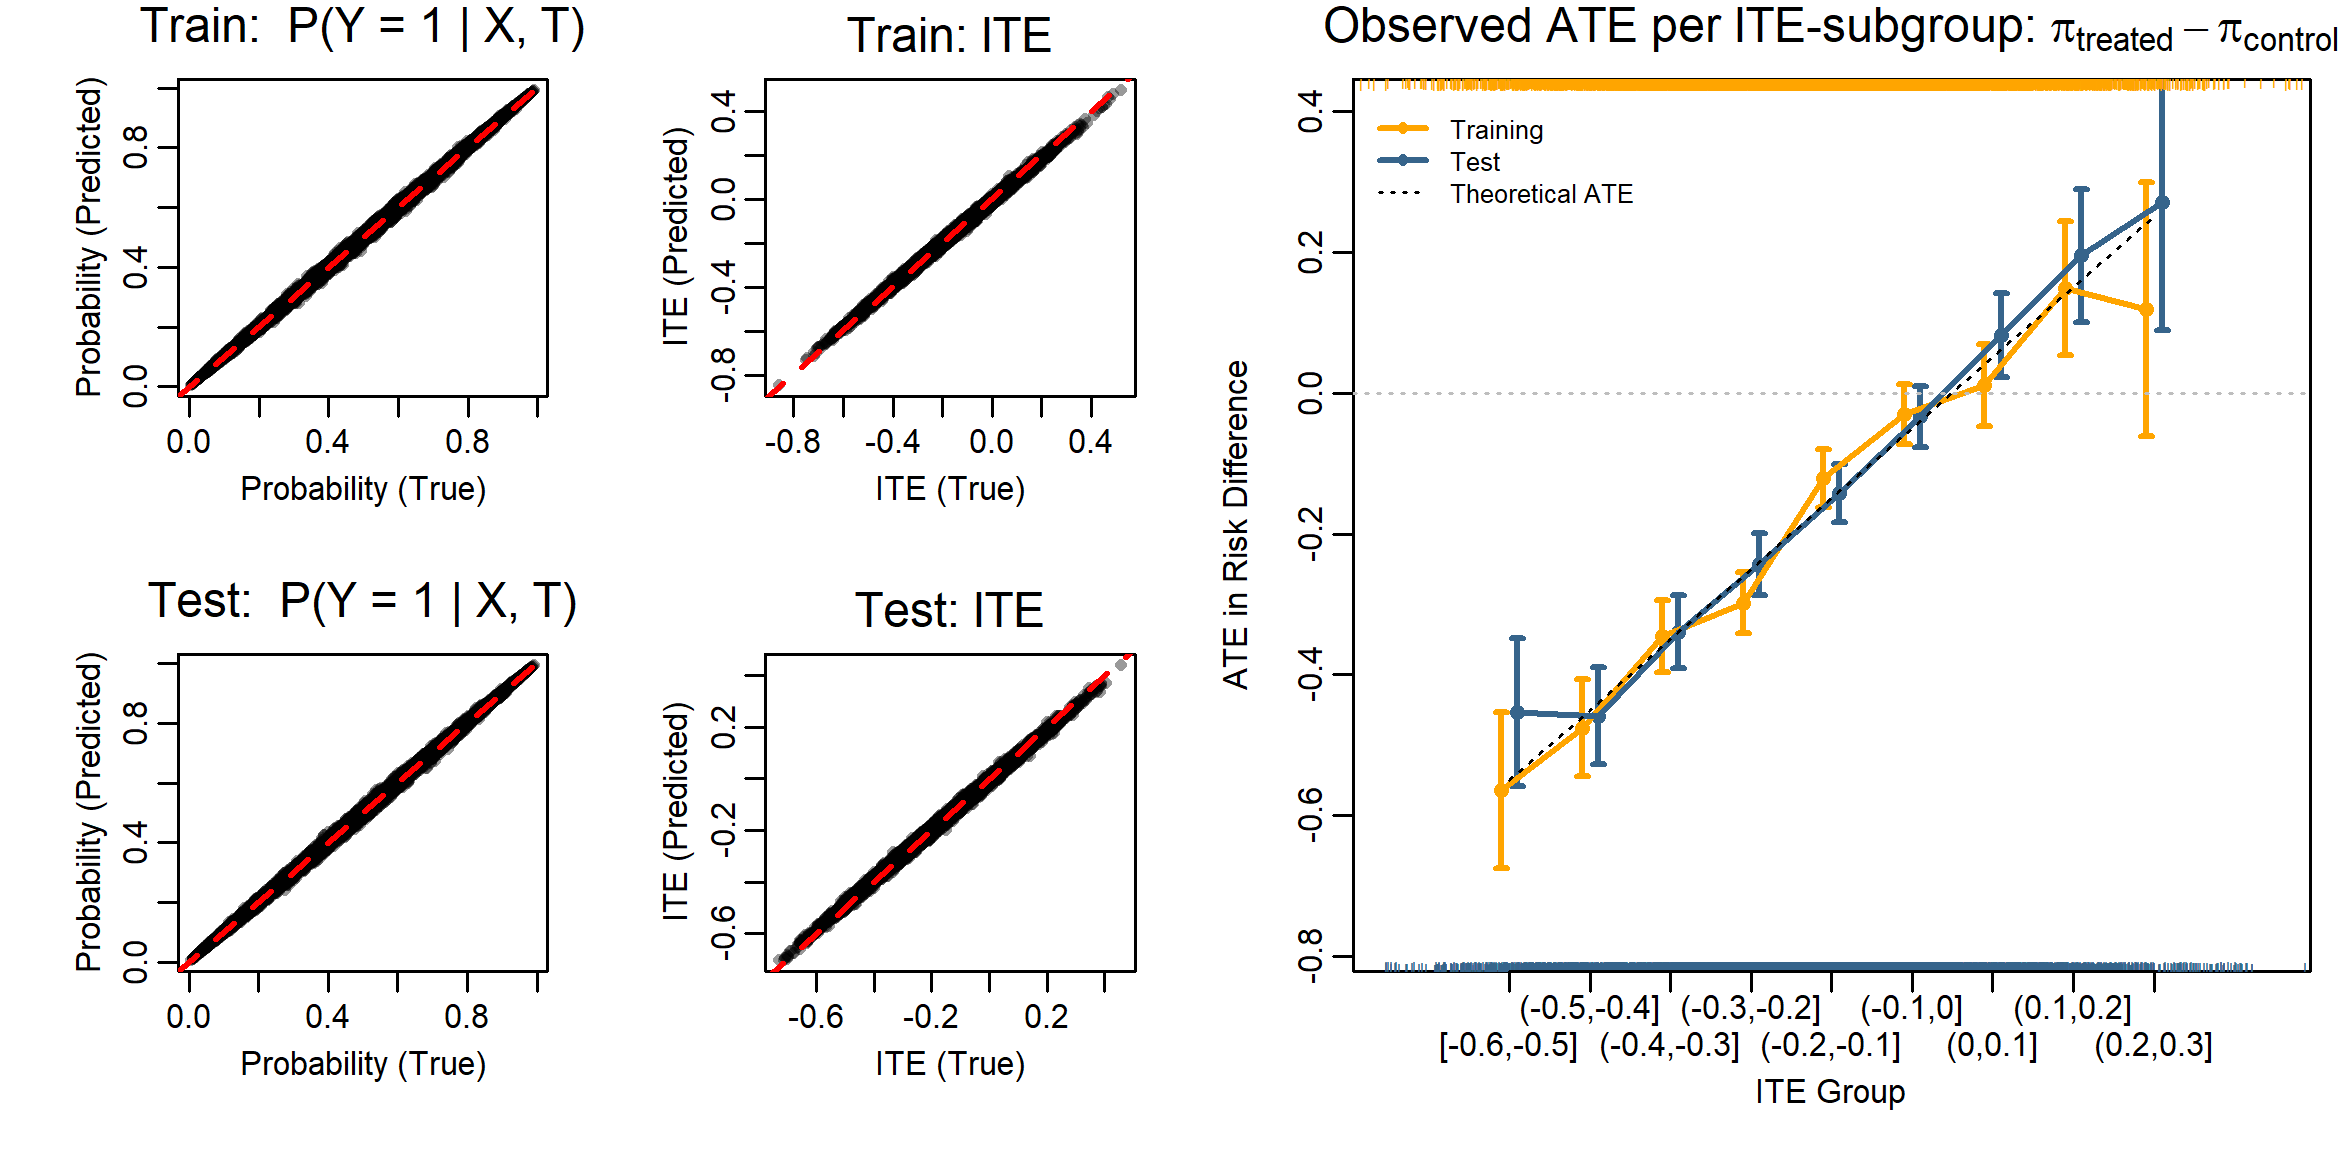
\includegraphics[width=0.9\textwidth]{img/results_ITE_simulation/fully_observed_glm_tlearner.png}
\caption{Results with the GLM T-learner when the DAG is fully observed, strong effects.}
\label{fig:fully_observed_glm_tlearner}
\end{figure}


\begin{figure}[htbp]
\centering
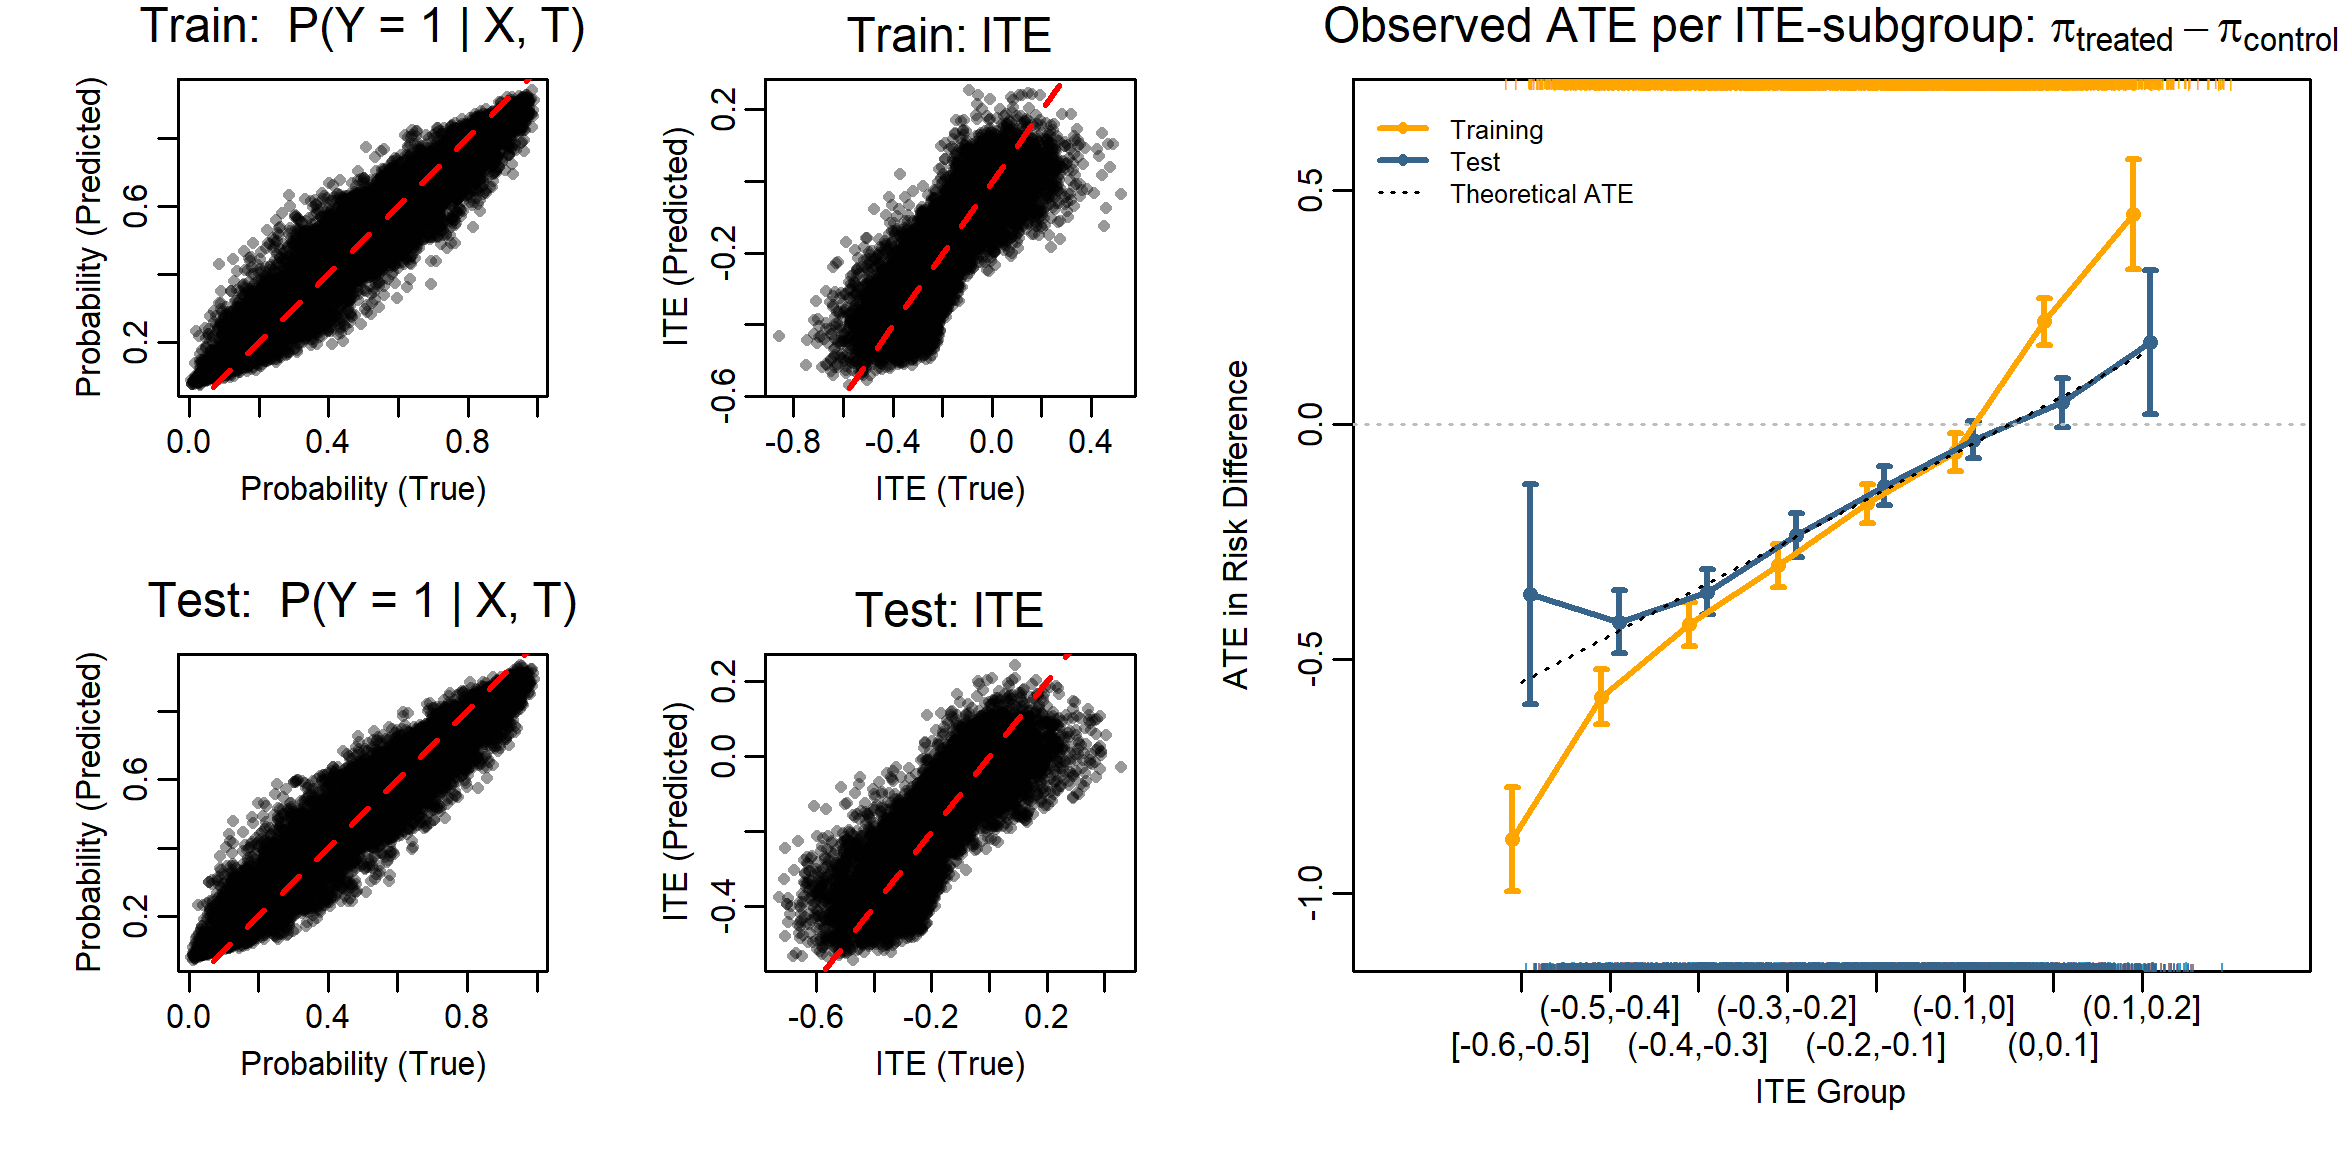
\includegraphics[width=0.9\textwidth]{img/results_ITE_simulation/fully_observed_tuned_rf_tlearner.png}
\caption{Results with the Tuned Random Forest (comets) T-learner when the DAG is fully observed, strong effects.}
\label{fig:fully_observed_glm_tlearner}
\end{figure}




\subsection{Scenario (2): unobserved interaction}


\begin{figure}[htbp]
\centering
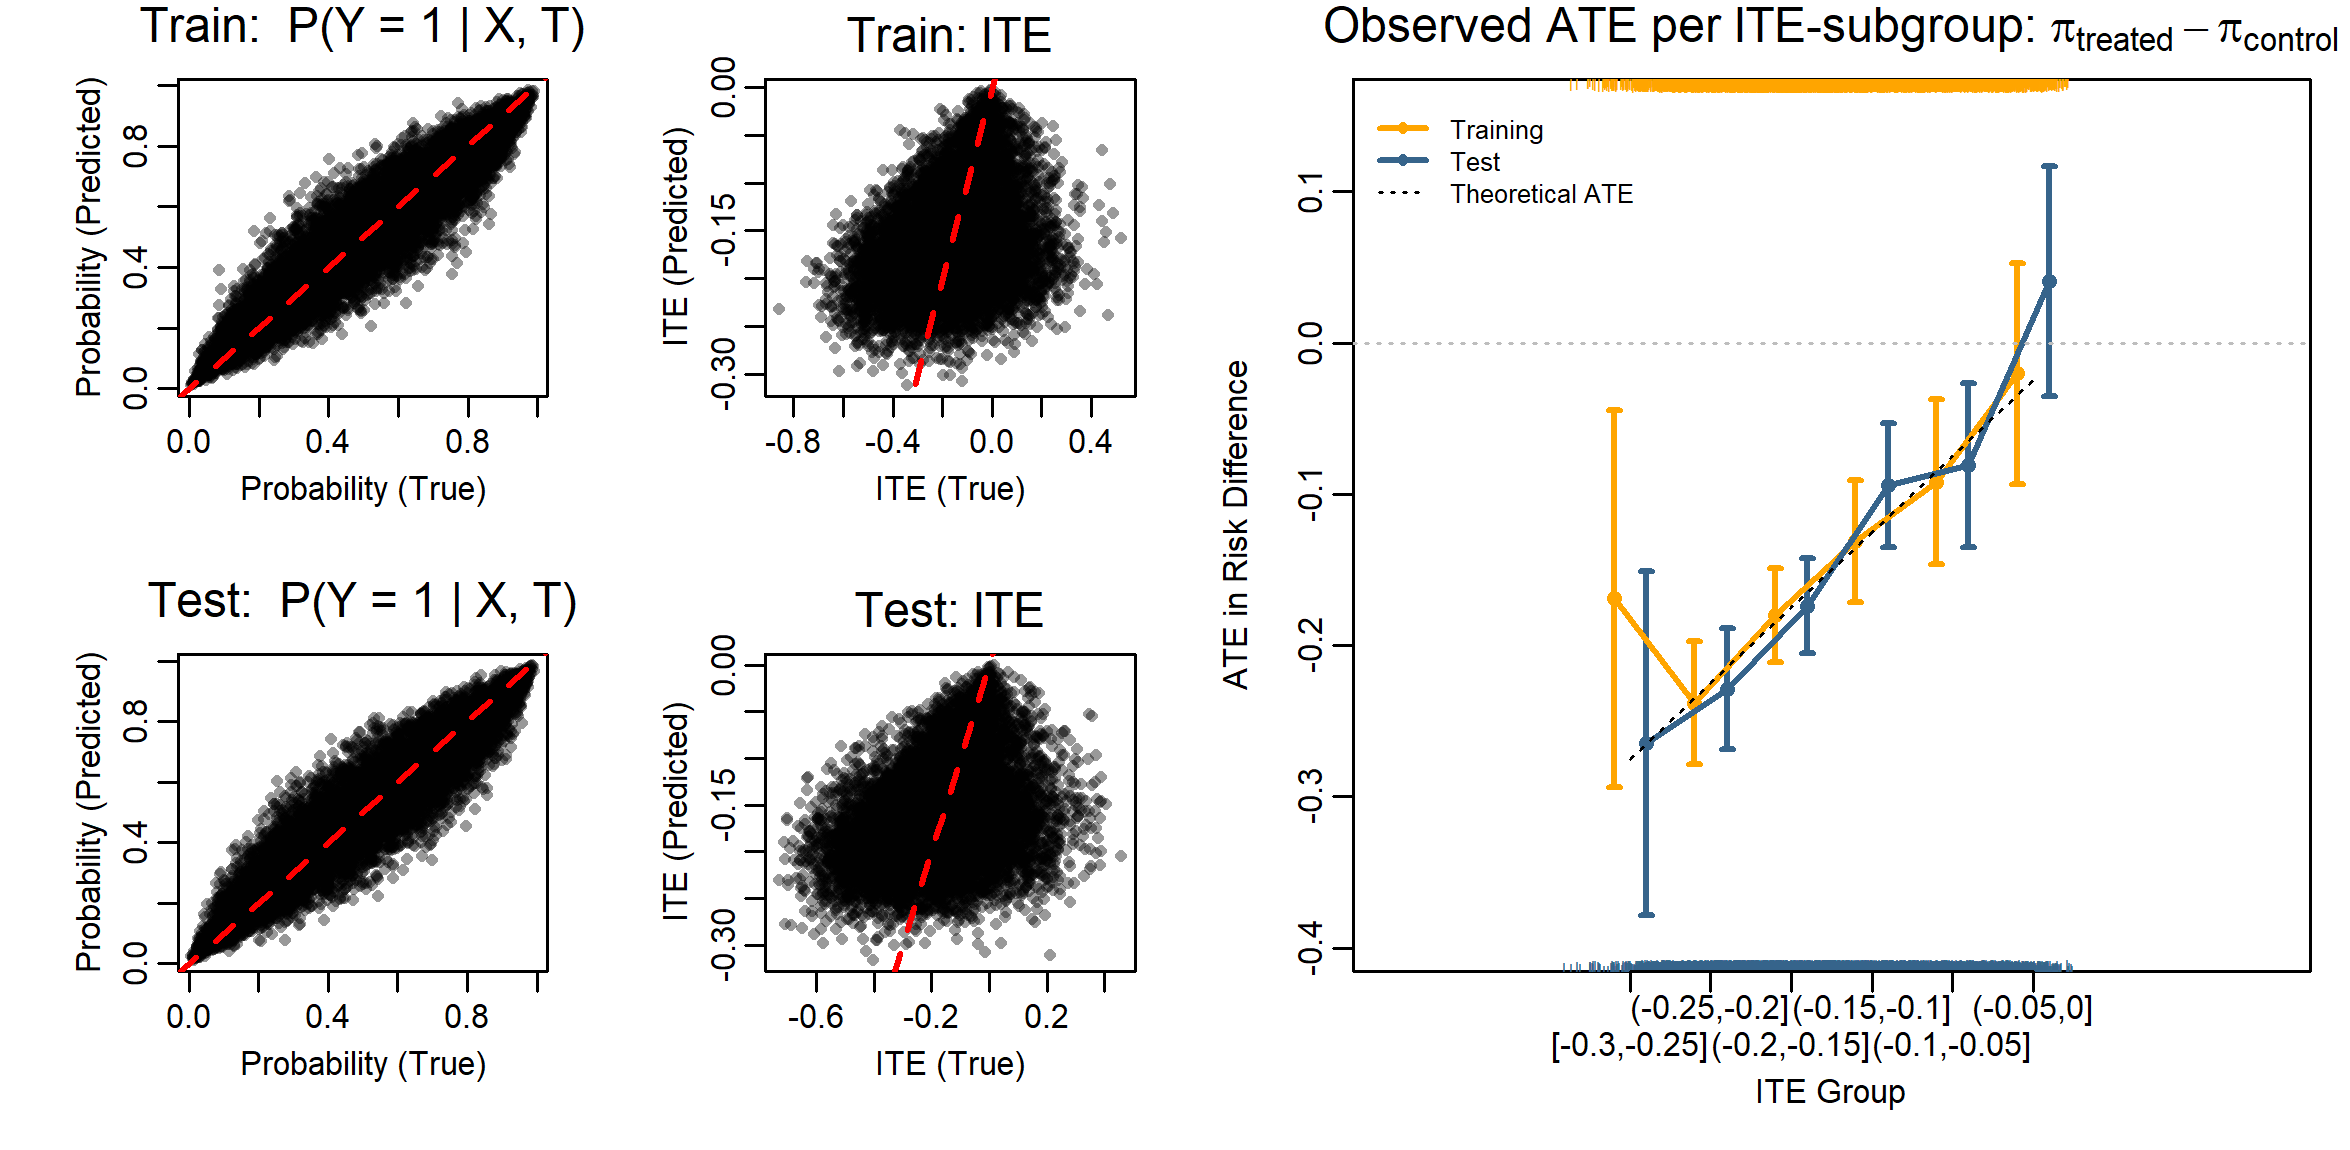
\includegraphics[width=0.9\textwidth]{img/results_ITE_simulation/unobserved_interaction_glm_tlearner.png}
\caption{Results with the GLM T-learner if the interaction variable is unobserved, strong effects.}
\label{fig:unobserved_interaction_glm_tlearner}
\end{figure}


\begin{figure}[htbp]
\centering
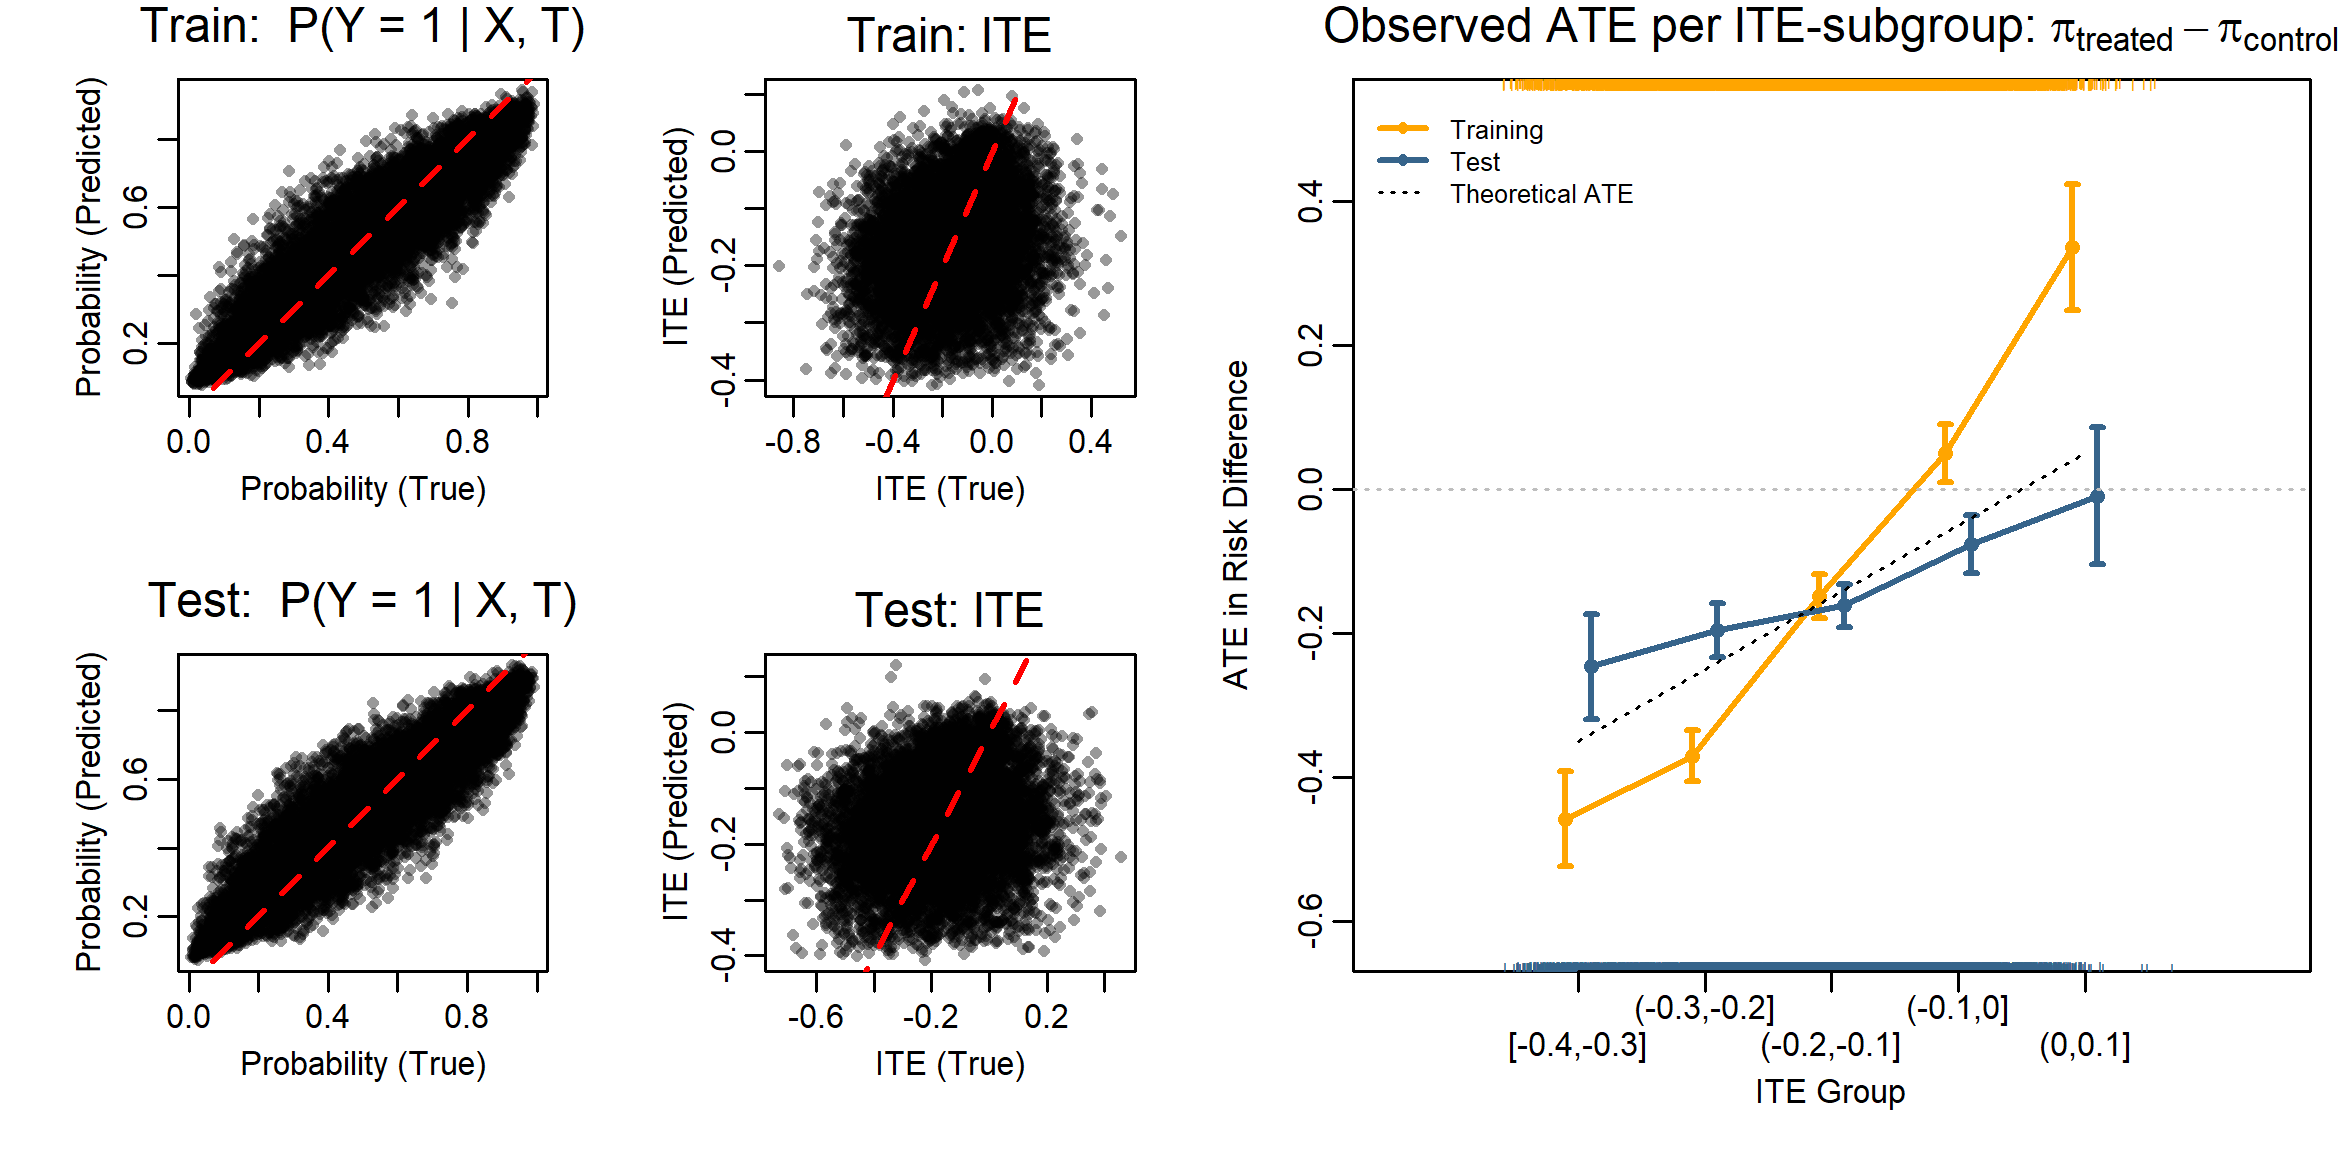
\includegraphics[width=0.9\textwidth]{img/results_ITE_simulation/unobserved_interaction_tuned_rf_tlearner.png}
\caption{Results with the Tuned Random Forest (comets) T-learner if the interaction variable is unobserved, strong effects.}
\label{fig:unobserved_interaction_glm_tlearner}
\end{figure}


\section{ITE estimation with TRAM-DAGs}

First, we present the results for scenario (1) with a direct and interaction effect. Then, we present the results for scenario (2) with a direct effect but no interaction effects, and finally, scenario (3) with interaction effects but no direct effect of the treatment. For each scenario, we compare the results in an observational setting with confounded treatment allocation and in a randomized controlled trial (RCT) setting without confounders. We also compare the average treatment effect (ATE), which can directly be calculated in the RCT, with the ATE based on the estimated individualized treatment effects. If the estimated ITEs are unbiased, they should be a good estimate of the ATE. All ITEs presented in this section are technically quantile treatment effects (QTEs) based on the 0.5-quantile of the potential outcomes. For simplicity we will refer to them as ITEs in the following.


\subsection{Scenario (1): Direct and interaction effects}

Scenario (1) included a direct effect of the treatment on the outcome and an additional interaction effect of the treatment with the covariates X2 and X3. A train and test set were generated with 20'000 observations each. In the observational setting, the treatment allocation was confounded by the covariates X1 and X2.  In the train set, $38.6$\% of patients were in the control group and $61.4$\% were in the treatment group. This ratio was similar in the test set. In the RCT setting treatment allocation was randomized. In the train set $49.8$\% individuals were in the control group and $50.2$\% in the treatment group. In the test set $50.2$\% were in the control group and $49.8$\% in the treatment group. Figure \ref{fig:scenario1_ite_distribution_dgp} illustrates the true ITE distribution that resulted from the DGP. Due to the interaction effects, there is some heterogeneity in the ITE distribution. Figure \ref{fig:scenario1_sampling_distributions_vertical} shows the marginal distributions of all variables according to the DGP and the estimates of the fitted TRAM-DAG. Figure \ref{fig:scenario1_outcome_distributions} shows the distribution of the outcome under the do(Tr=0) and do(Tr=1) interventions. The fitted model was applied to estimate the ITEs in terms of the difference in medians of the potential outcomes. The resulting density of the estimated ITEs compared to the true ITEs according to the DGP is shown in Figure \ref{fig:scenario1_ite_densities_train_test}. Across both settings, the densities of the estimated ITEs are close to the true densities in both the training and test datasets. Figure \ref{fig:scenario1_ite_scatter_train_test} shows the scatterplots of true against estimated ITEs. Finally, Figure \ref{fig:scenario1_ite_cATE} displays the ITE-ATE plot where the ATE is computed as the difference in medians of the observed outcome under the treatments within the respective ITE-subgroups The trends observed in the training and test sets are consistent.

The average treatment effect (ATE) is presented in Table \ref{tab:scenario1_ate_comparison}. In the RCT setting in the training set, the difference in means of the outcomes in the two treatment groups was $-0.563$ with a confidence interval of $-0.582$ to $-0.543$. The ATE in terms of the difference in medians of the observed outcomes was $-0.626$. Also in the training set, the ATE in terms of the mean of the true ITEs was $-0.62$ and the ATE in terms of the mean of the estimated ITEs was $-0.619$. All measures, including the ones from the test datasets, are shown in Table \ref{tab:scenario1_ate_comparison}.

NOTE: also add CIs in the table with the ATEs?

\begin{table}[htbp]
\centering
\small
\caption{Scenario (1), including direct and interaction effects: Comparison of ATE measures across train and test sets for the observational and RCT setting.}
\label{tab:scenario1_ate_comparison}
\begin{tabular}{l c c c c}
\toprule
\textbf{Measure} & \multicolumn{2}{c}{\textbf{Observational}} & \multicolumn{2}{c}{\textbf{RCT}} \\
\cmidrule(lr){2-3} \cmidrule(lr){4-5}
 & \textbf{Train} & \textbf{Test} & \textbf{Train} & \textbf{Test} \\
\midrule
ATE as $\text{mean}(\text{Y}_\text{observed}^{(1)}) - \text{mean}(\text{Y}_\text{observed}^{(0)})$ & NA & NA & -0.563 & -0.563 \\
ATE as $\text{median}(\text{Y}_\text{observed}^{(1)}) - \text{median}(\text{Y}_\text{observed}^{(0)})$  & NA & NA & -0.626 & -0.638 \\
ATE as mean(ITE$_\text{true}$)  & -0.62 & -0.622 & -0.62 & -0.622 \\
ATE as mean(ITE$_\text{estimated}$) & -0.617 & -0.62 & -0.619 & -0.622 \\
\bottomrule
\end{tabular}
\end{table}




\begin{figure}[htbp]
\centering
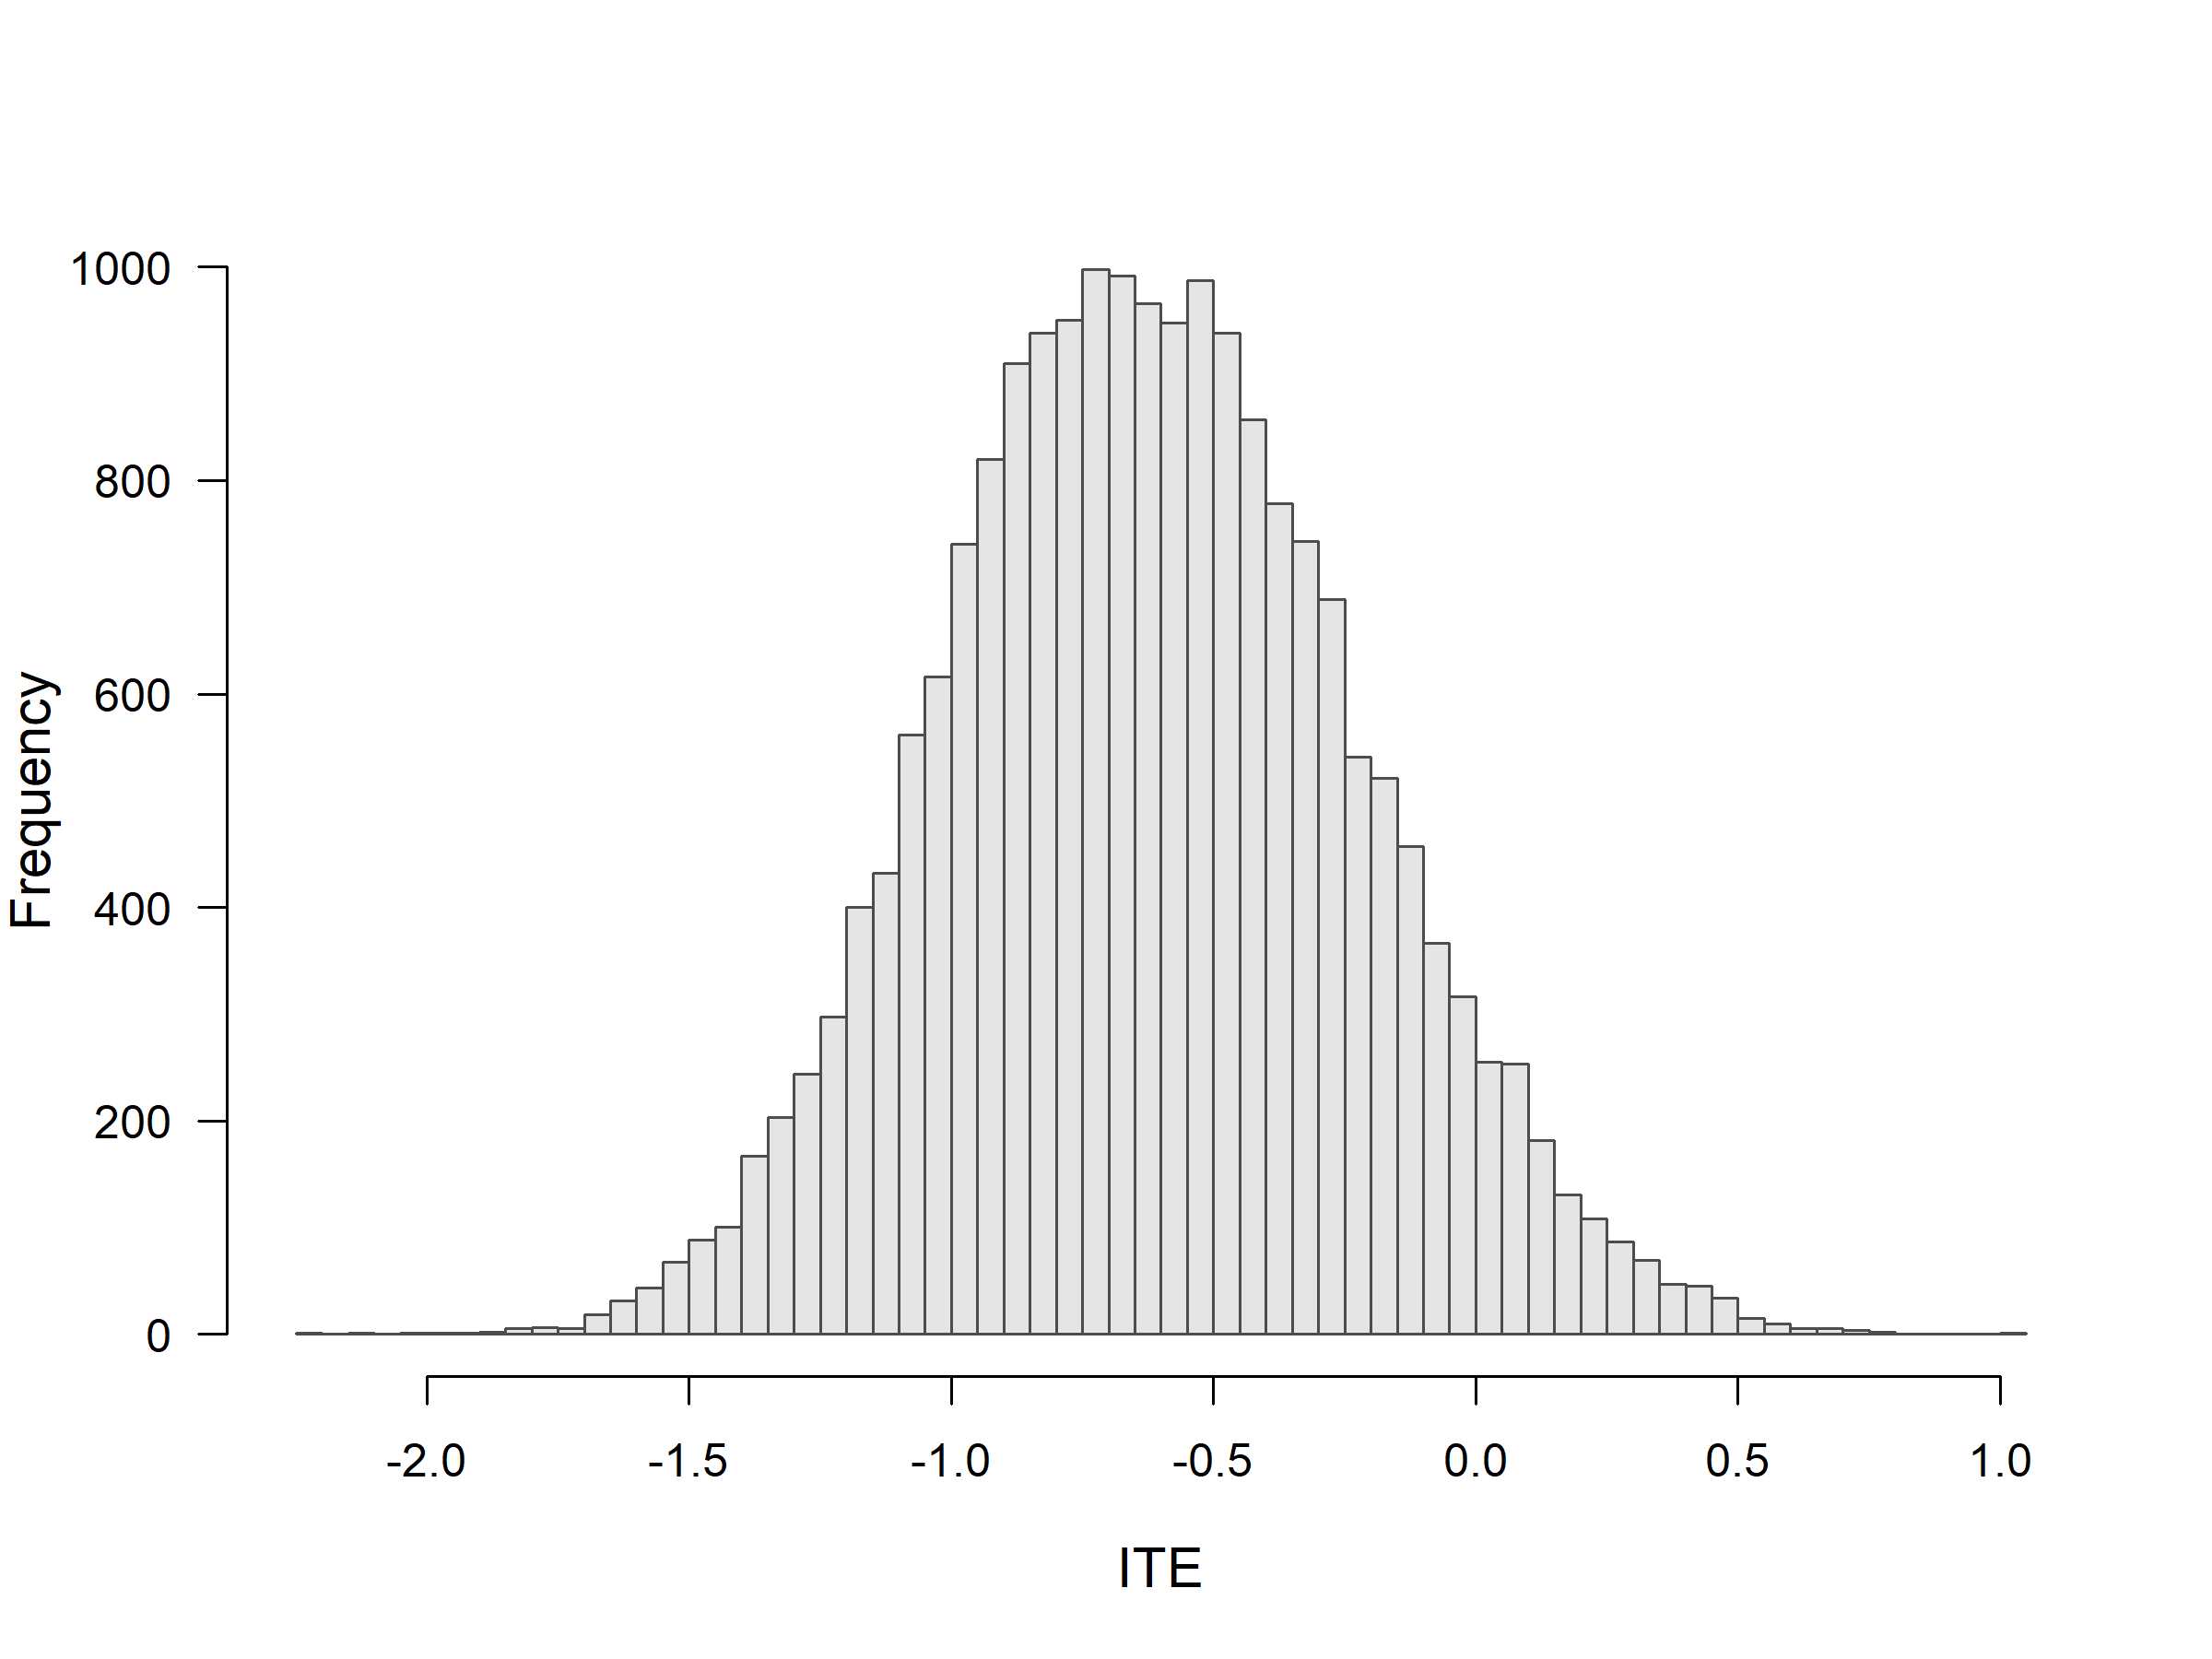
\includegraphics[width=0.45\textwidth]{img/results/observ_scenario1_ite_distribution_dgp.png}
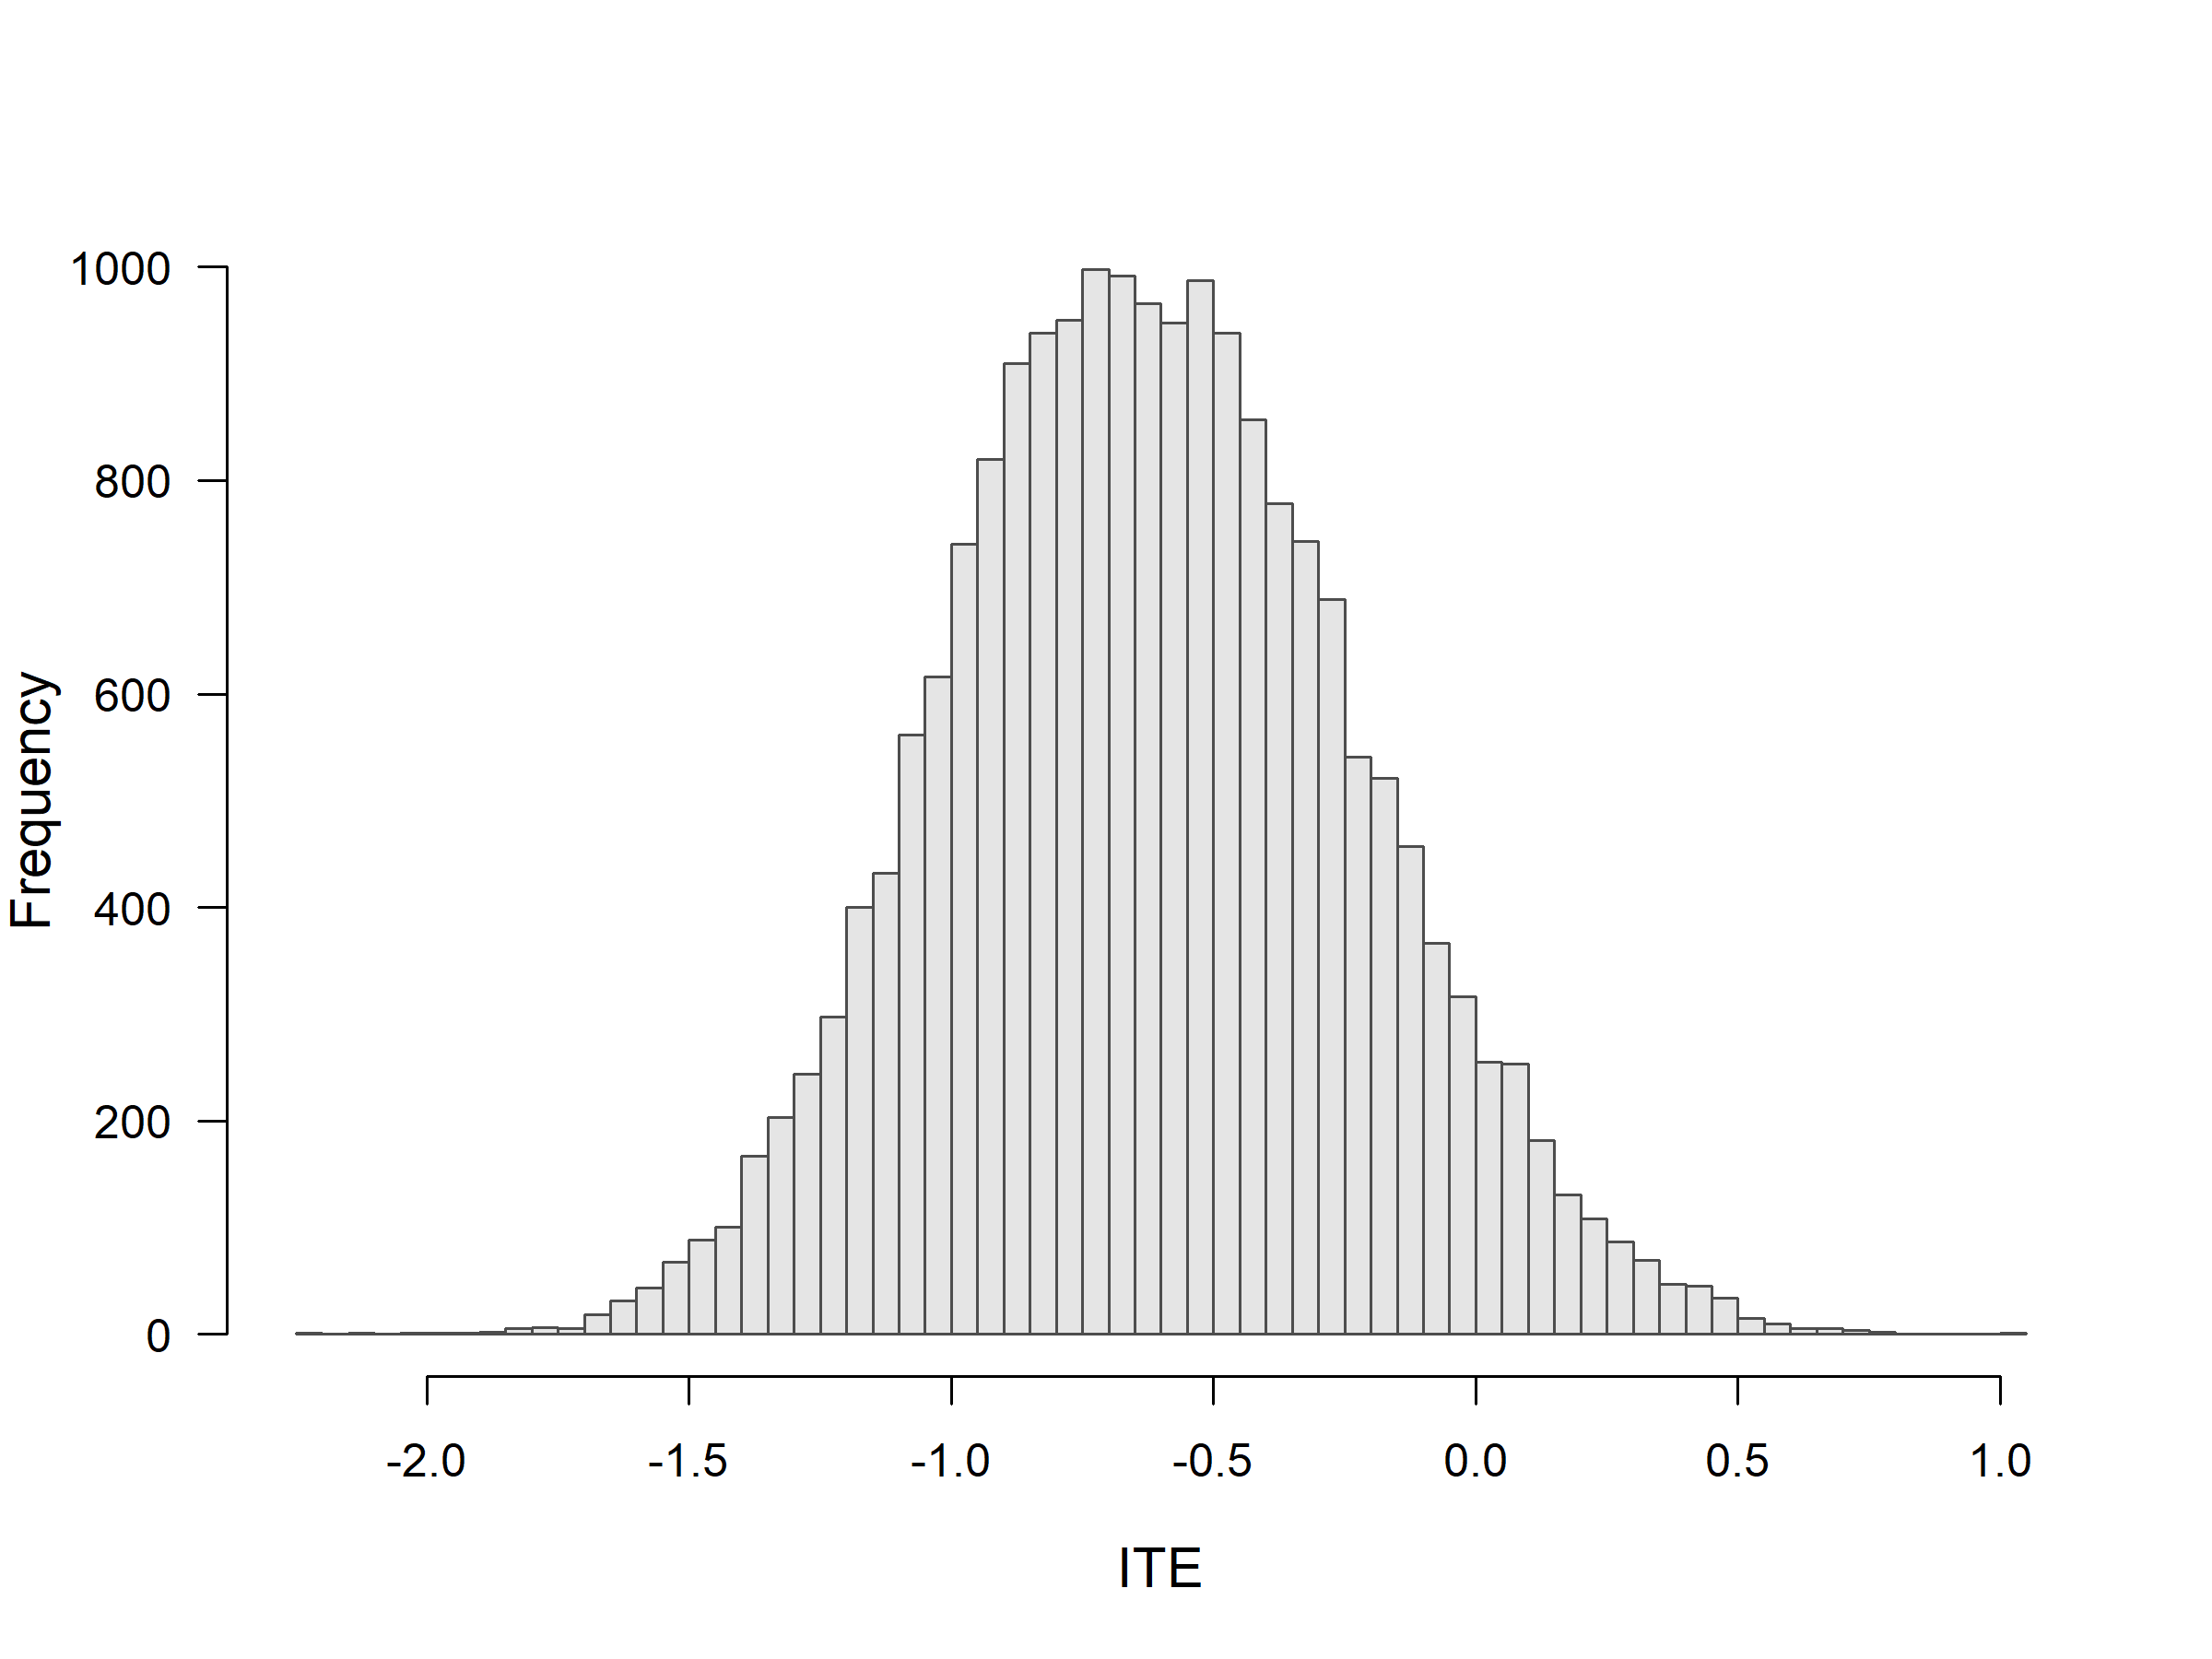
\includegraphics[width=0.45\textwidth]{img/results/rct_scenario1_ite_distribution_dgp.png}
\caption{True ITE distribution resulting from the DGP for scenario (1) with direct and interaction effects. The true ITEs are identical in the observational and in the RCT setting, since they depend on the potential outcomes under both treatment allocations. Left: Observational; Right: RCT setting.}
\label{fig:scenario1_ite_distribution_dgp}
\end{figure}



\begin{figure}[htbp]
\centering
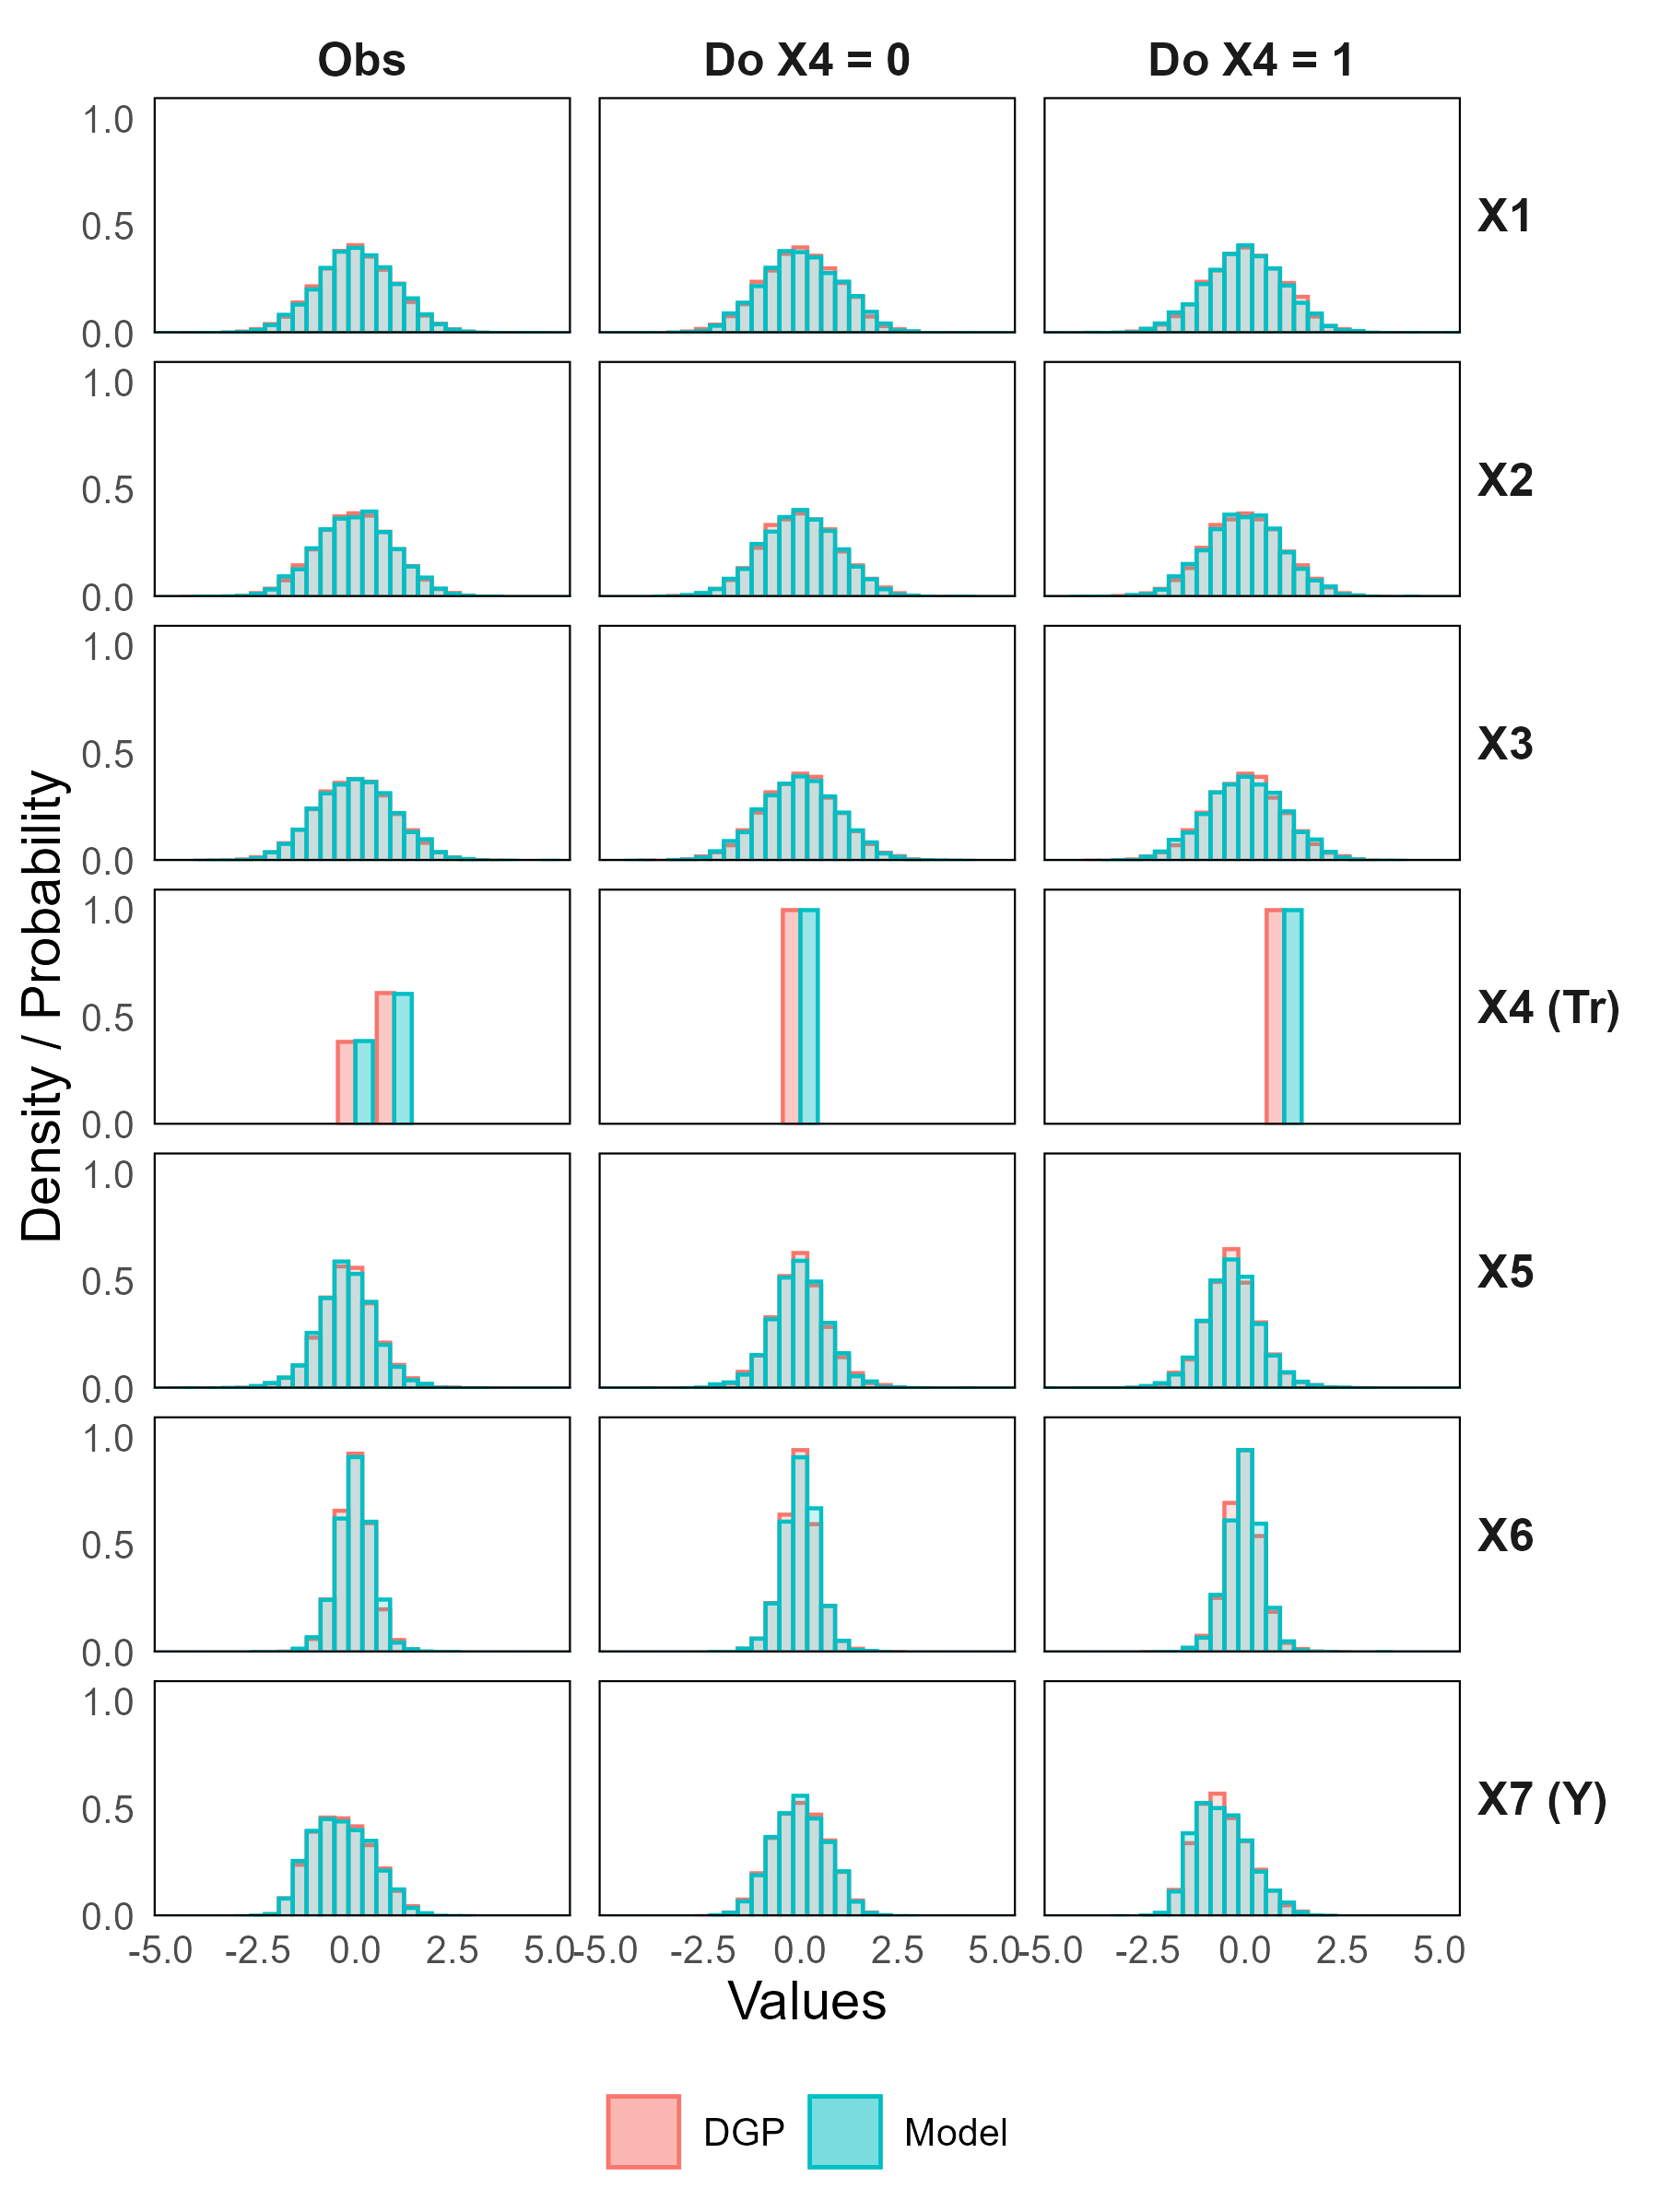
\includegraphics[width=0.45\textwidth]{img/results/observ_scenario1_sampling_distributions_vertical.png}
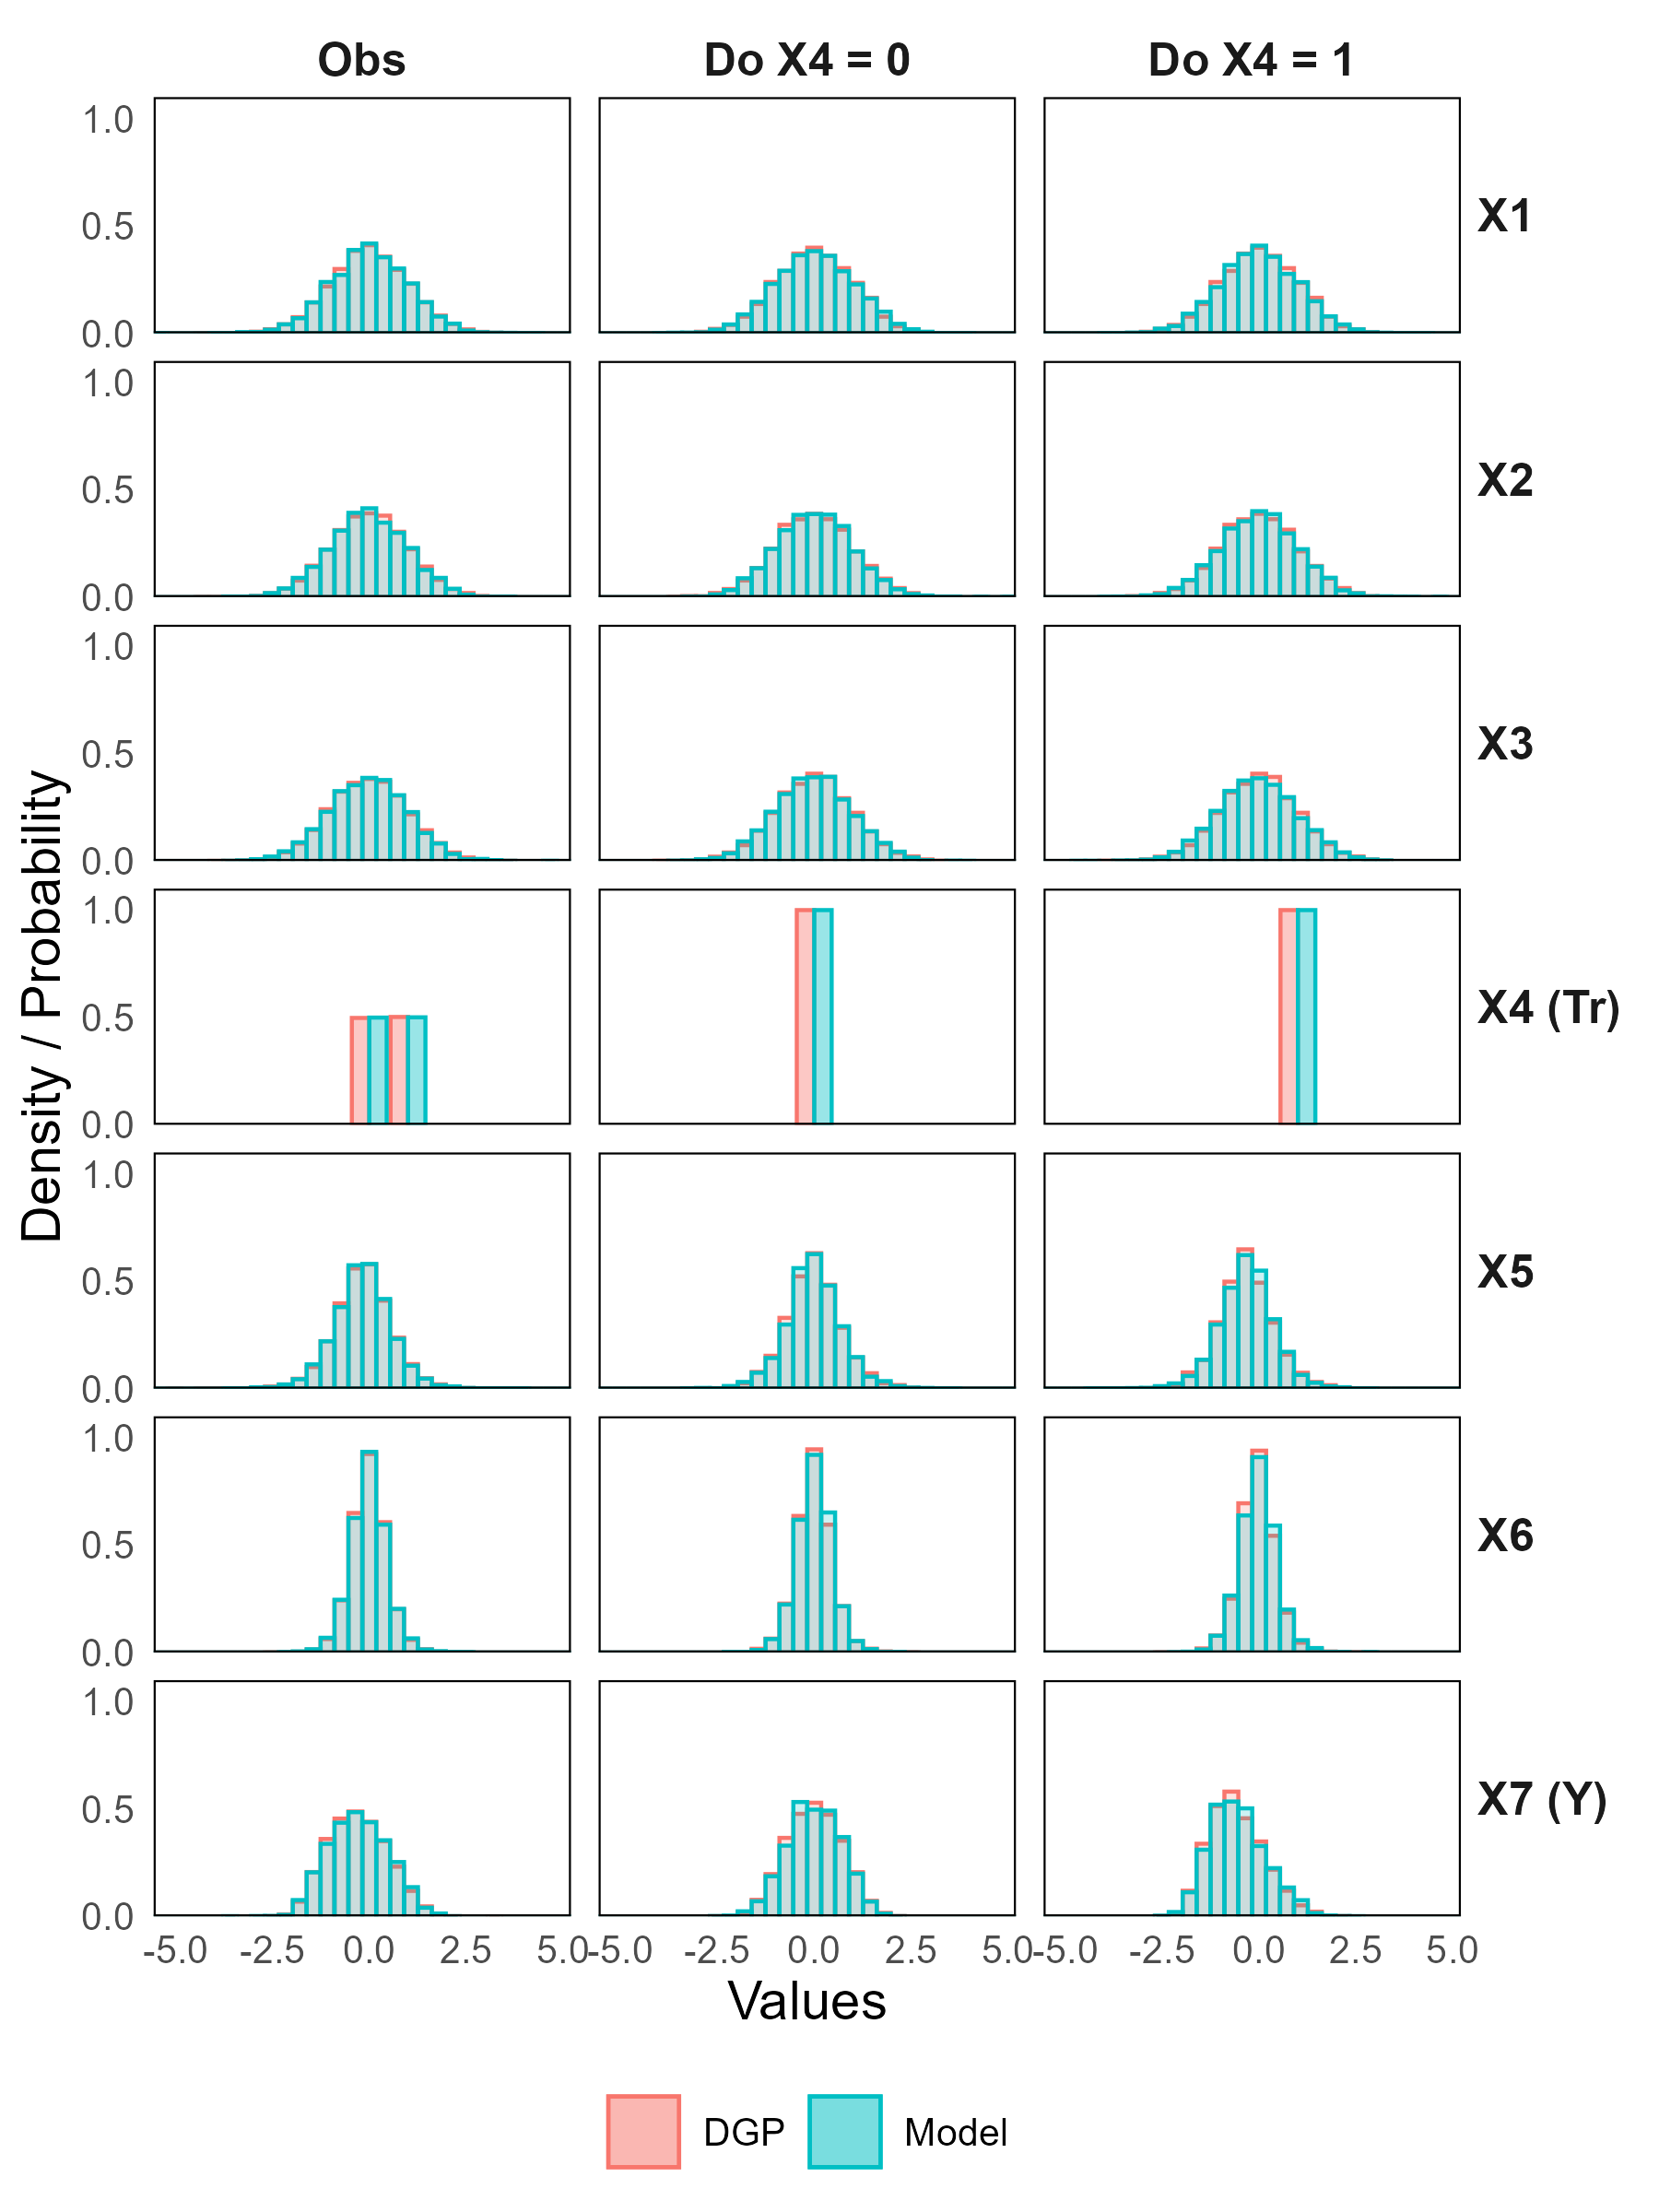
\includegraphics[width=0.45\textwidth]{img/results/rct_scenario1_sampling_distributions_vertical.png}
\caption{Marginal distributions of DGP variables and fitted TRAM-DAG samples for scenario (1) with direct and interaction effects. The distributions shown as observed (Obs), under control intervention (Do $X4=0$) and under treatment intervention (Do $X4=1$). Left: Observational; Right: RCT setting.}
\label{fig:scenario1_sampling_distributions_vertical}
\end{figure}

\begin{figure}[htbp]
\centering
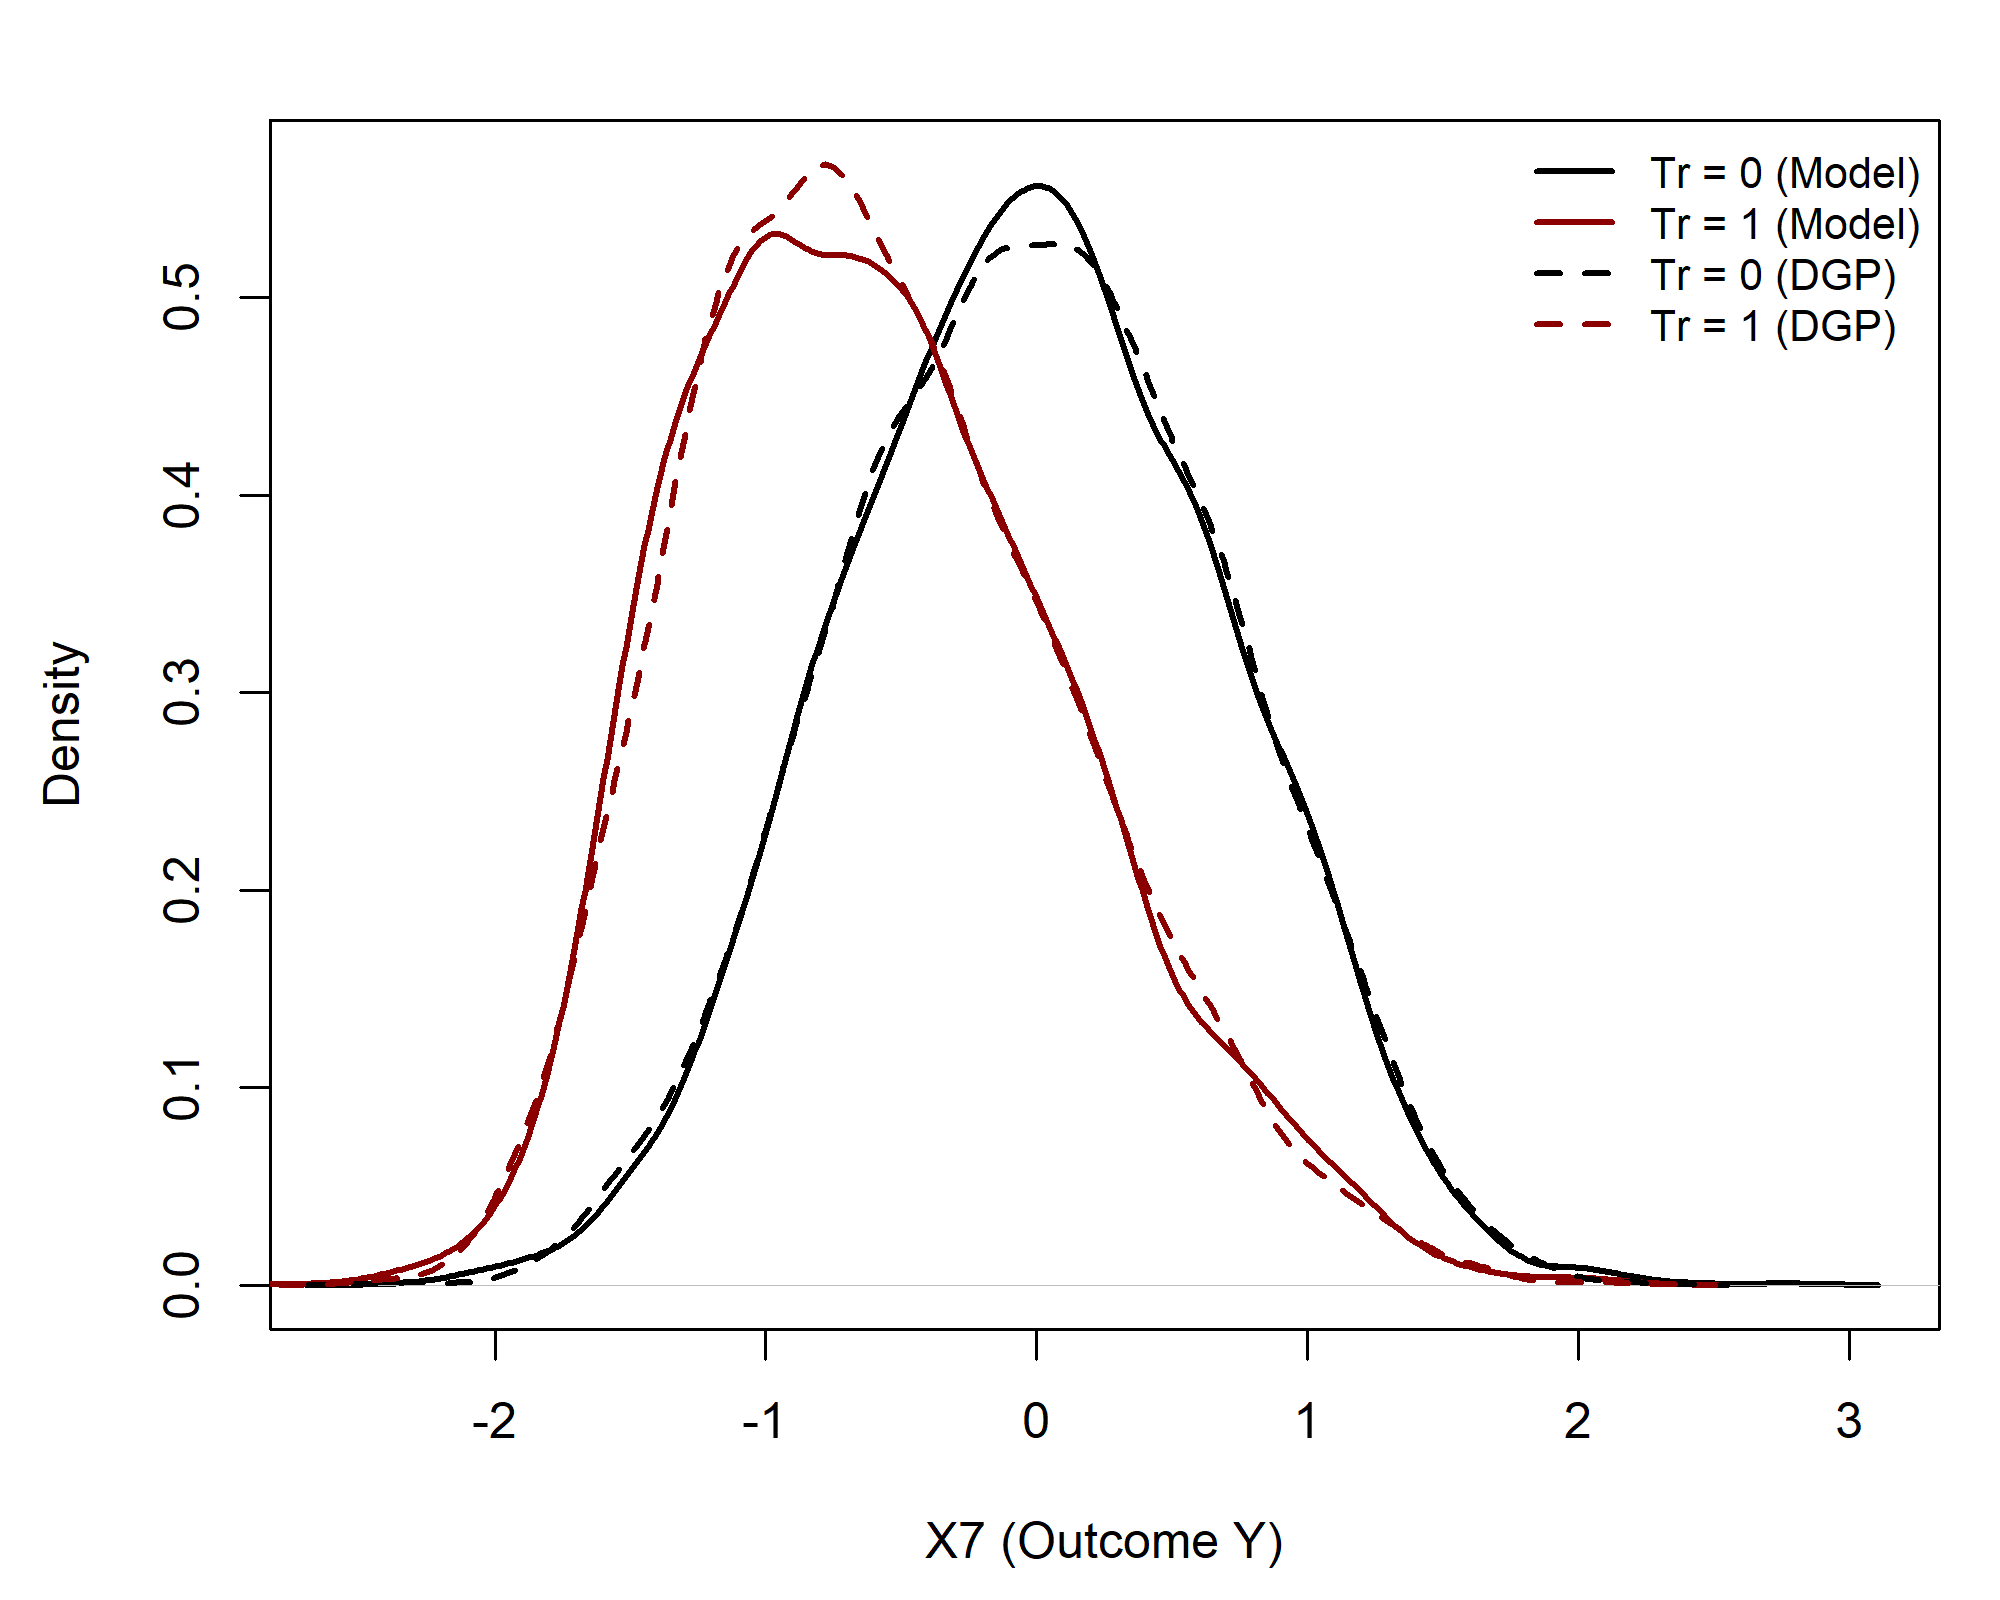
\includegraphics[width=0.45\textwidth]{img/results/observ_scenario1_X7_treatment_densities.png}
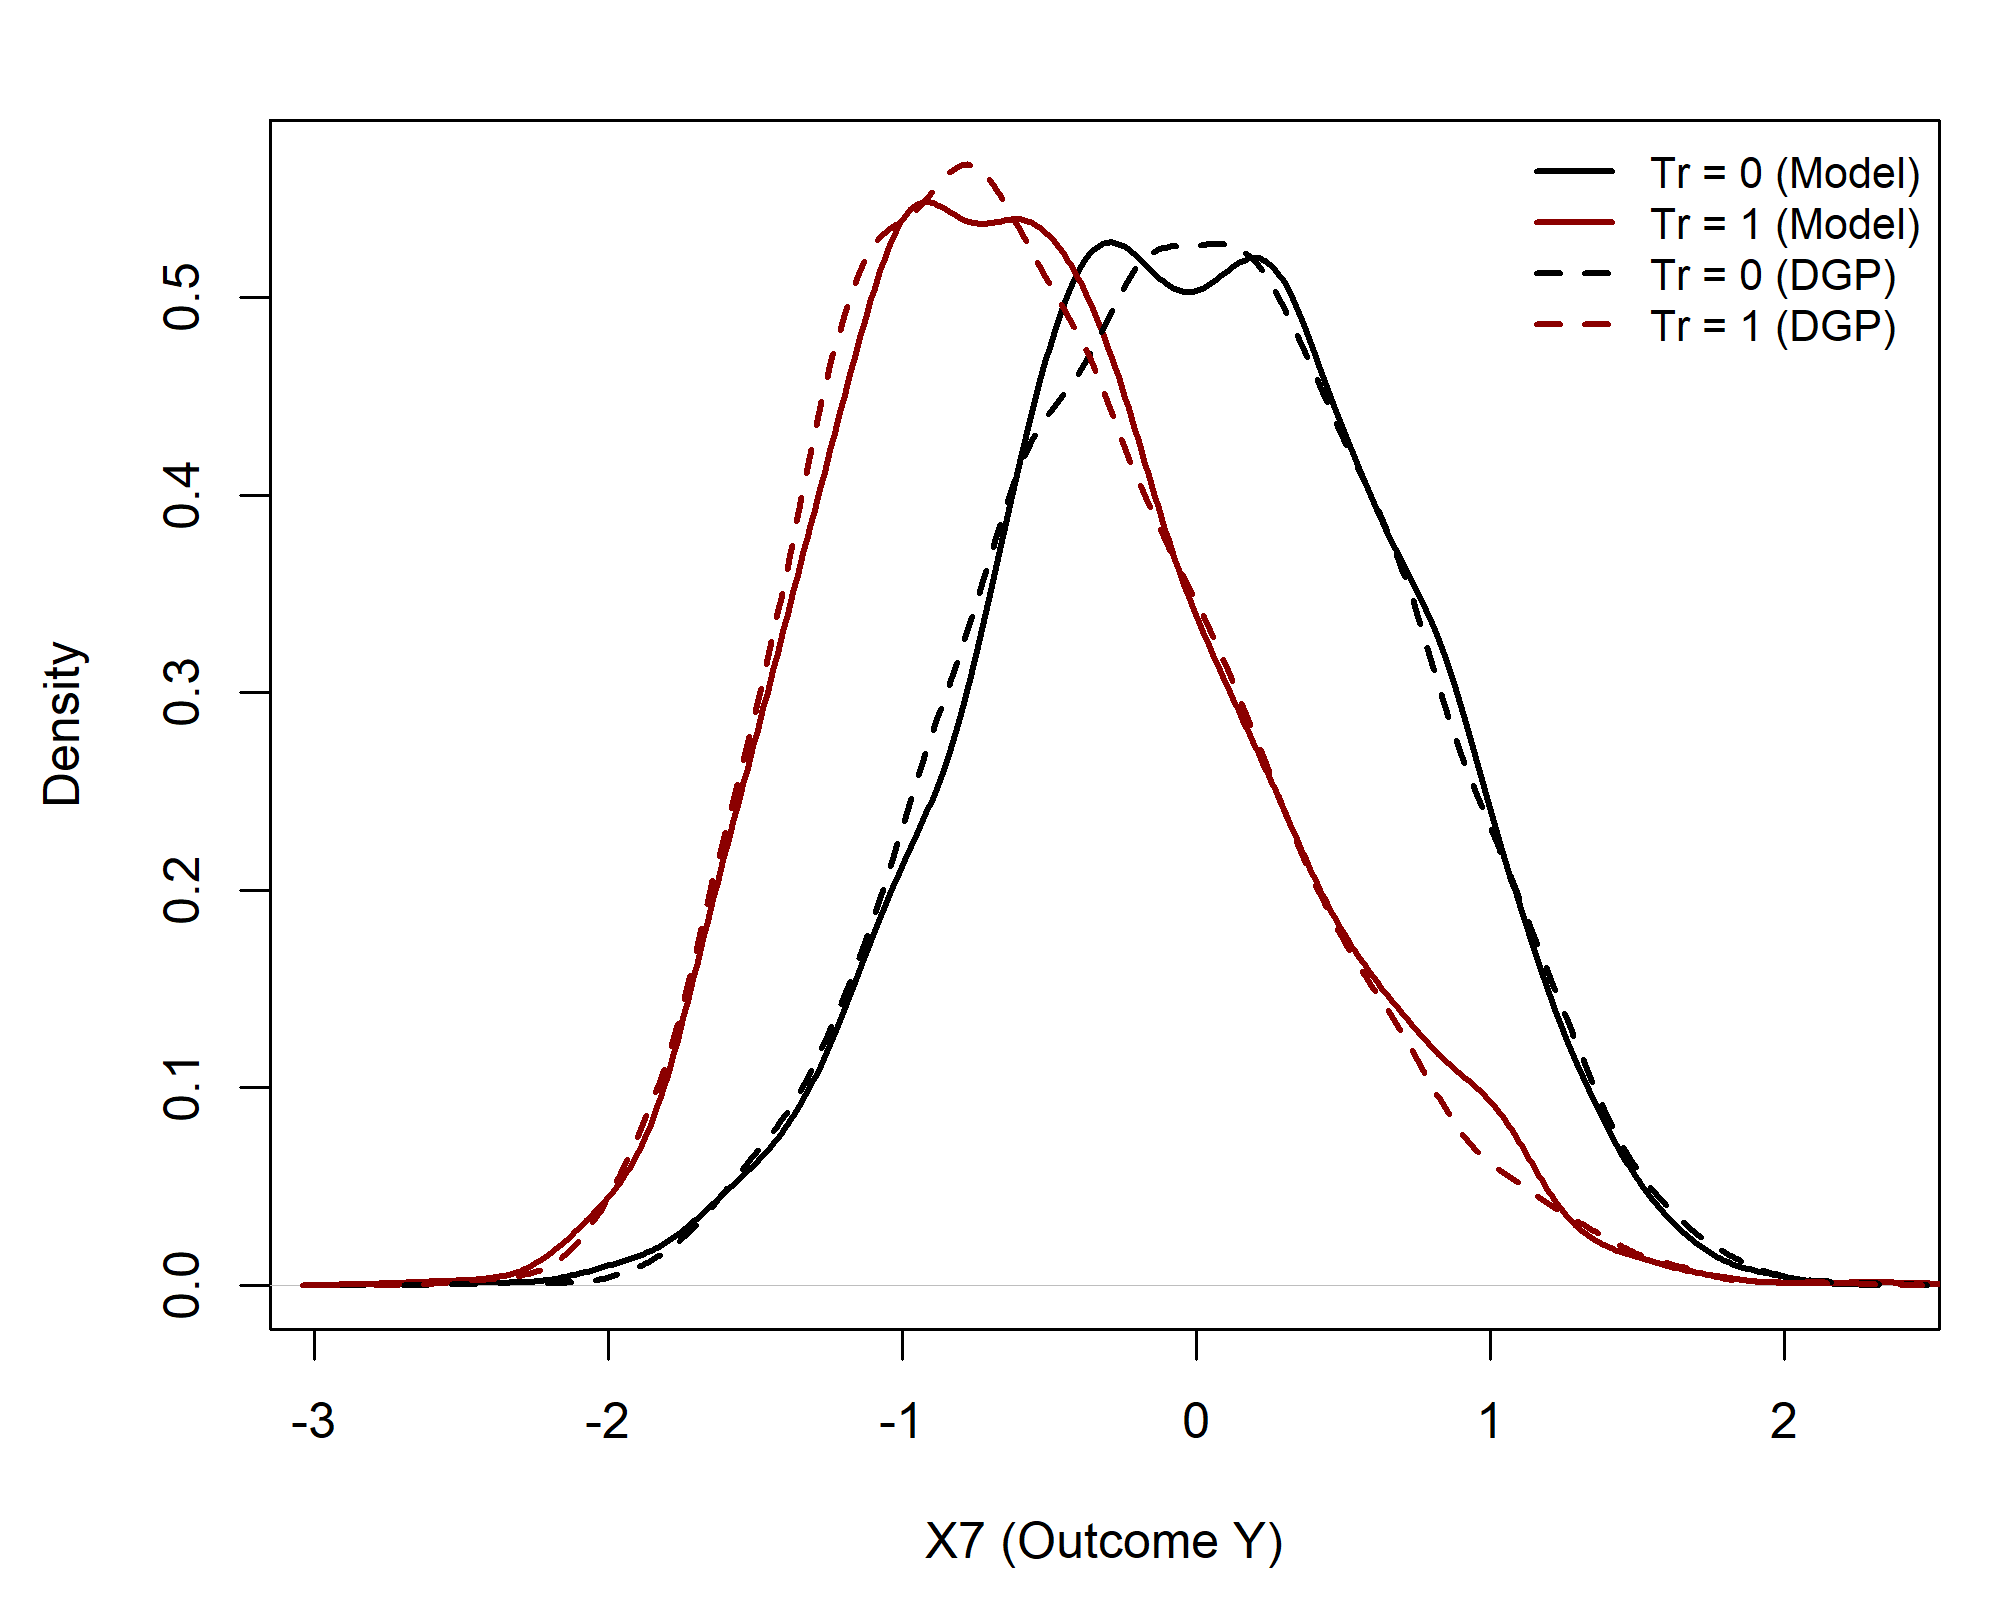
\includegraphics[width=0.45\textwidth]{img/results/rct_scenario1_X7_treatment_densities.png}
\caption{Distributions of the outcome variable (X7) under treatment and control interventions for scenario (1), including direct and interaction effects. This plot is a higher resolution view of the X7 panels (Do $X4=0$) and (Do $X4=1$) from Figure \ref{fig:scenario1_sampling_distributions_vertical}. Left: Observational; Right: RCT setting.}
\label{fig:scenario1_outcome_distributions}
\end{figure}




\begin{figure}[htbp]
\centering
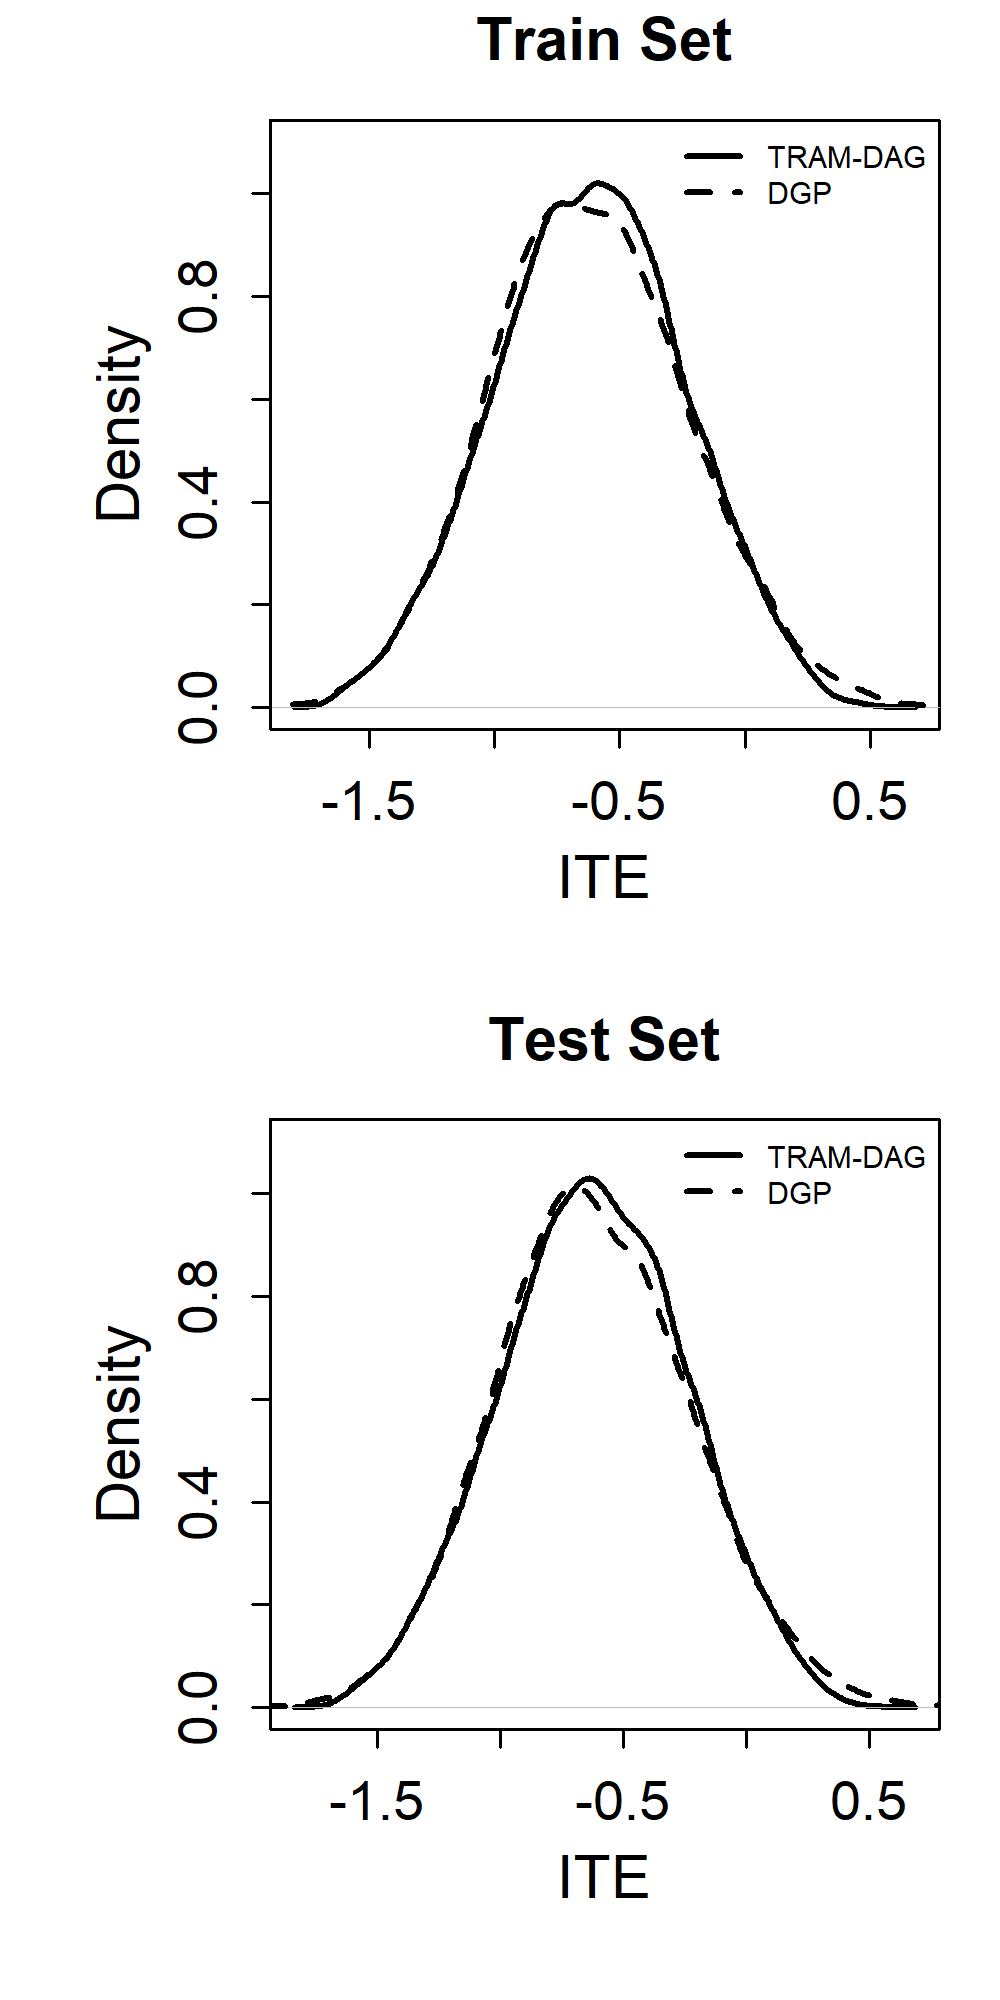
\includegraphics[width=0.45\textwidth]{img/results/observ_scenario1_ITE_densities_train_test.png}
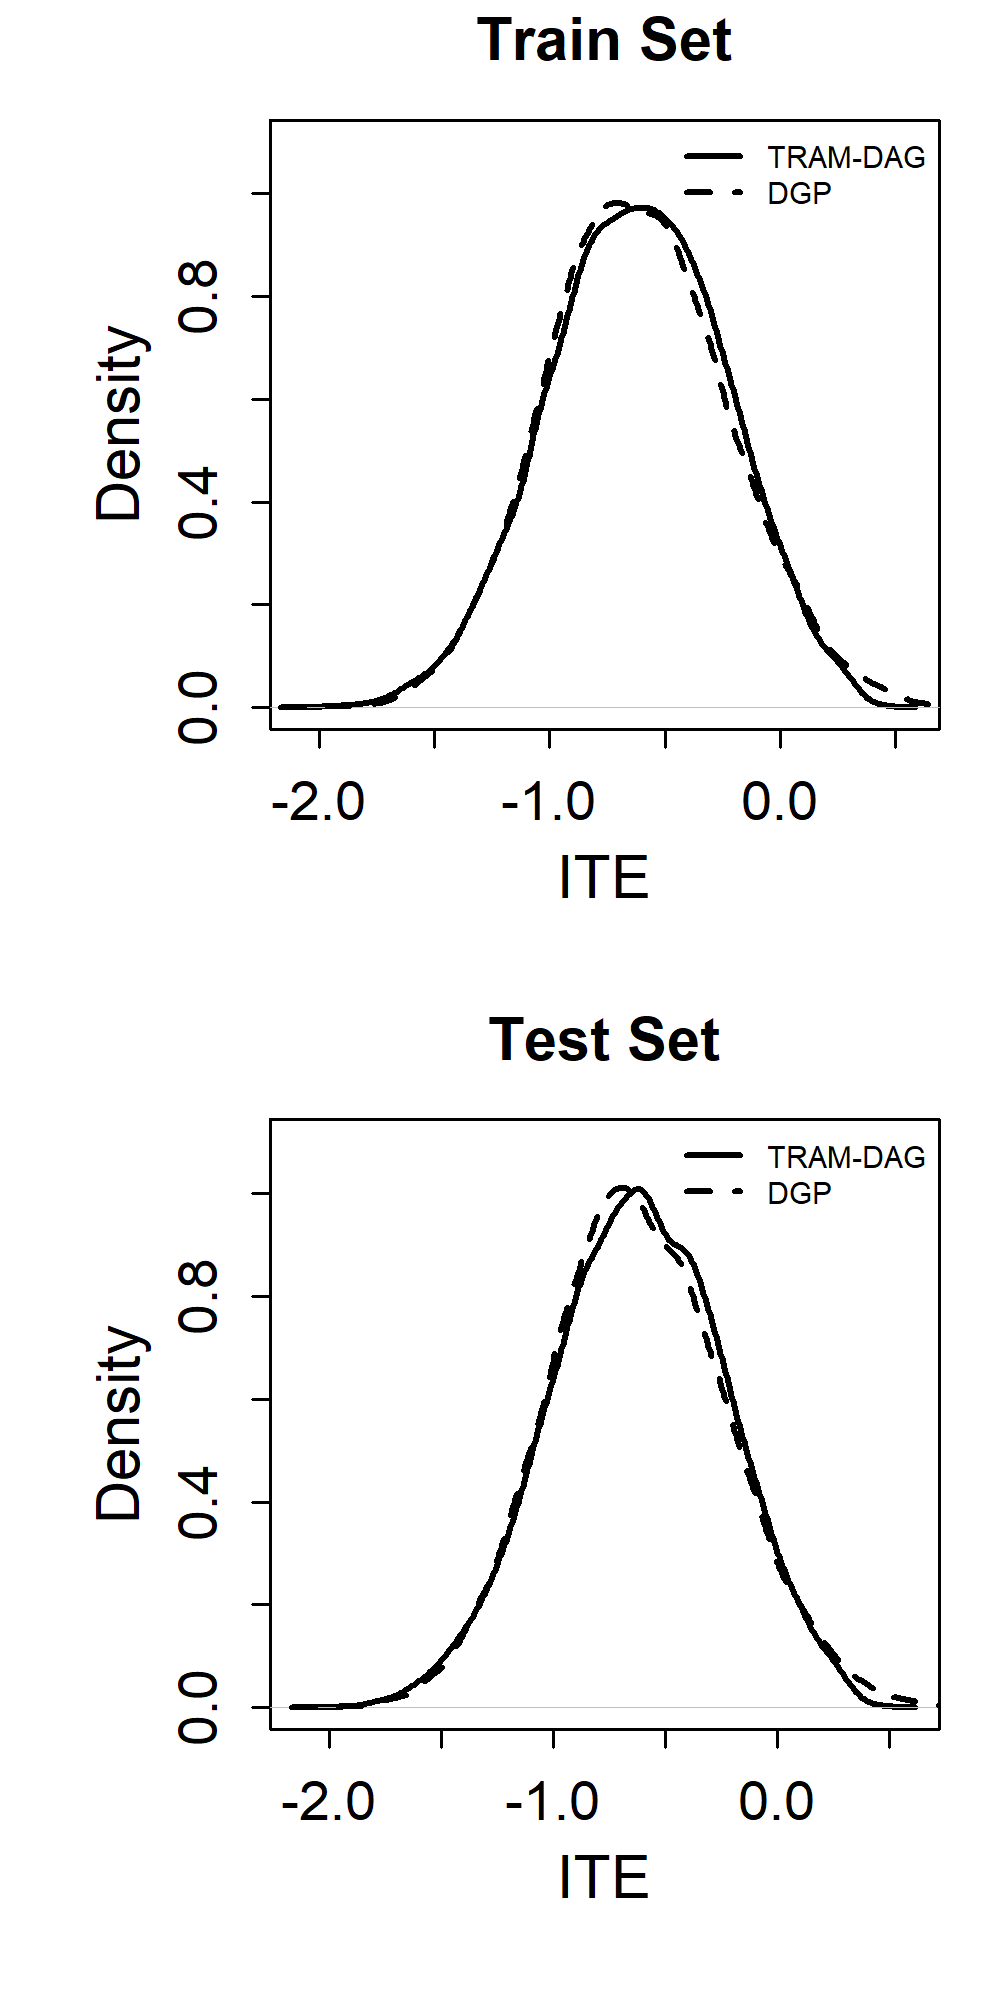
\includegraphics[width=0.45\textwidth]{img/results/rct_scenario1_ITE_densities_train_test.png}
\caption{Densities of estimated ITEs compared to the true ITEs in the training and test datasets for scenario (1), including direct and interaction effects. Left: Observational; right: RCT setting.}
\label{fig:scenario1_ite_densities_train_test}
\end{figure}






\begin{figure}[htbp]
\centering
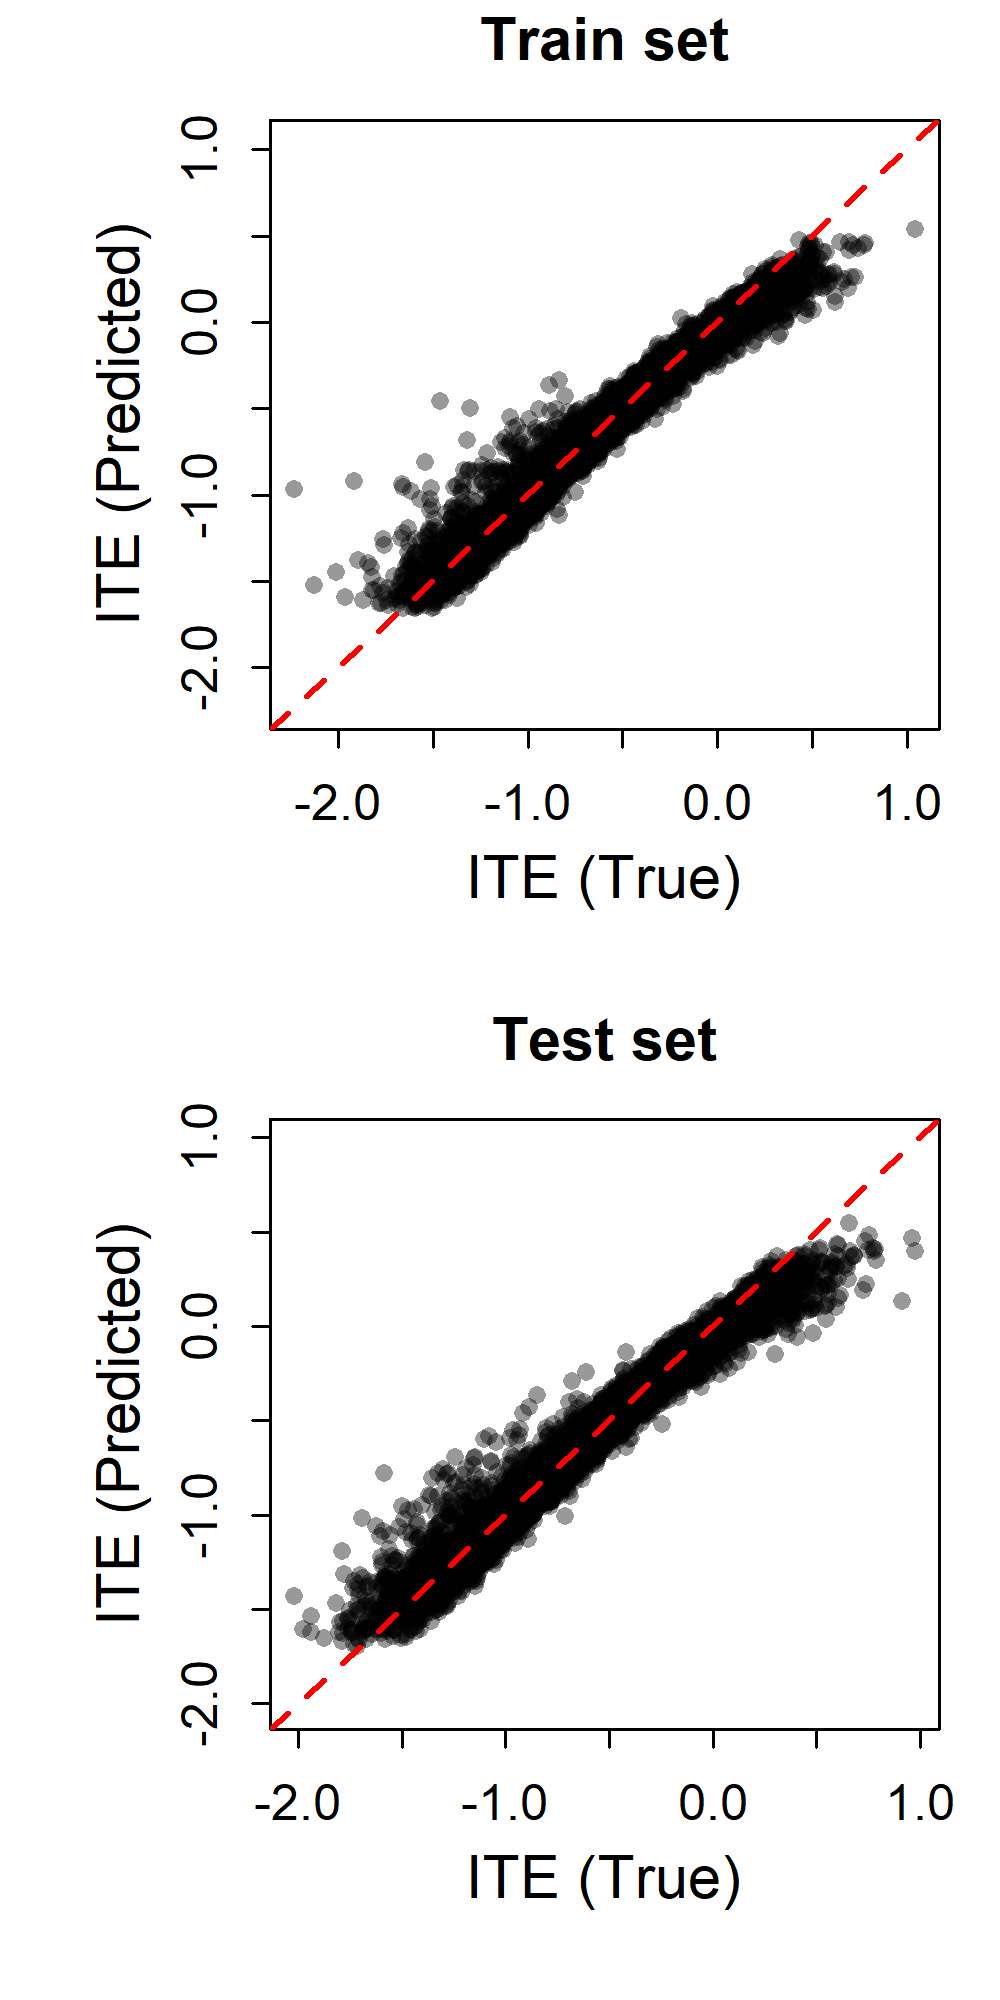
\includegraphics[width=0.45\textwidth]{img/results/observ_scenario1_ITE_scatter_train_test.png}
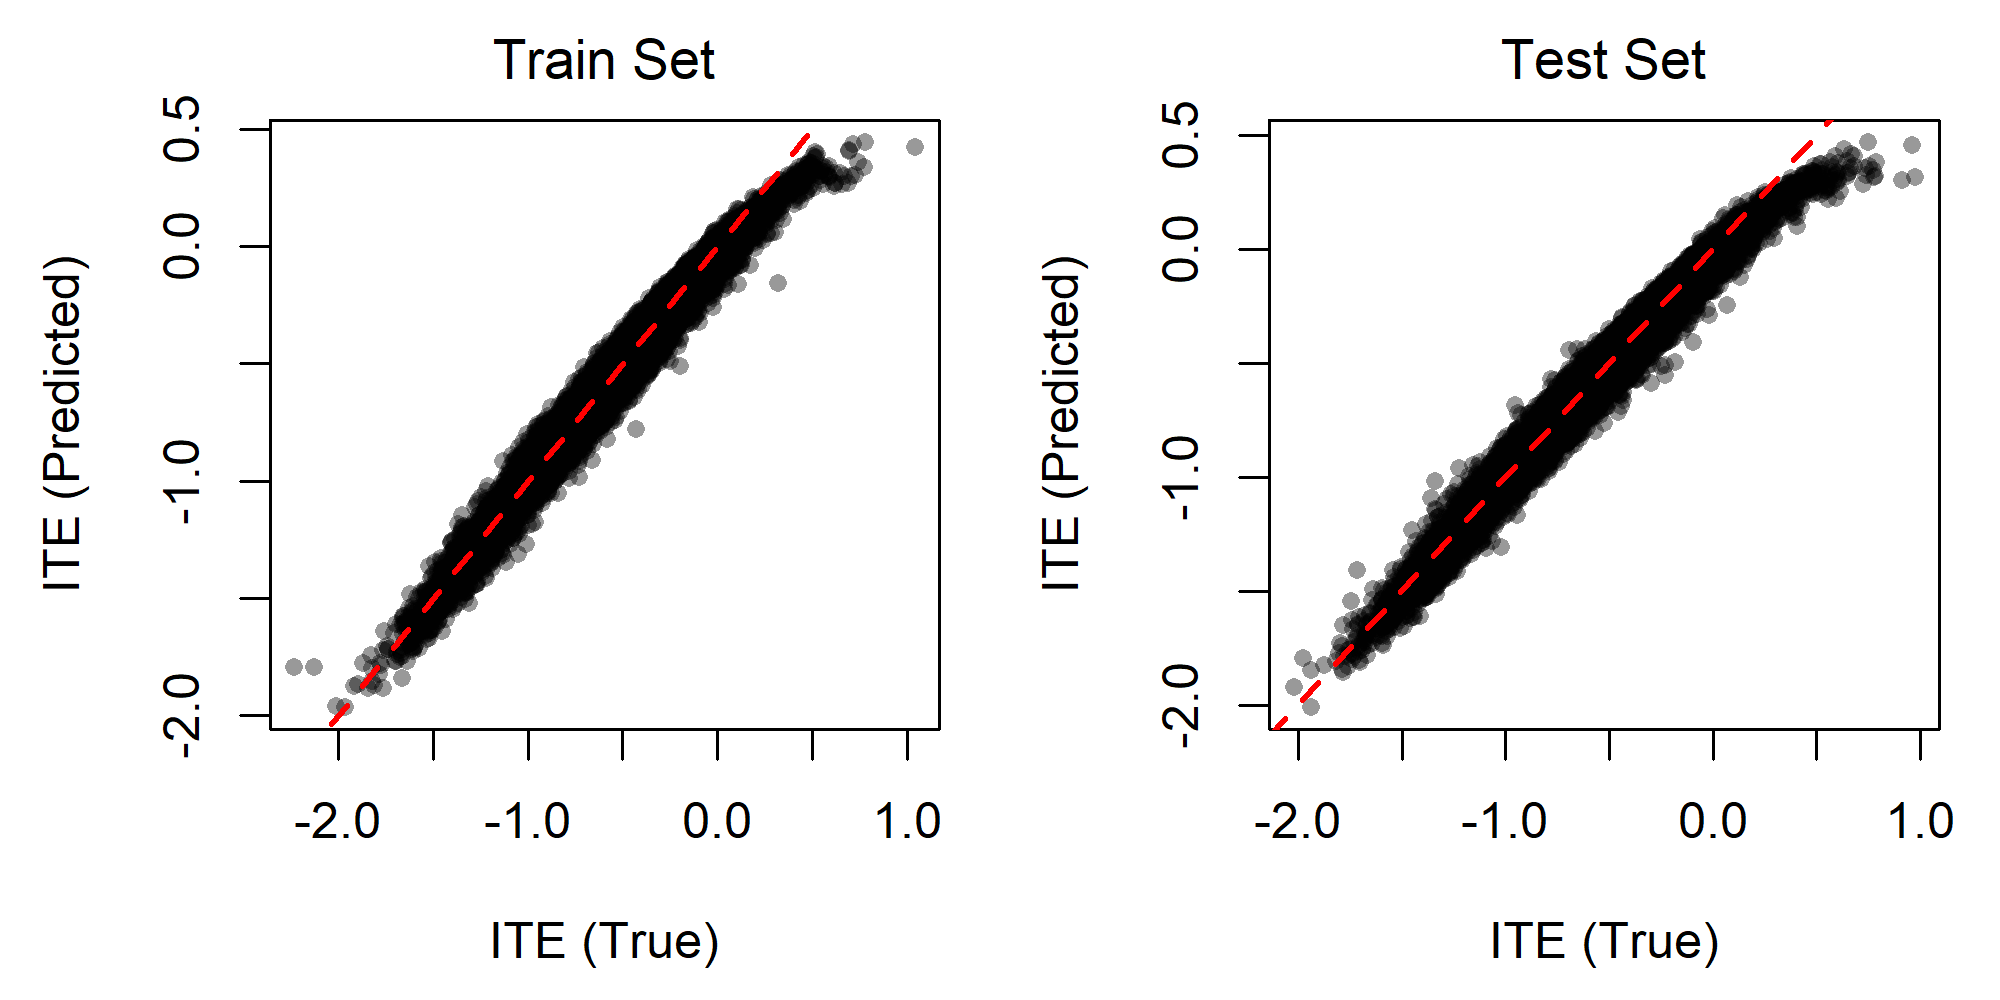
\includegraphics[width=0.45\textwidth]{img/results/rct_scenario1_ITE_scatter_train_test.png}
\caption{Scatterplots of estimated ITEs compared to the true ITEs in the training and test datasets for scenario (1), including direct and interaction effects. Left: Observational; right: RCT setting.}
\label{fig:scenario1_ite_scatter_train_test}
\end{figure}




\begin{figure}[htbp]
\centering
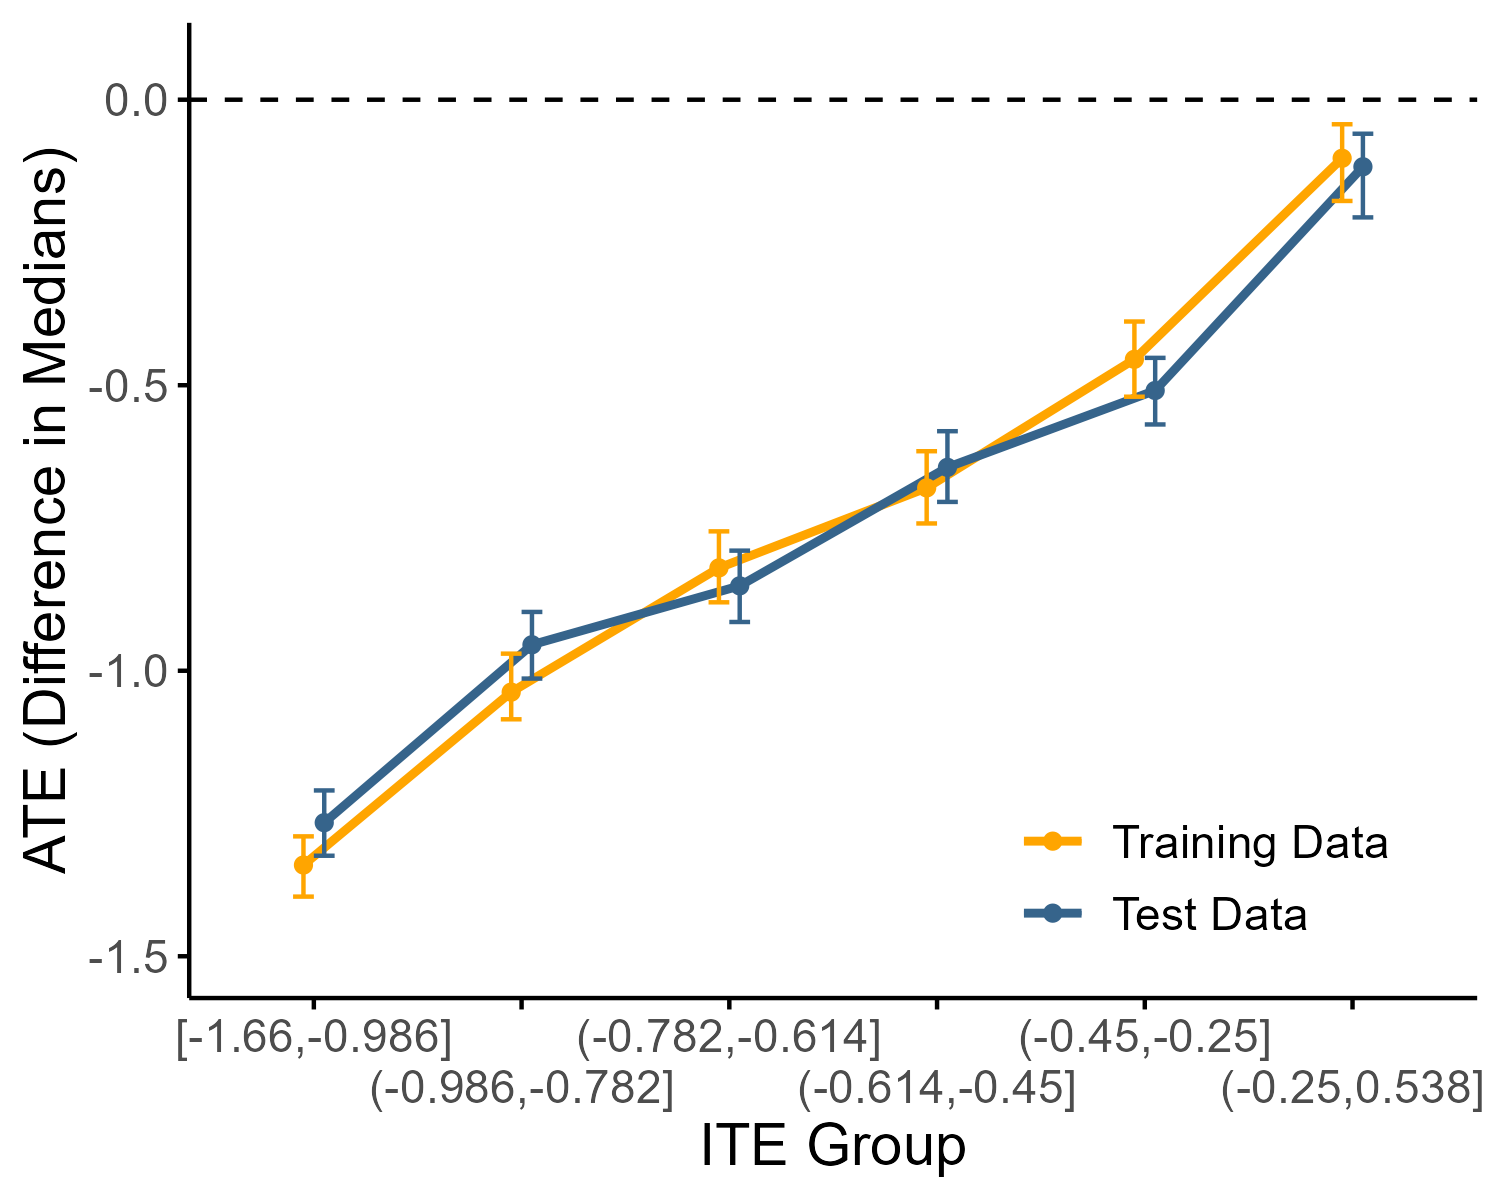
\includegraphics[width=0.45\textwidth]{img/results/observ_scenario1_ITE_cATE.png}
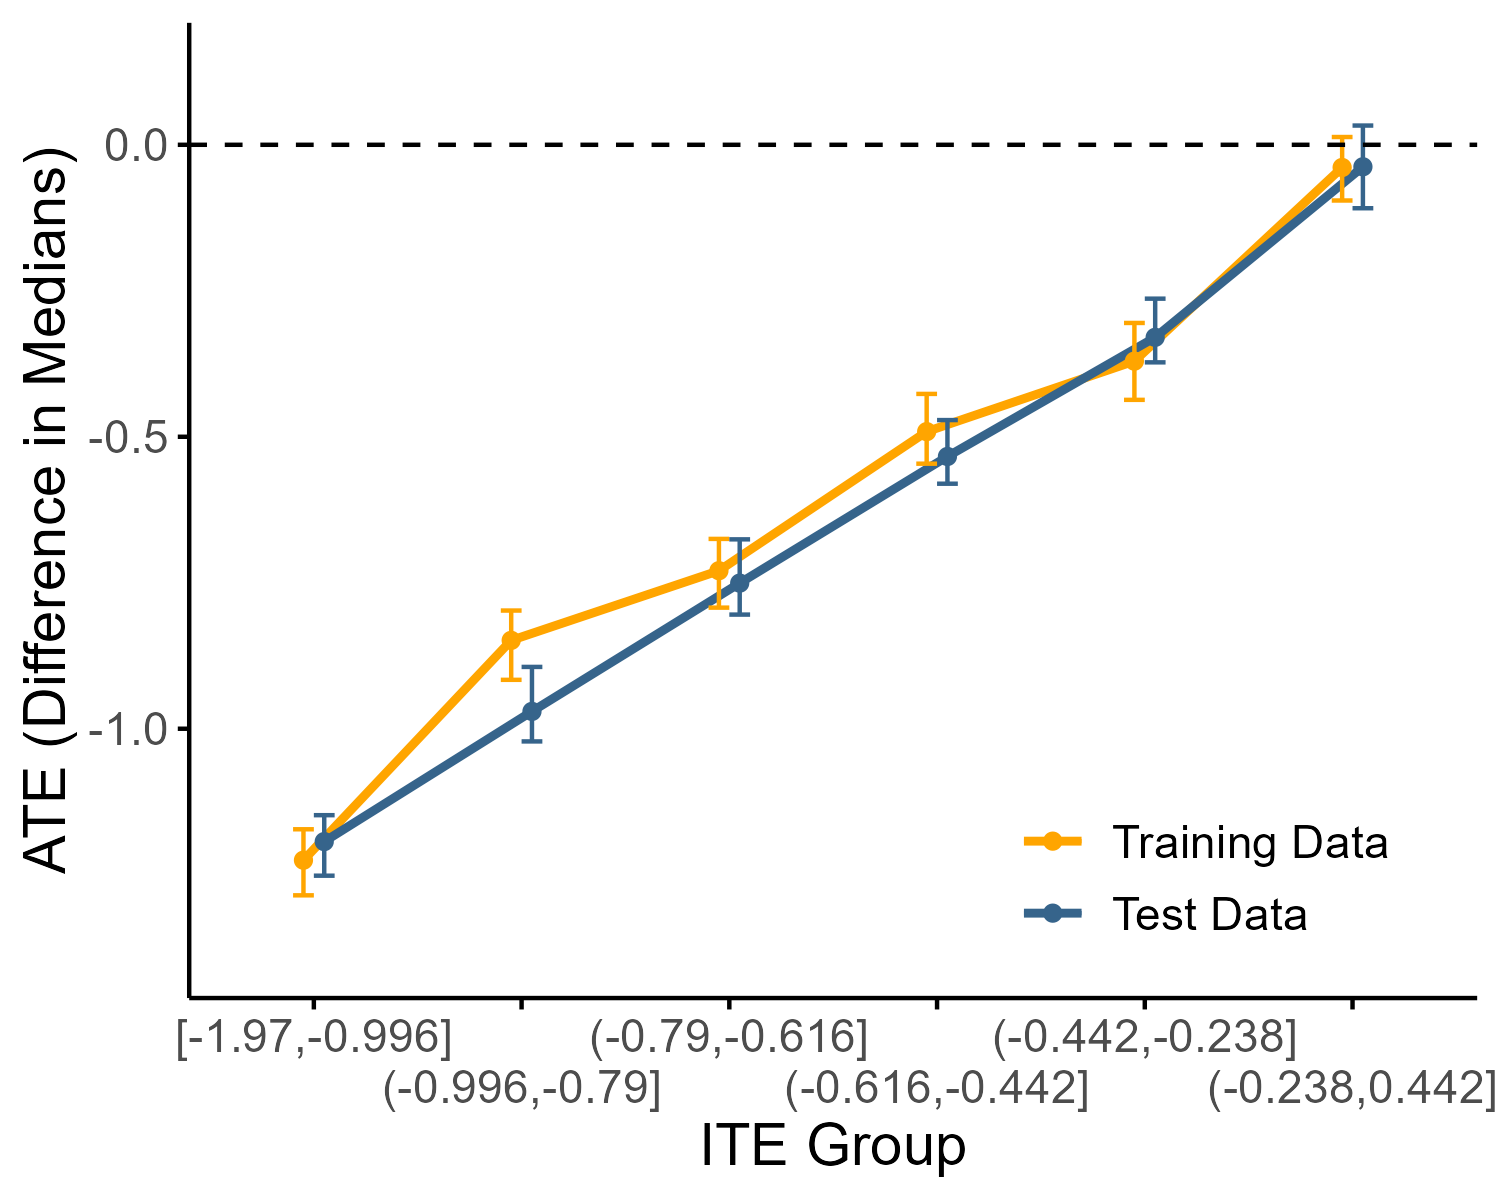
\includegraphics[width=0.45\textwidth]{img/results/rct_scenario1_ITE_cATE.png}
\caption{ITE-ATE plot for scenario (1), including direct and interaction effects. Individuals are grouped into bins according to the estimated ITE and in each bin the ATE is calculated as the difference in medians of the observed outcomes under the treatments. 95\% bootstrap confidence intervals indicate the uncertainty. Left: Observational; right: RCT setting.}
\label{fig:scenario1_ite_cATE}
\end{figure}



% start a new page
\clearpage


\subsection{Scenario (2): With direct but no interaction effects}

Scenario (2) included a direct effect of the treatment on the outcome and coefficients of the interaction effects are set to zero. This results in less heterogeneity of ITE compared to scenario (1) as shown in Figure \ref{fig:scenario2_ite_distribution_dgp}. The observational and interventional densities sampled by the fitted TRAM-DAG are aligned with the true densities according to the DGP as illustrated in Figures \ref{fig:scenario2_sampling_distributions_vertical} and \ref{fig:scenario2_outcome_distributions}. A notable discrepancy in variance exists between the estimated and true ITEs, as illustrated in Figures \ref{fig:scenario2_ite_densities_train_test} and \ref{fig:scenario2_ite_scatter_train_test}. The ITE-ATE plot in Figure \ref{fig:scenario2_ite_cATE} shows a less informative view compared to scenario (1). Table \ref{tab:scenario2_ate_comparison} presents the ATE measures for scenario (2). In the test set of the RCT setting, the ATE in terms of the difference in medians of the observed outcomes was $-0.639$. In contrast, the ATE based on the estimated ITEs in the same dataset was $-0.586$.


\begin{table}[htbp]
\centering
\small
\caption{Scenario (2), including a direct treatment but no interaction effects: Comparison of ATE measures across train and test sets for the observational and RCT setting.}
\label{tab:scenario2_ate_comparison}
\begin{tabular}{l c c c c}
\toprule
\textbf{Measure} & \multicolumn{2}{c}{\textbf{Observational}} & \multicolumn{2}{c}{\textbf{RCT}} \\
\cmidrule(lr){2-3} \cmidrule(lr){4-5}
 & \textbf{Train} & \textbf{Test} & \textbf{Train} & \textbf{Test} \\
\midrule
ATE as $\text{mean}(\text{Y}_\text{observed}^{(1)}) - \text{mean}(\text{Y}_\text{observed}^{(0)})$ & NA & NA & -0.569 & -0.572 \\
ATE as $\text{median}(\text{Y}_\text{observed}^{(1)}) - \text{median}(\text{Y}_\text{observed}^{(0)})$  & NA & NA & -0.629 & -0.639 \\
ATE as mean(ITE$_\text{true}$)  & -0.633 & -0.633 & -0.633 & -0.633 \\
ATE as mean(ITE$_\text{estimated}$) & -0.645 & -0.644 & -0.587 & -0.586 \\
\bottomrule
\end{tabular}
\end{table}



\begin{figure}[htbp]
\centering
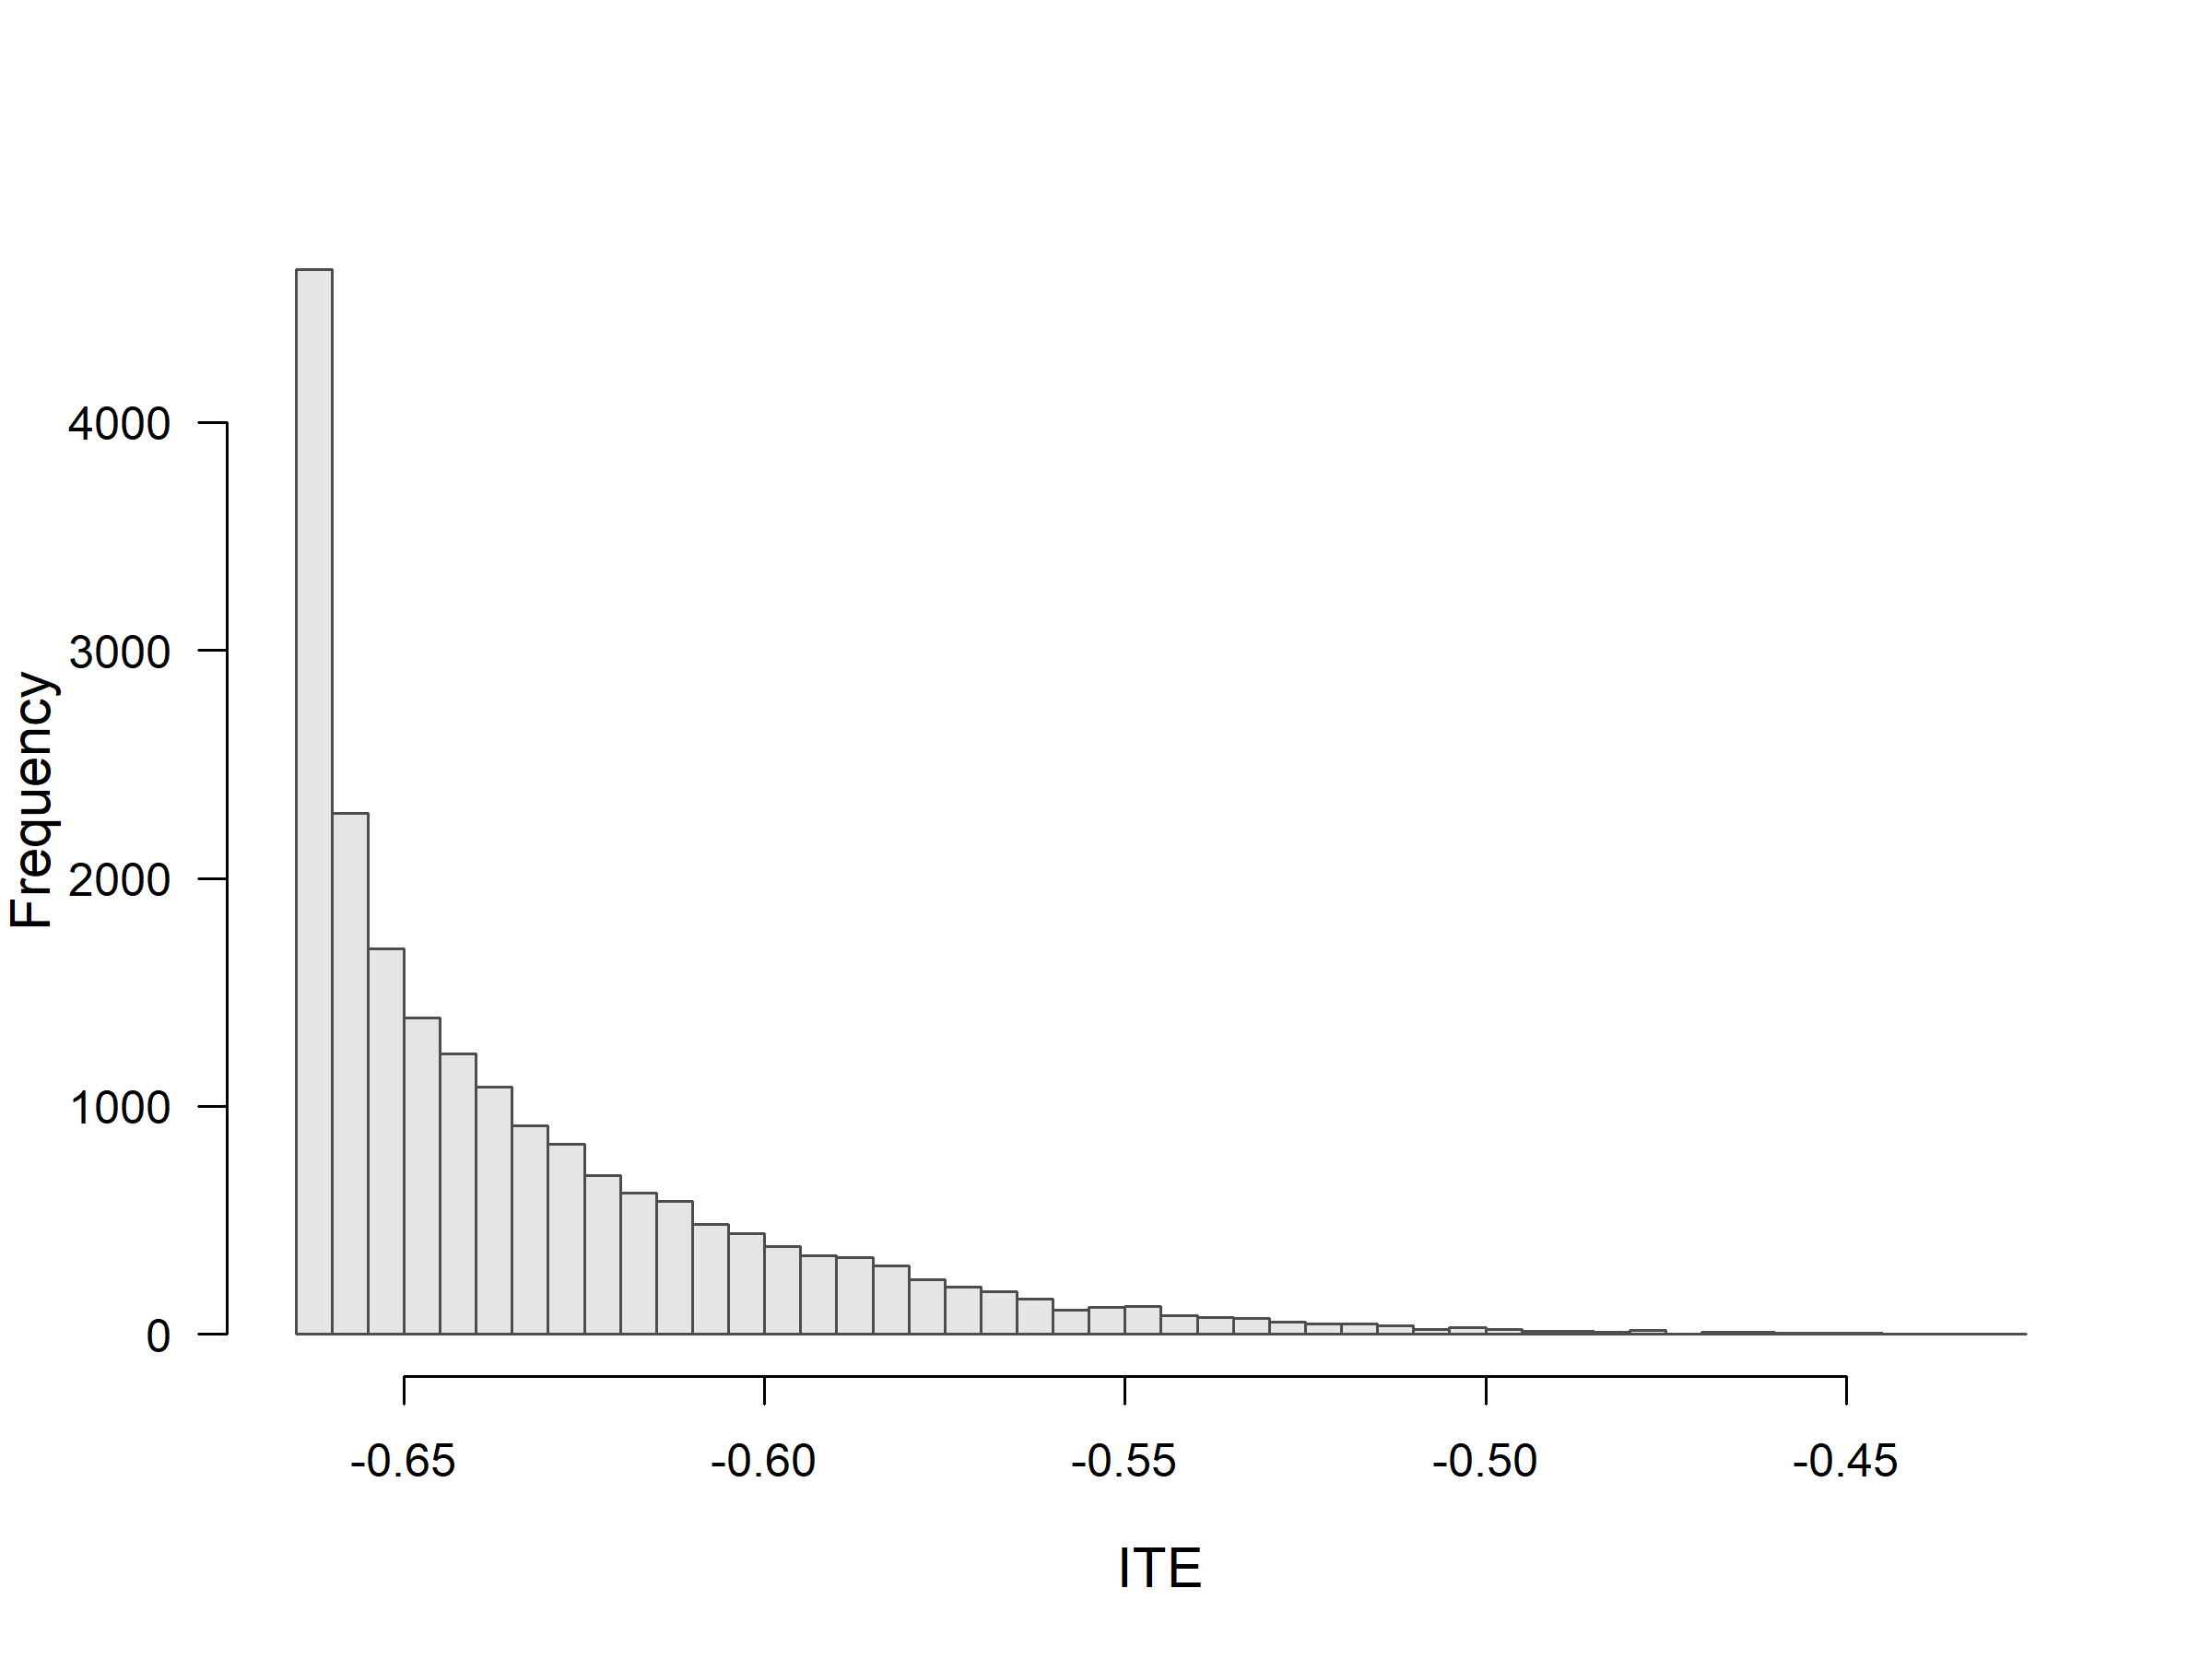
\includegraphics[width=0.45\textwidth]{img/results/observ_scenario2_ite_distribution_dgp.png}
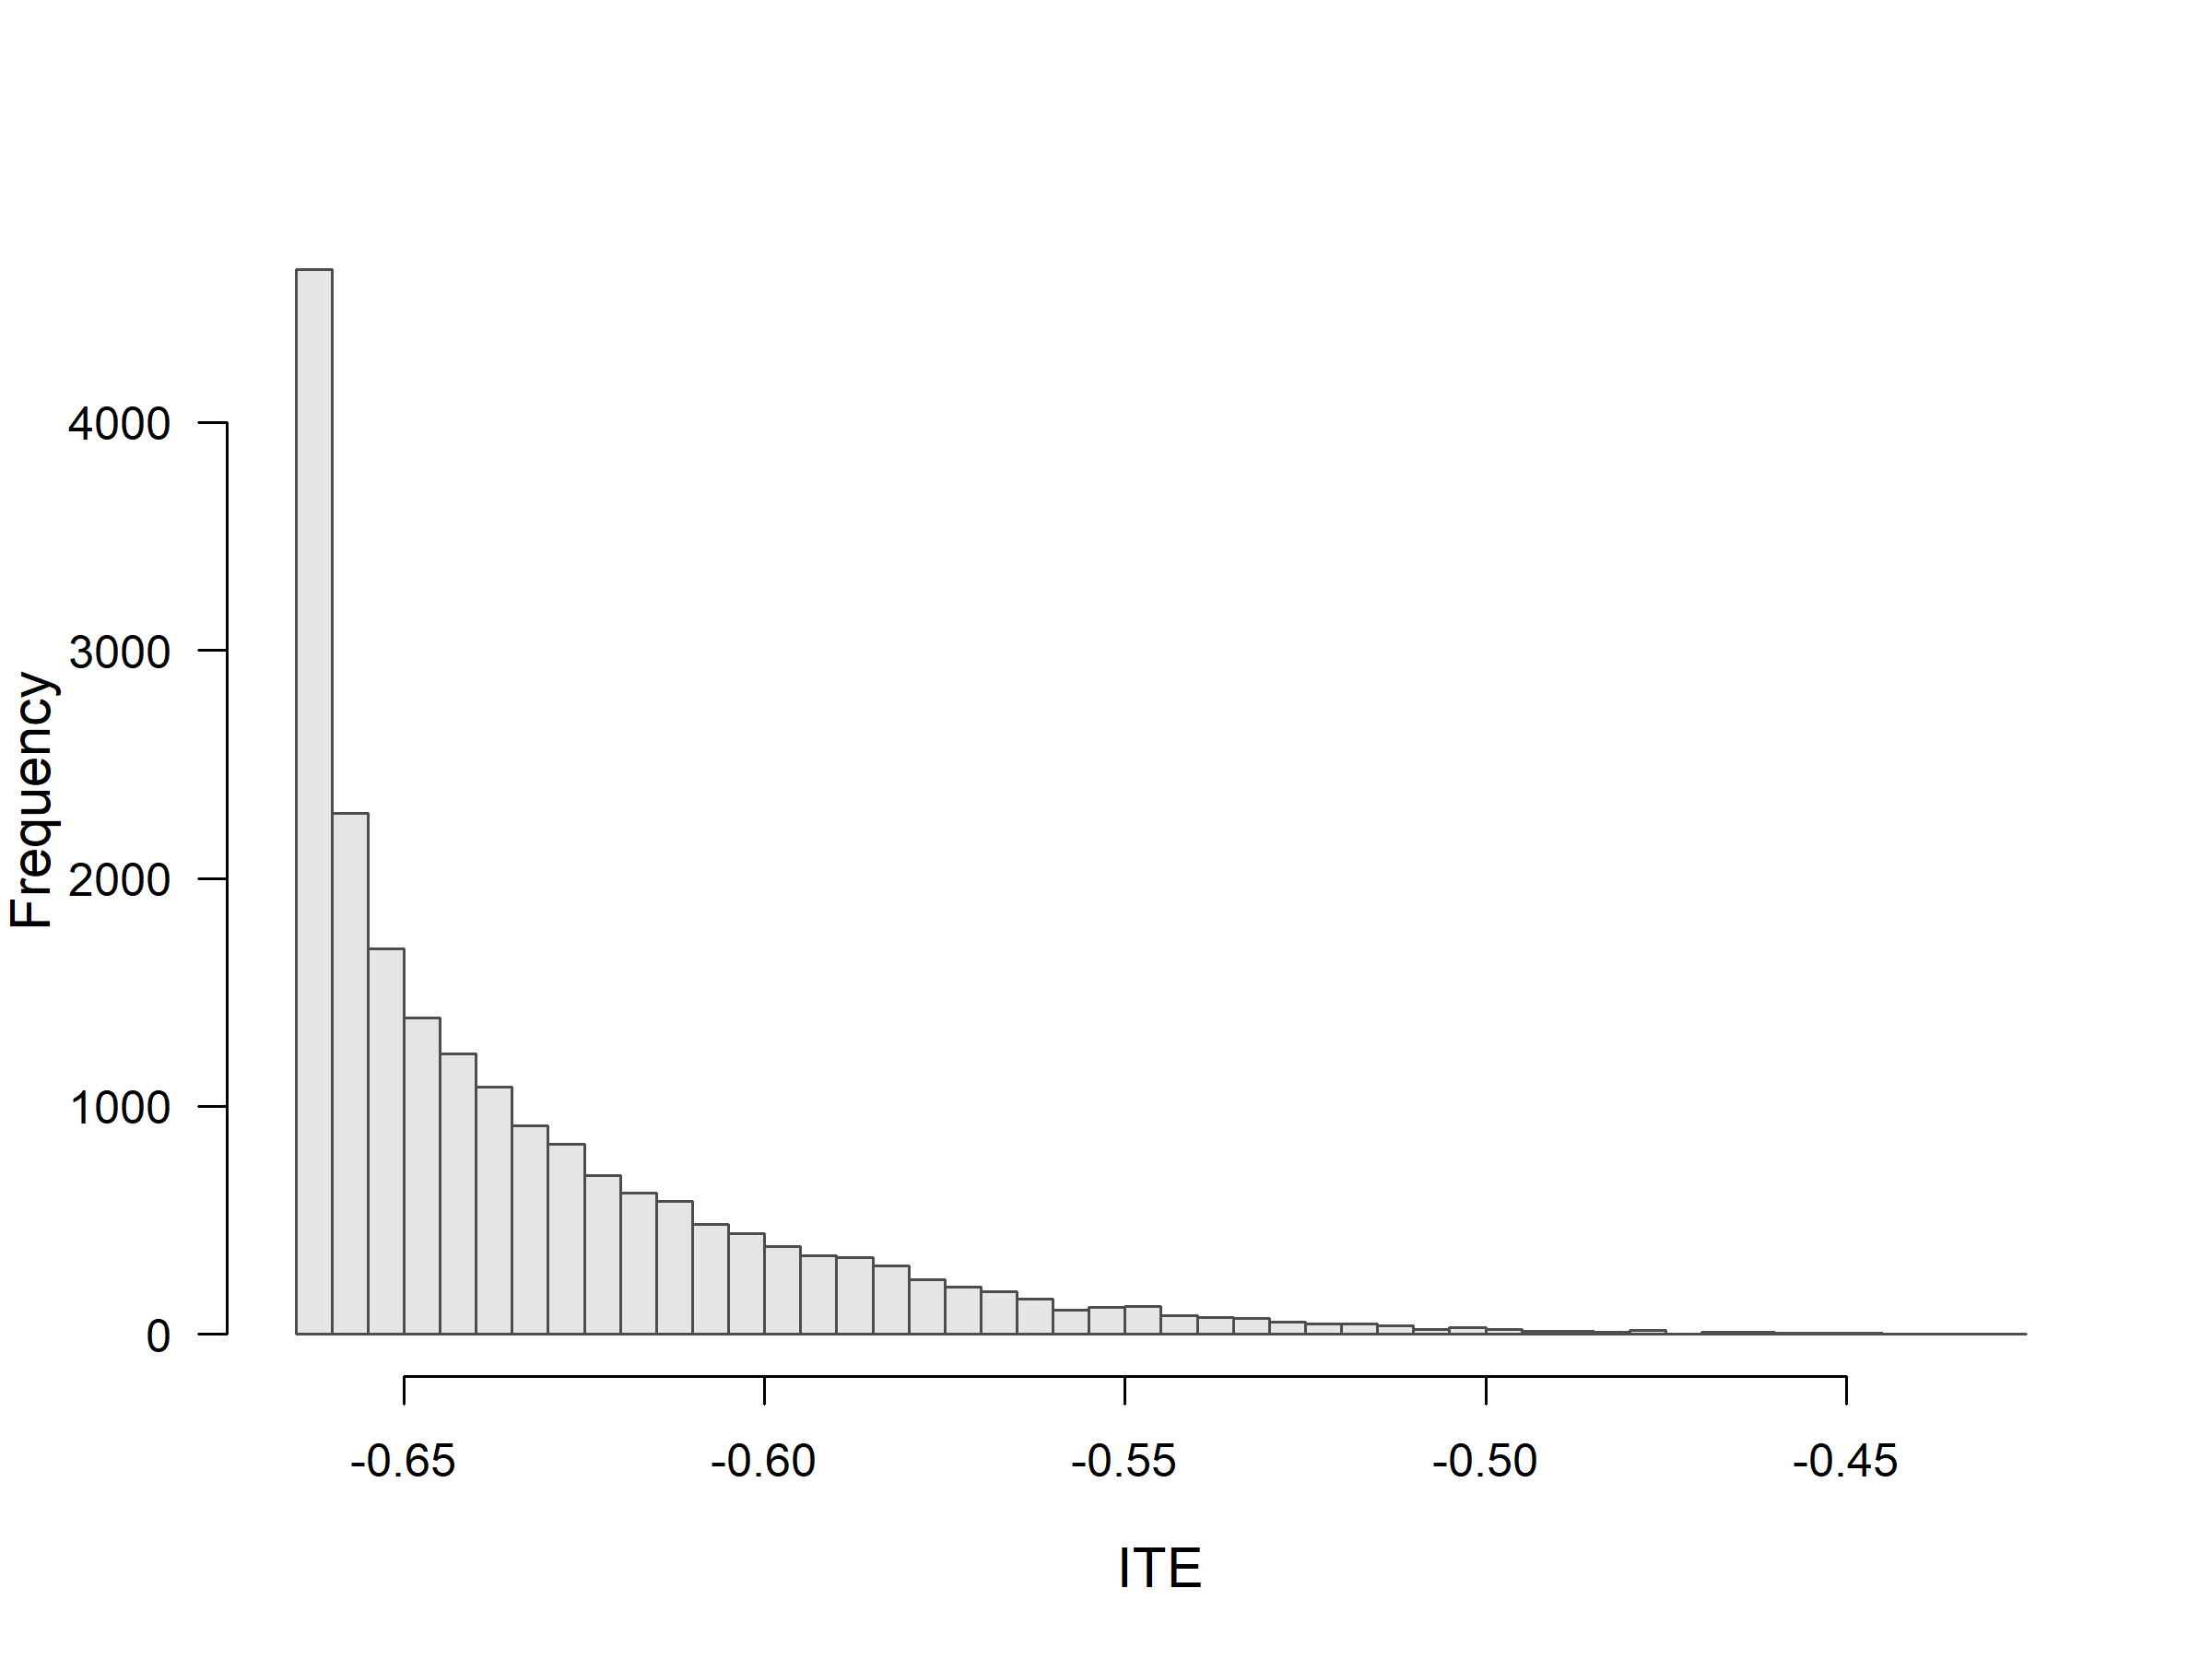
\includegraphics[width=0.45\textwidth]{img/results/rct_scenario2_ite_distribution_dgp.png}
\caption{True ITE distribution resulting from the DGP for scenario (2), including a direct treatment but no interaction effects. The true ITEs are identical in the observational and in the RCT setting, since they depend on the potential outcomes under both treatment allocations. Left: Observational; Right: RCT setting.}
\label{fig:scenario2_ite_distribution_dgp}
\end{figure}



\begin{figure}[htbp]
\centering
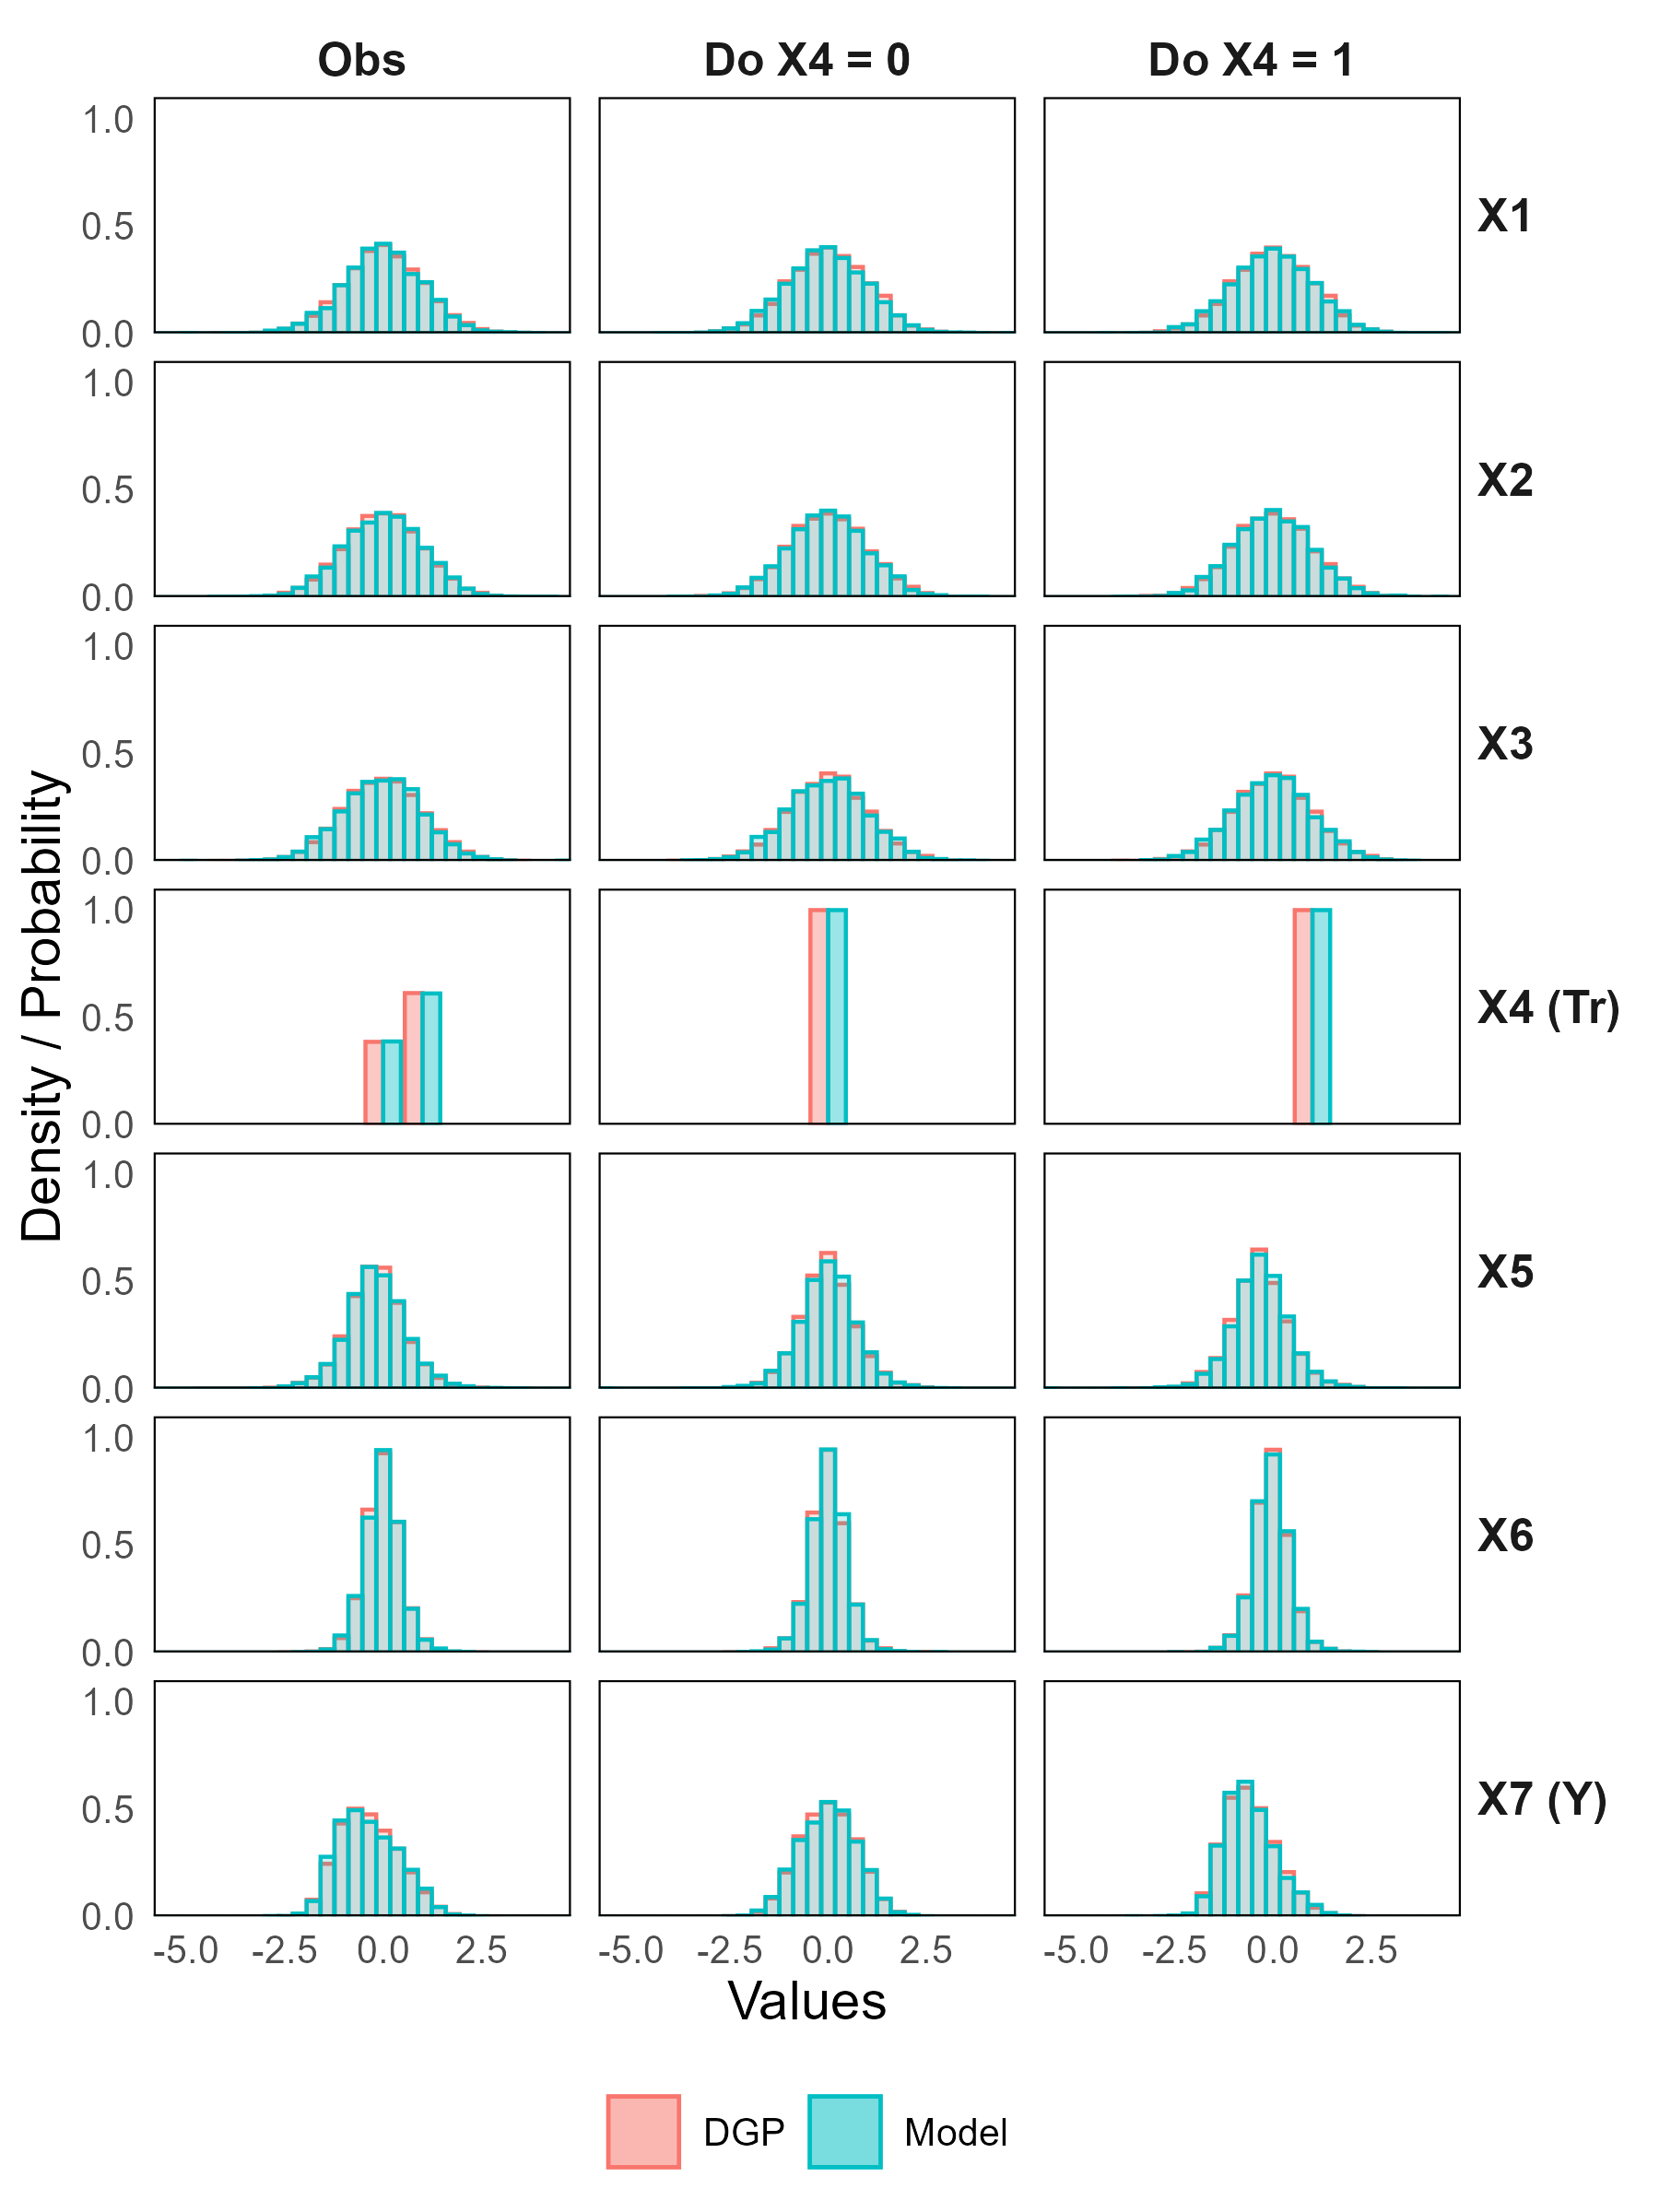
\includegraphics[width=0.45\textwidth]{img/results/observ_scenario2_sampling_distributions_vertical.png}
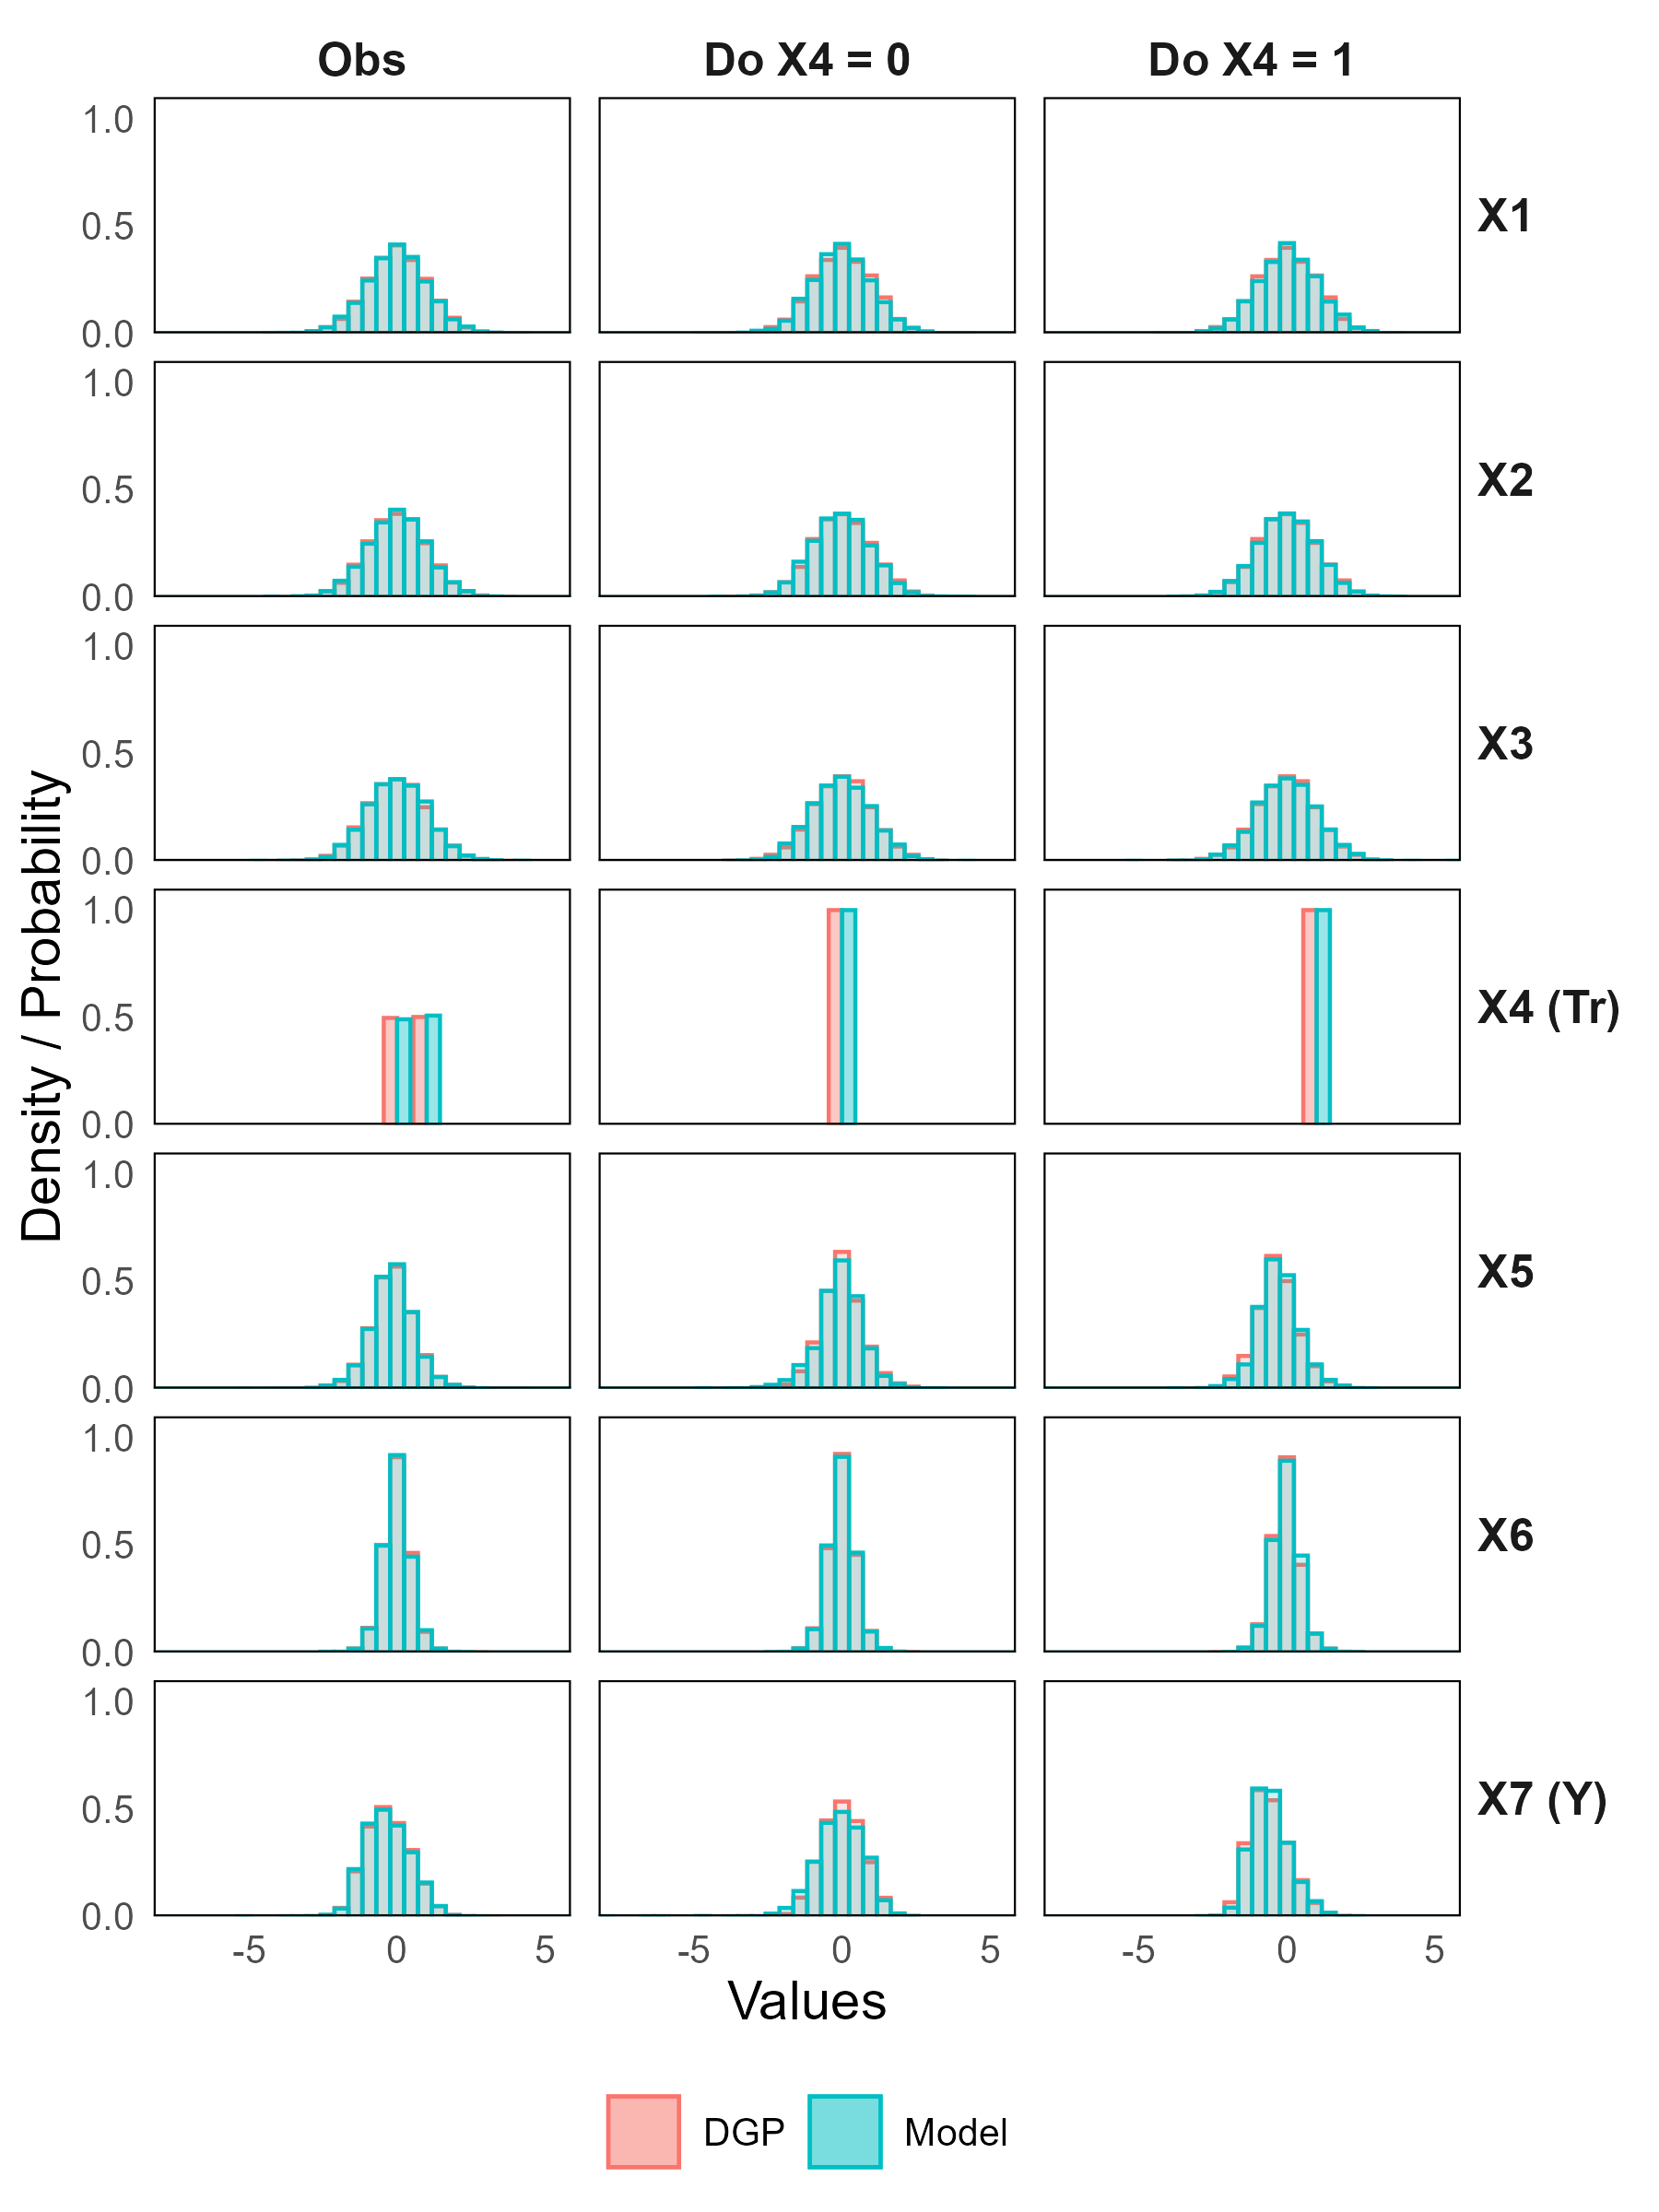
\includegraphics[width=0.45\textwidth]{img/results/rct_scenario2_sampling_distributions_vertical.png}
\caption{Marginal distributions of DGP variables and fitted TRAM-DAG samples for scenario (2), including a direct treatment but no interaction effects. The distributions shown as observed (Obs), under control intervention (Do $X4=0$) and under treatment intervention (Do $X4=1$). Left: Observational; Right: RCT setting.}
\label{fig:scenario2_sampling_distributions_vertical}
\end{figure}

\begin{figure}[htbp]
\centering
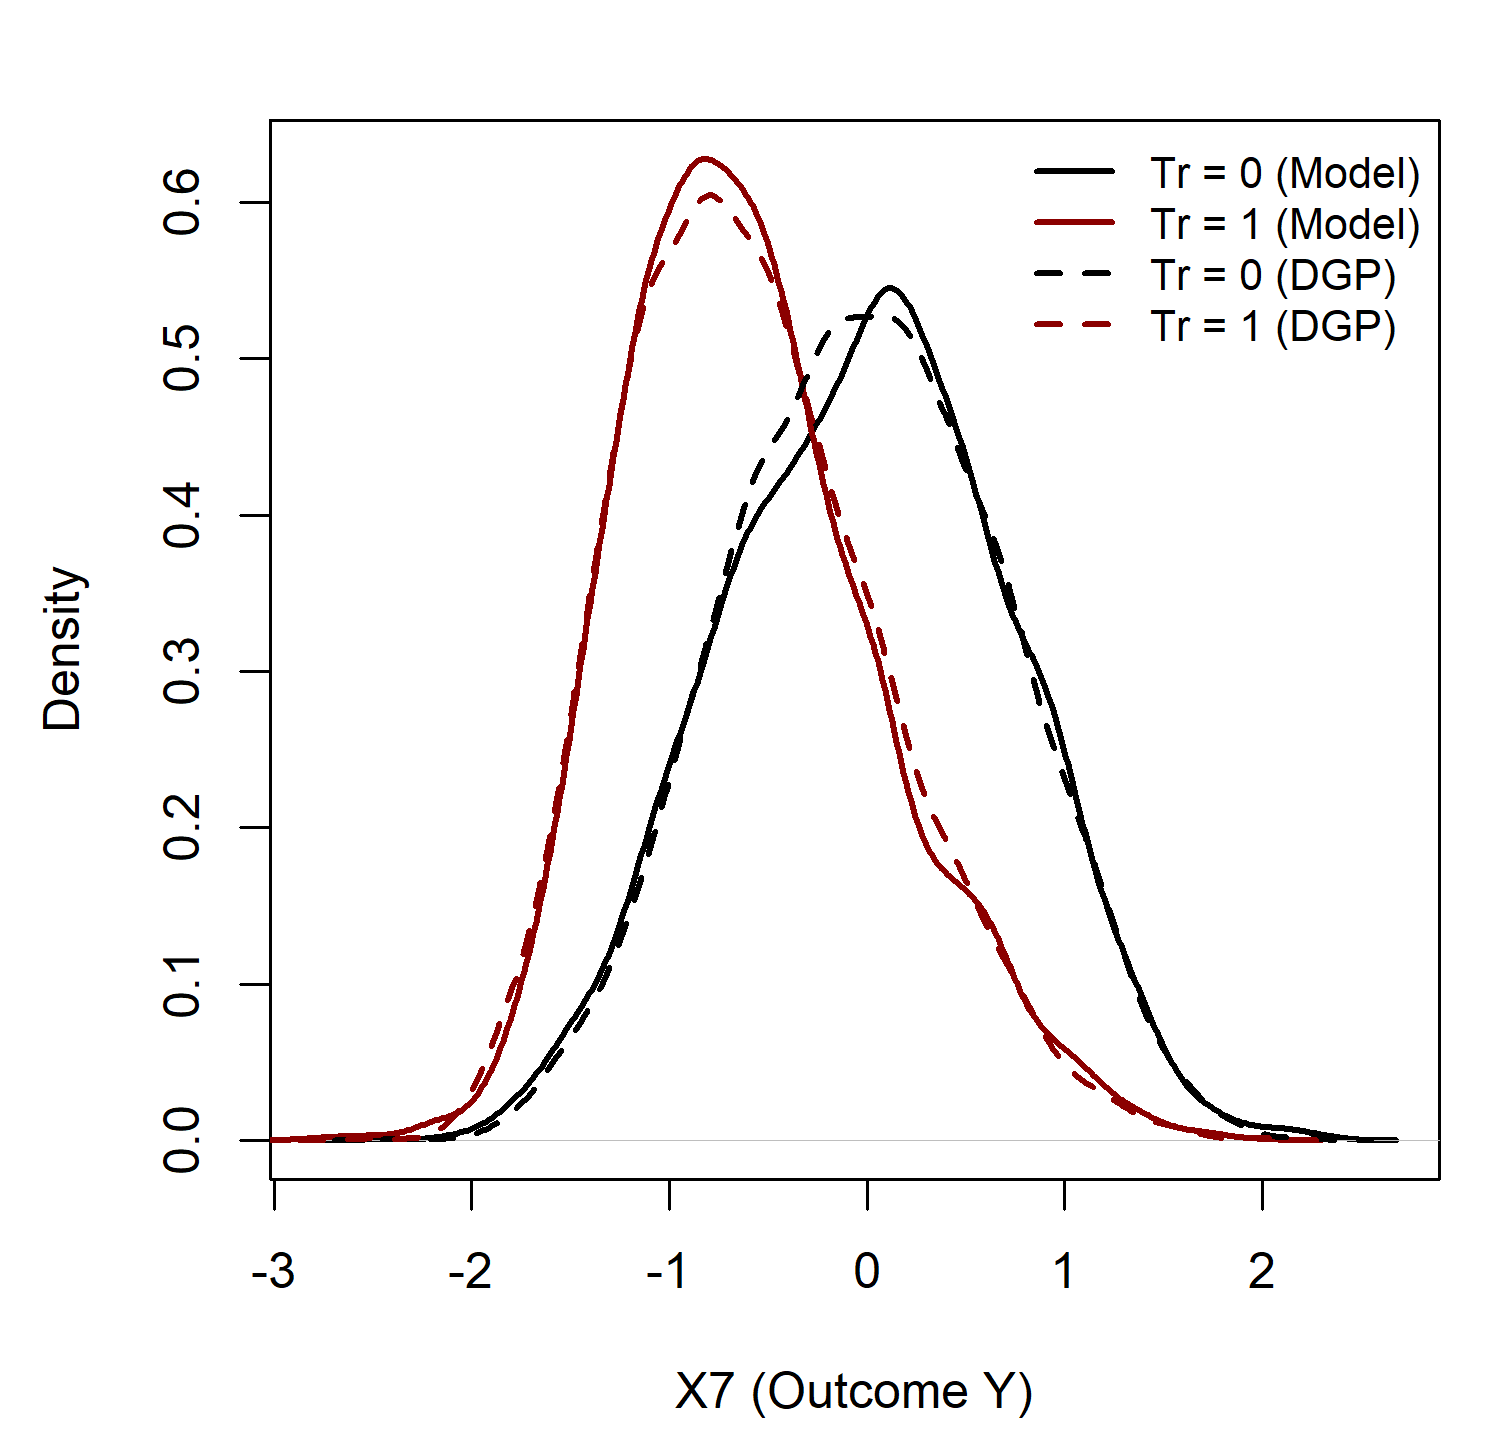
\includegraphics[width=0.45\textwidth]{img/results/observ_scenario2_X7_treatment_densities.png}
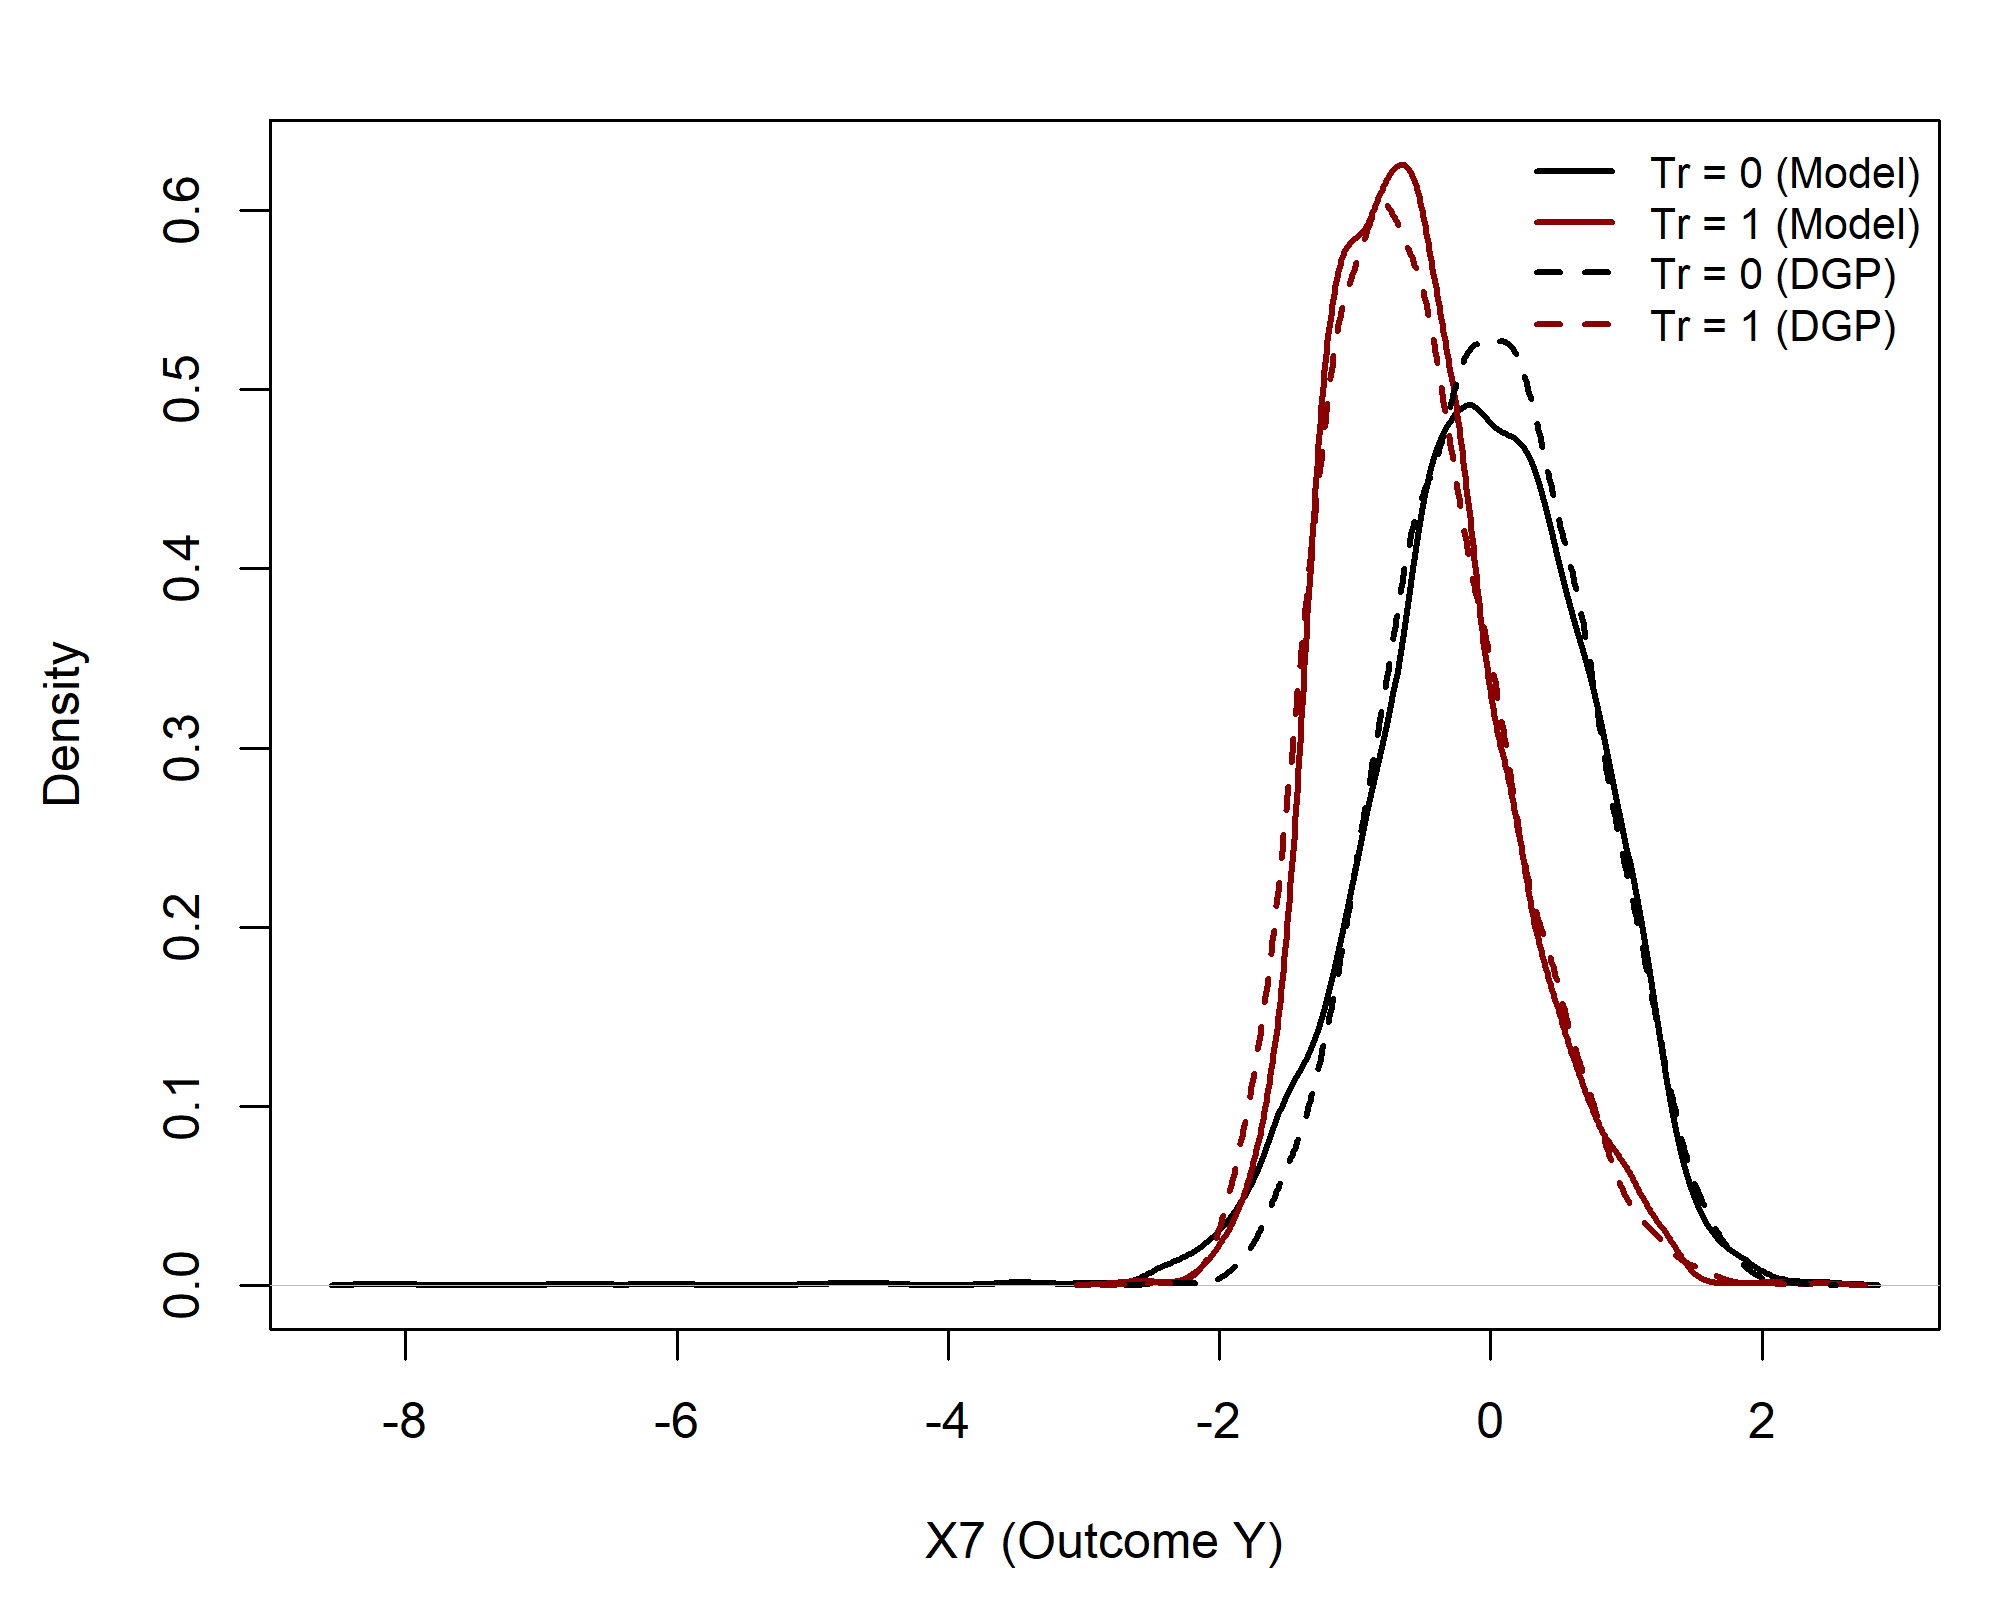
\includegraphics[width=0.45\textwidth]{img/results/rct_scenario2_X7_treatment_densities.png}
\caption{Distributions of the outcome variable (X7) under treatment and control interventions for scenario (2), including a direct treatment but no interaction effects. This plot is a higher resolution view of the X7 panels (Do $X4=0$) and (Do $X4=1$) from Figure \ref{fig:scenario2_sampling_distributions_vertical}. Left: Observational; Right: RCT setting.}
\label{fig:scenario2_outcome_distributions}
\end{figure}




\begin{figure}[htbp]
\centering
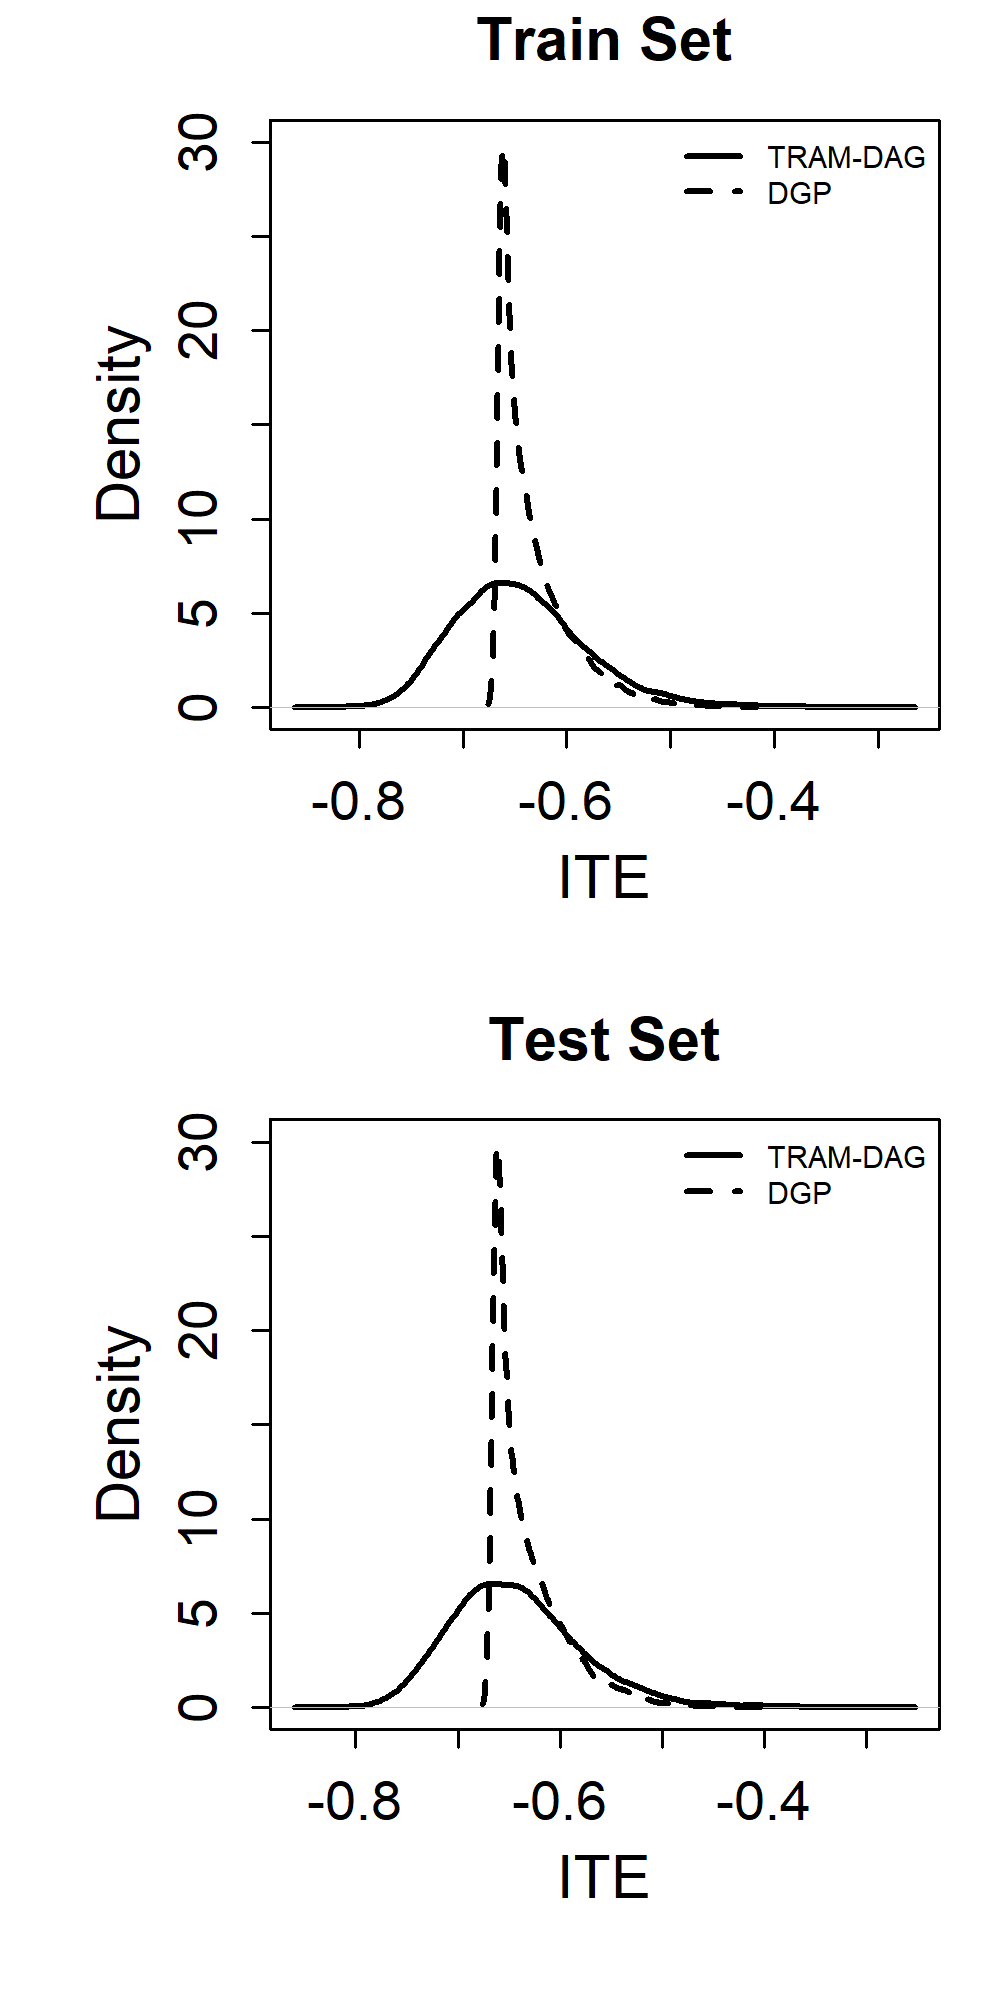
\includegraphics[width=0.45\textwidth]{img/results/observ_scenario2_ITE_densities_train_test.png}
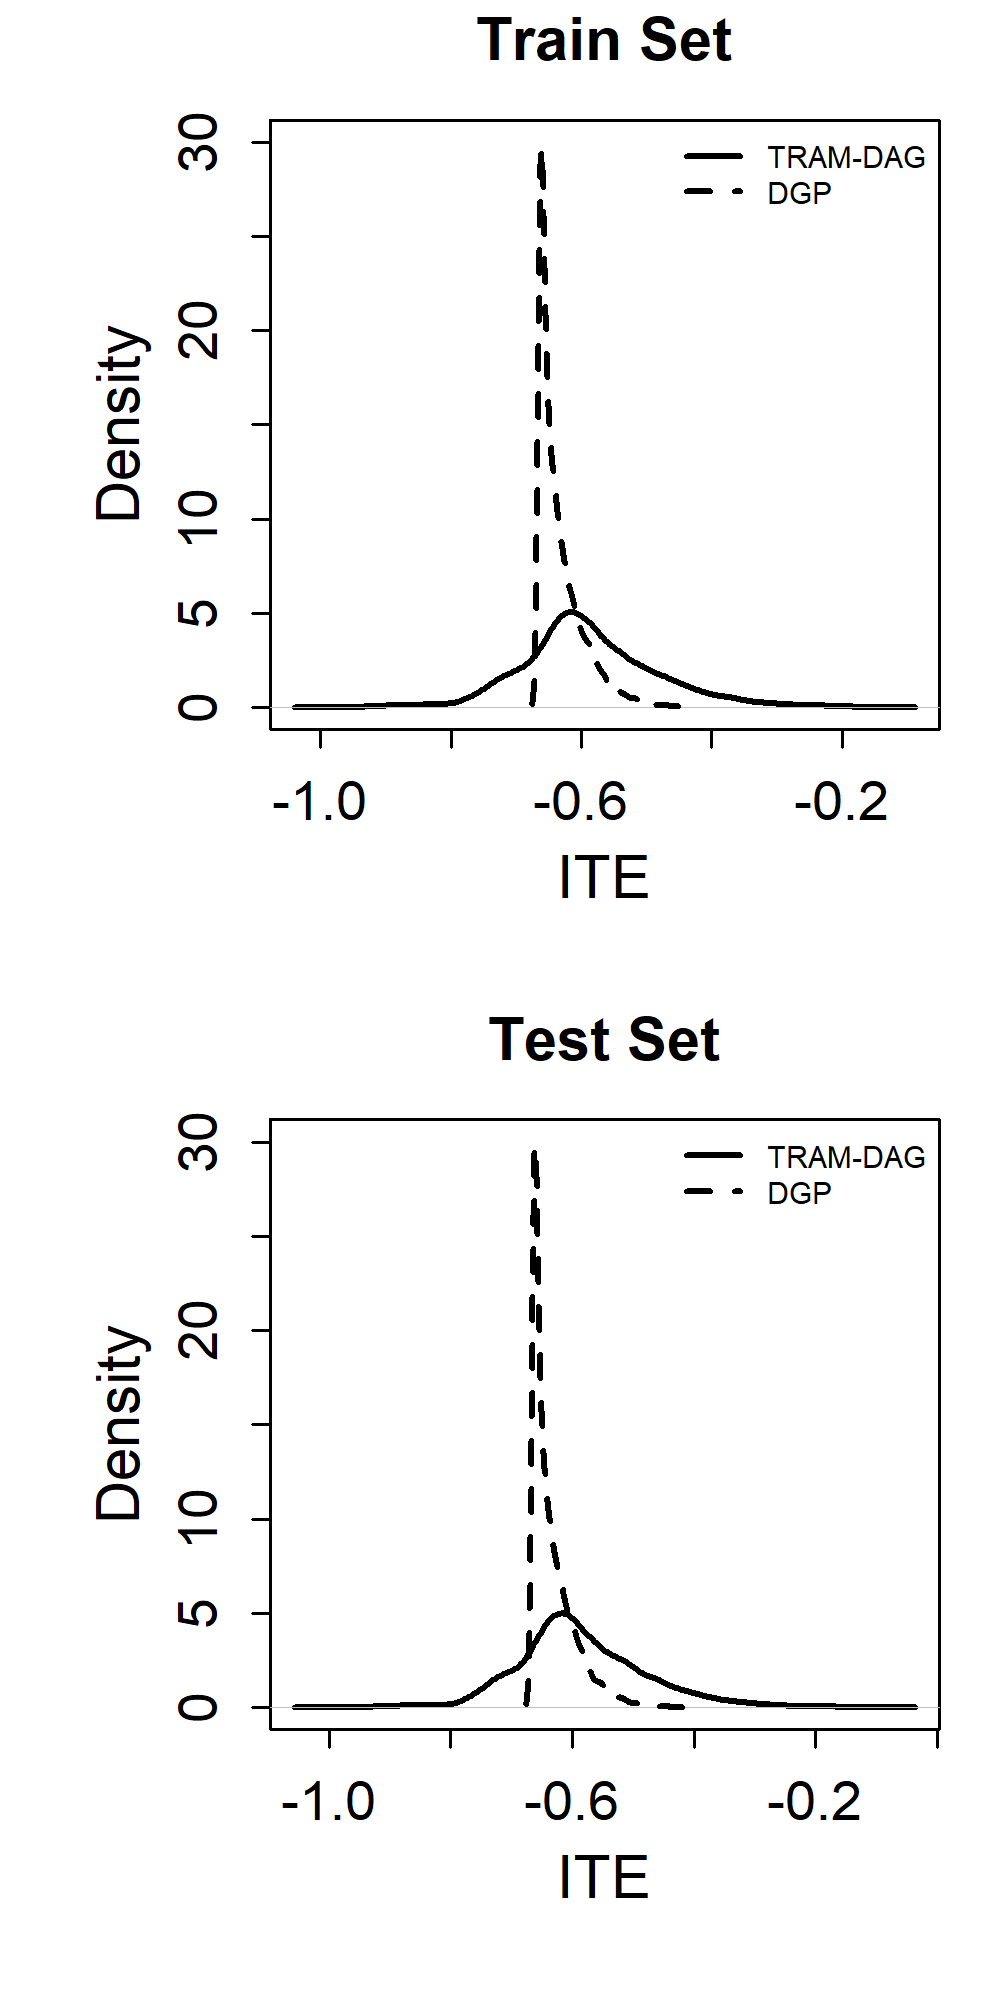
\includegraphics[width=0.45\textwidth]{img/results/rct_scenario2_ITE_densities_train_test.png}
\caption{Densities of estimated ITEs compared to the true ITEs in the training and test datasets for scenario (2), including a direct treatment but no interaction effects. Left: Observational; right: RCT setting.}
\label{fig:scenario2_ite_densities_train_test}
\end{figure}






\begin{figure}[htbp]
\centering
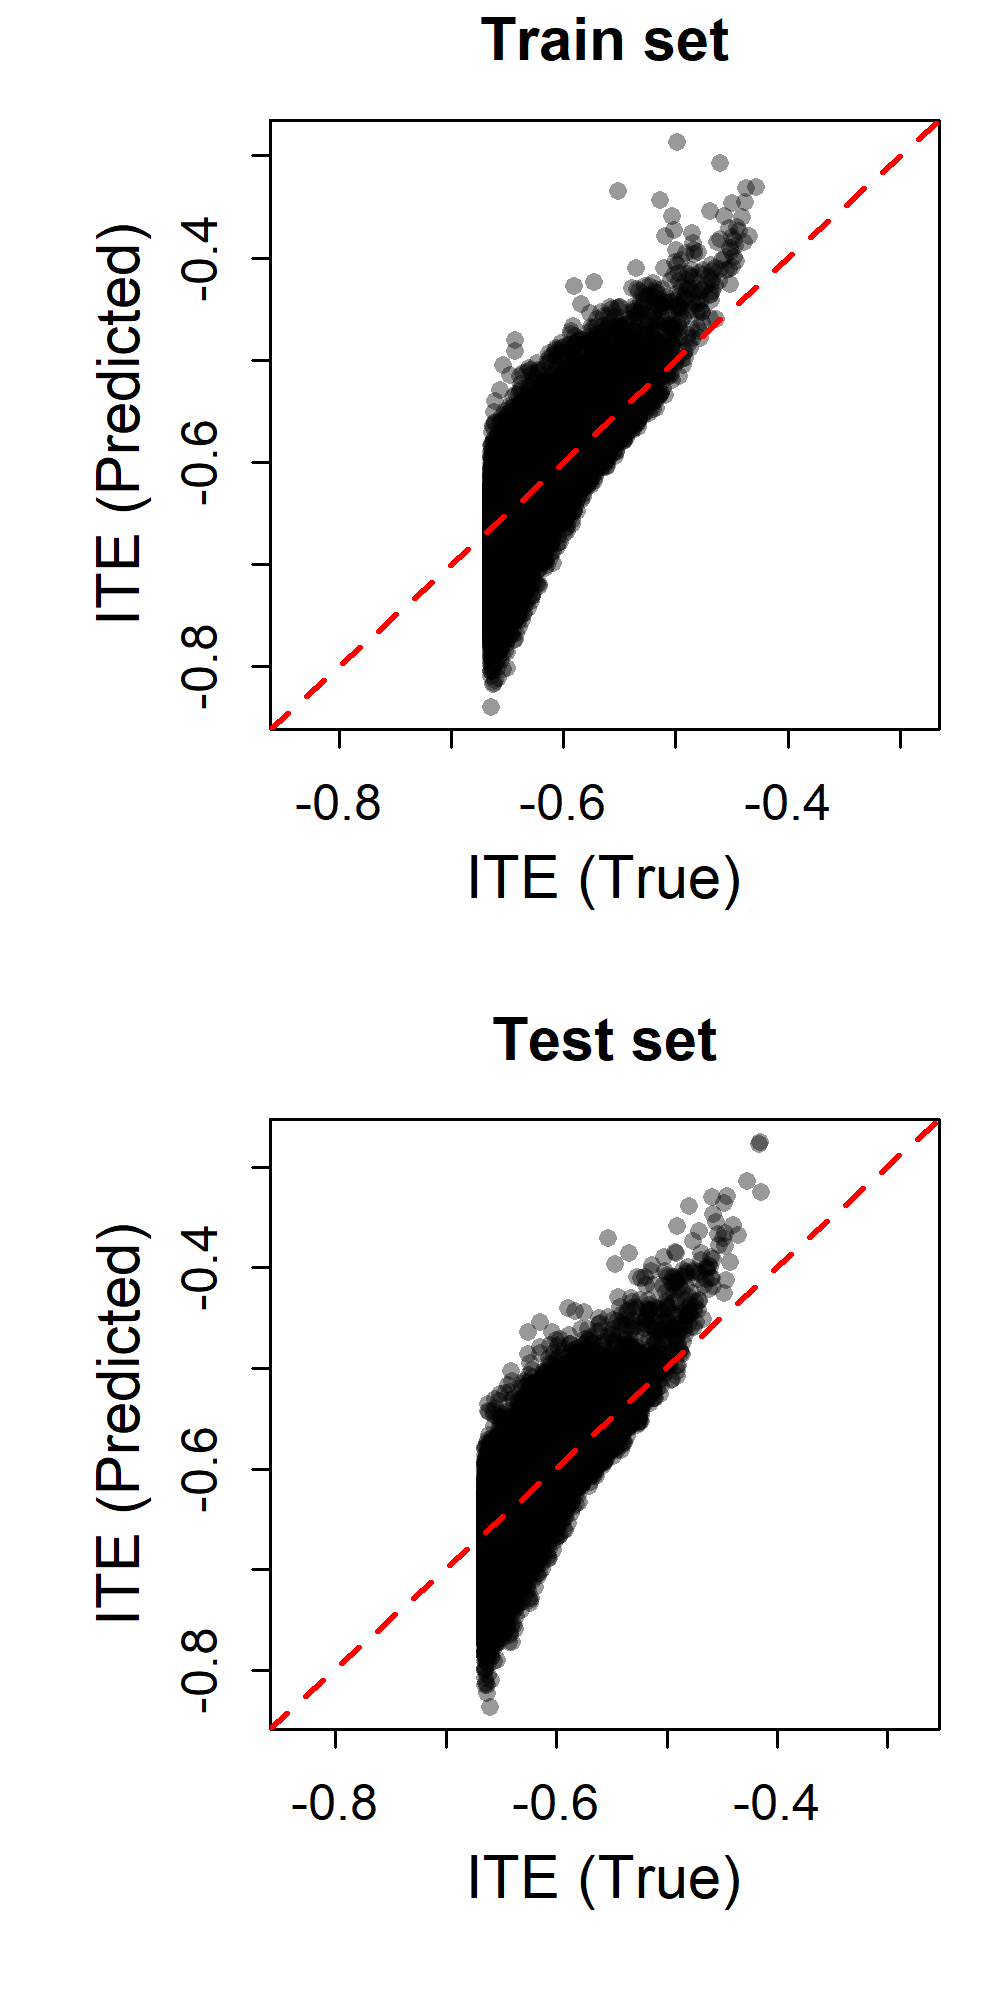
\includegraphics[width=0.45\textwidth]{img/results/observ_scenario2_ITE_scatter_train_test.png}
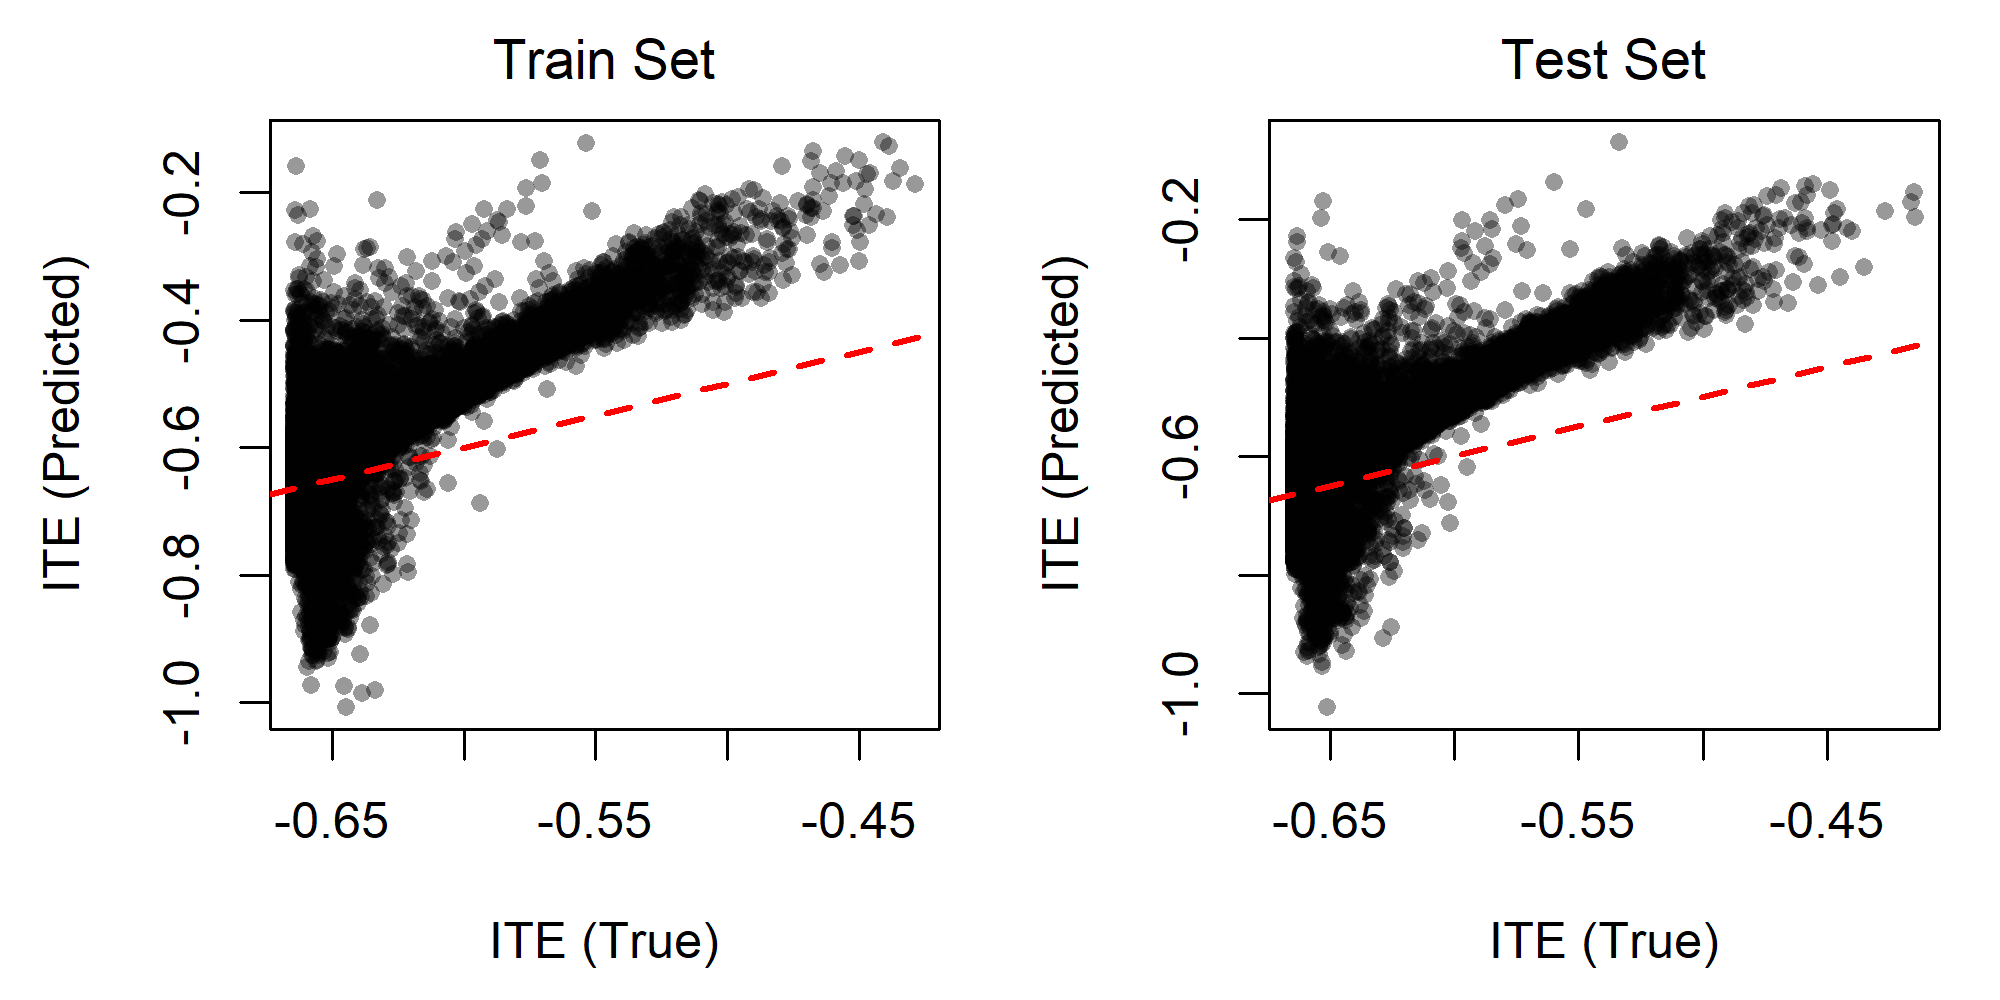
\includegraphics[width=0.45\textwidth]{img/results/rct_scenario2_ITE_scatter_train_test.png}
\caption{Scatterplots of estimated ITEs compared to the true ITEs in the training and test datasets for scenario (2), including a direct treatment but no interaction effects. Left: Observational; right: RCT setting.}
\label{fig:scenario2_ite_scatter_train_test}
\end{figure}




\begin{figure}[htbp]
\centering
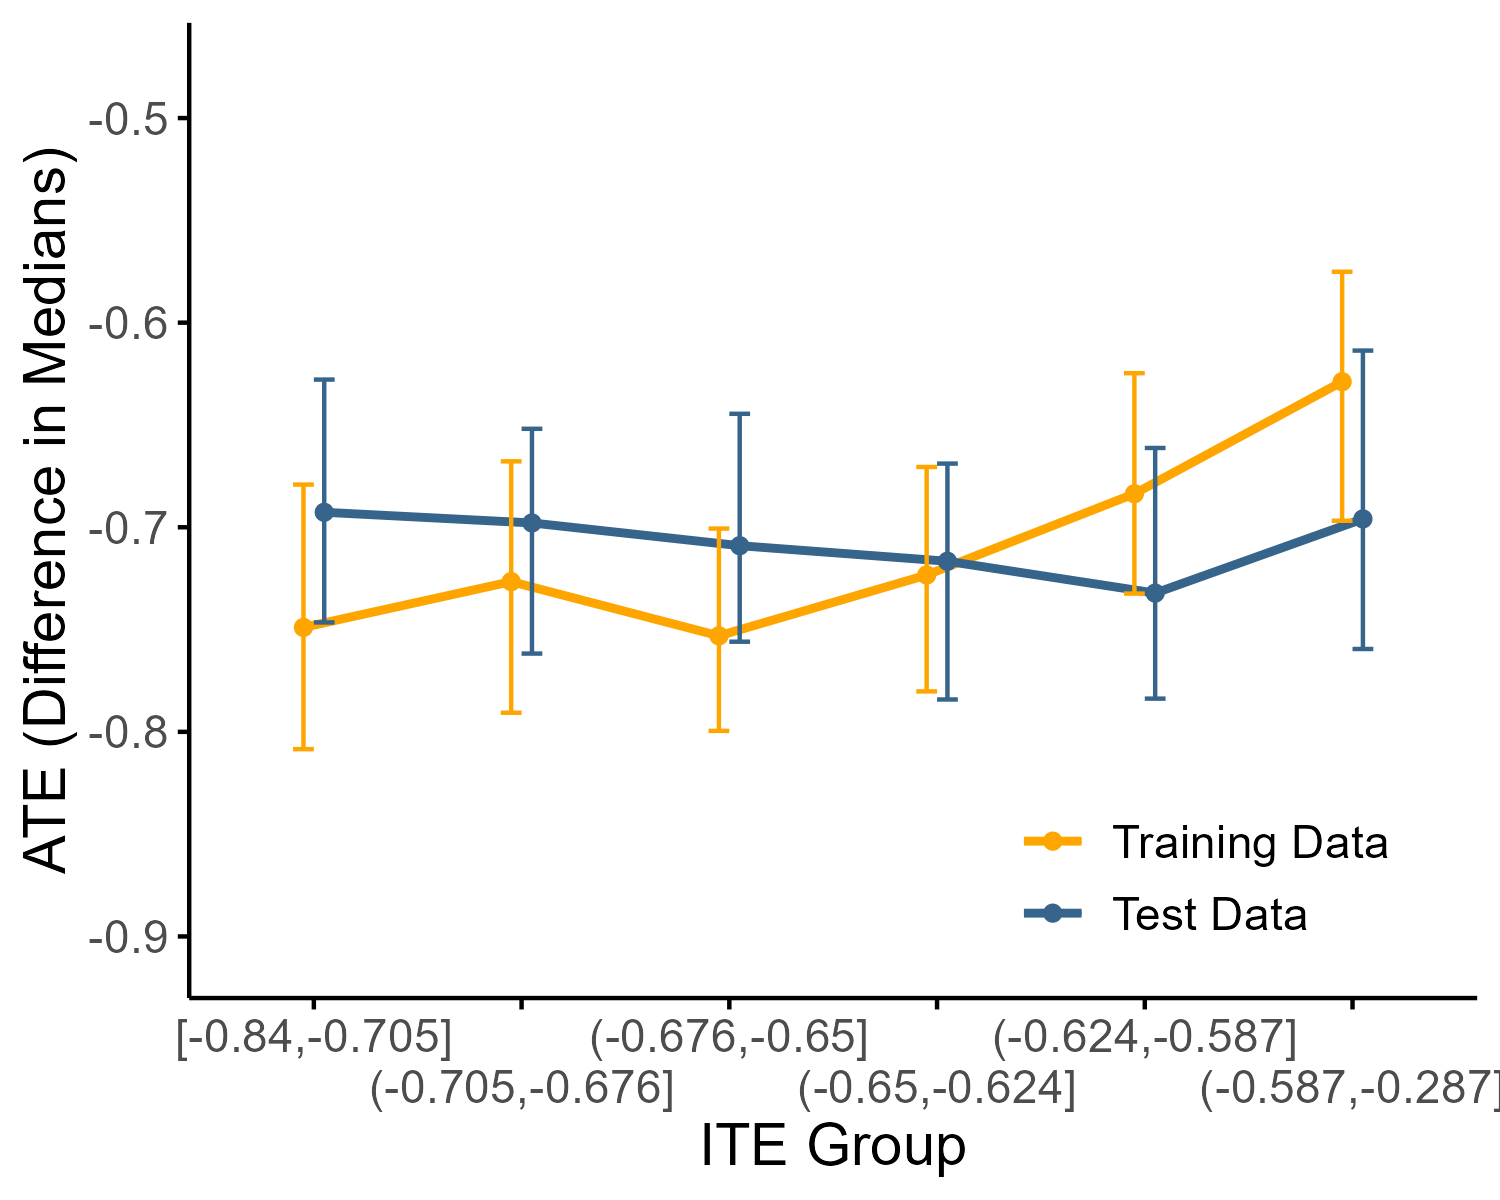
\includegraphics[width=0.45\textwidth]{img/results/observ_scenario2_ITE_cATE.png}
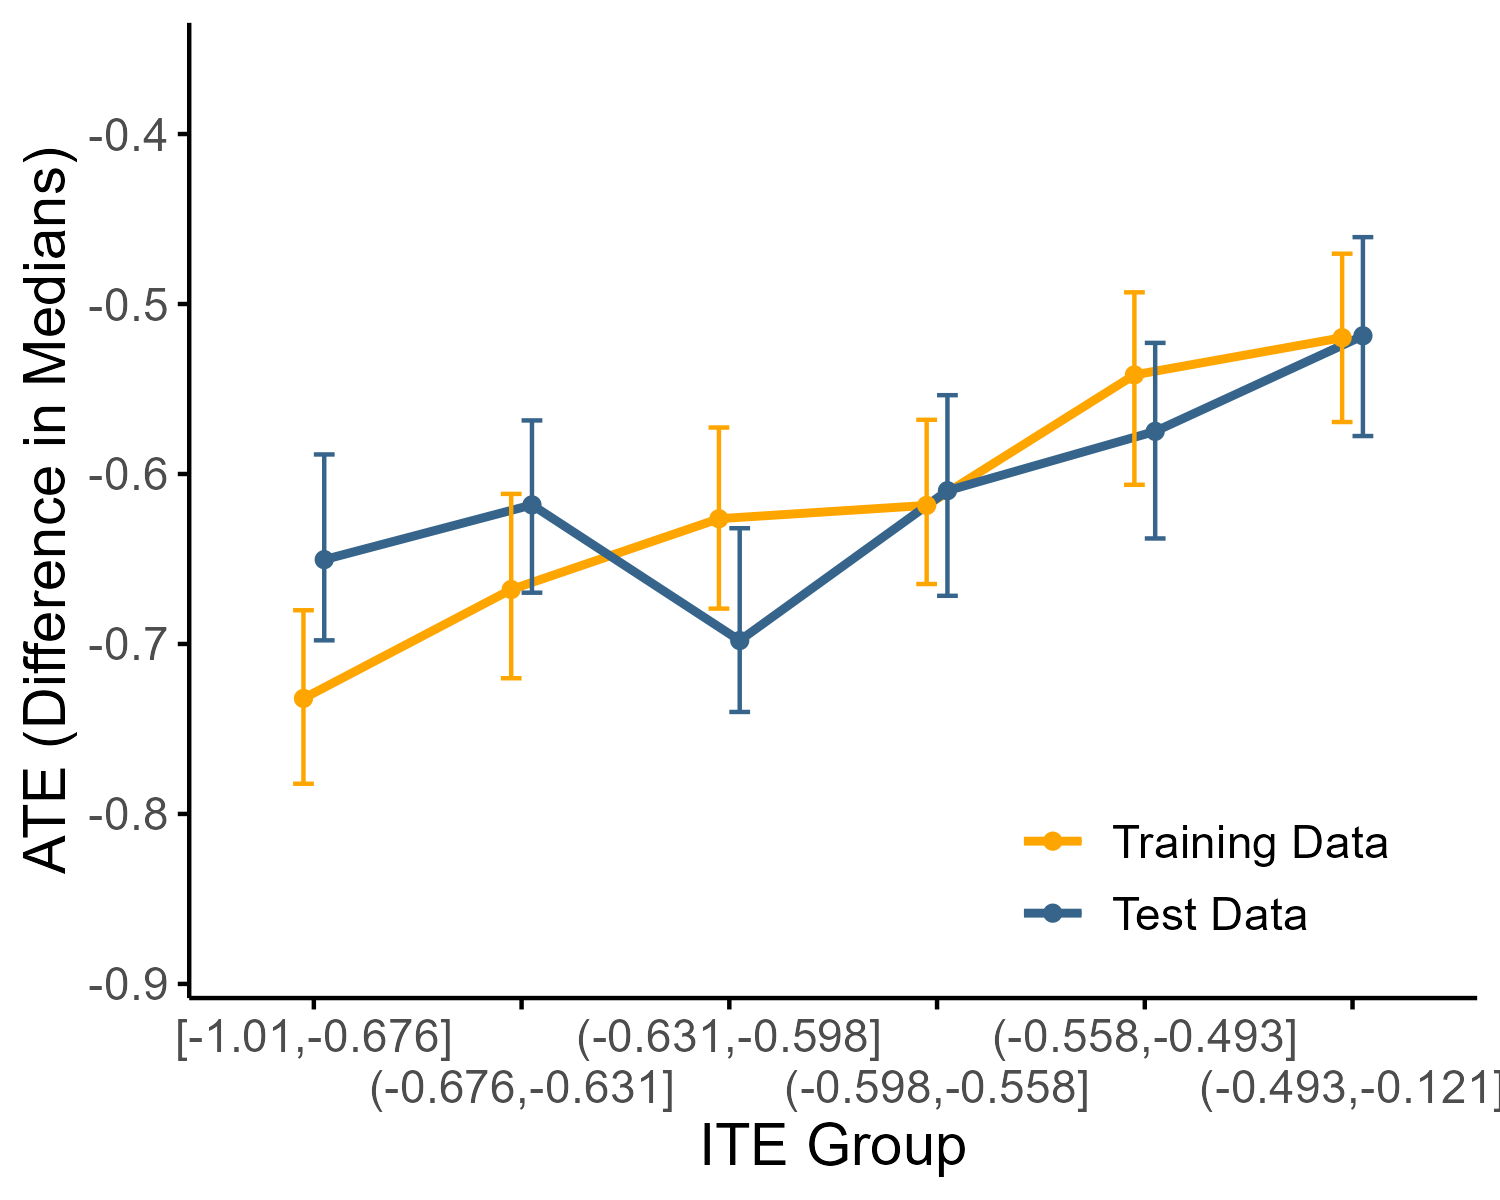
\includegraphics[width=0.45\textwidth]{img/results/rct_scenario2_ITE_cATE.png}
\caption{ITE-ATE plot for scenario (2), including a direct treatment but no interaction effects. Individuals are grouped into bins according to the estimated ITE and in each bin the ATE is calculated as the difference in medians of the observed outcomes under the treatments. 95\% bootstrap confidence intervals indicate the uncertainty. Left: Observational; right: RCT setting.}
\label{fig:scenario2_ite_cATE}
\end{figure}



\clearpage 
¨
\subsection{Scenario (3): No direct but with interaction effects}

Scenario (3) included no direct effect of the treatment on the outcome but it included interaction effects of the treatment with the covariates X2 and X3. Compared to scenario (1), when excluding the direct effect of the treatment, the distribution of ITEs is more centered as shown in Figure \ref{fig:scenario3_ite_distribution_dgp}. The ATE in terms of the mean difference in the test set of the RCT setting is $-0.048$ with a confidence interval of $-0.068$ to $-0.028$. 



\begin{table}[htbp]
\centering
\small
\caption{Scenario (3), without direct treatment effect but including interaction effects: Comparison of ATE measures across train and test sets for the observational and RCT setting.}
\label{tab:scenario3_ate_comparison}
\begin{tabular}{l c c c c}
\toprule
\textbf{Measure} & \multicolumn{2}{c}{\textbf{Observational}} & \multicolumn{2}{c}{\textbf{RCT}} \\
\cmidrule(lr){2-3} \cmidrule(lr){4-5}
 & \textbf{Train} & \textbf{Test} & \textbf{Train} & \textbf{Test} \\
\midrule
ATE as $\text{mean}(\text{Y}_\text{observed}^{(1)}) - \text{mean}(\text{Y}_\text{observed}^{(0)})$ & NA & NA & -0.048 & -0.048 \\
ATE as $\text{median}(\text{Y}_\text{observed}^{(1)}) - \text{median}(\text{Y}_\text{observed}^{(0)})$ & NA & NA & -0.048 & -0.059 \\
ATE as mean(ITE$_\text{true}$)  & -0.065 & -0.068 & -0.065 & -0.068 \\
ATE as mean(ITE$_\text{estimated}$) & -0.059 & -0.061 & -0.051 & -0.053 \\
\bottomrule
\end{tabular}
\end{table}



\begin{figure}[htbp]
\centering
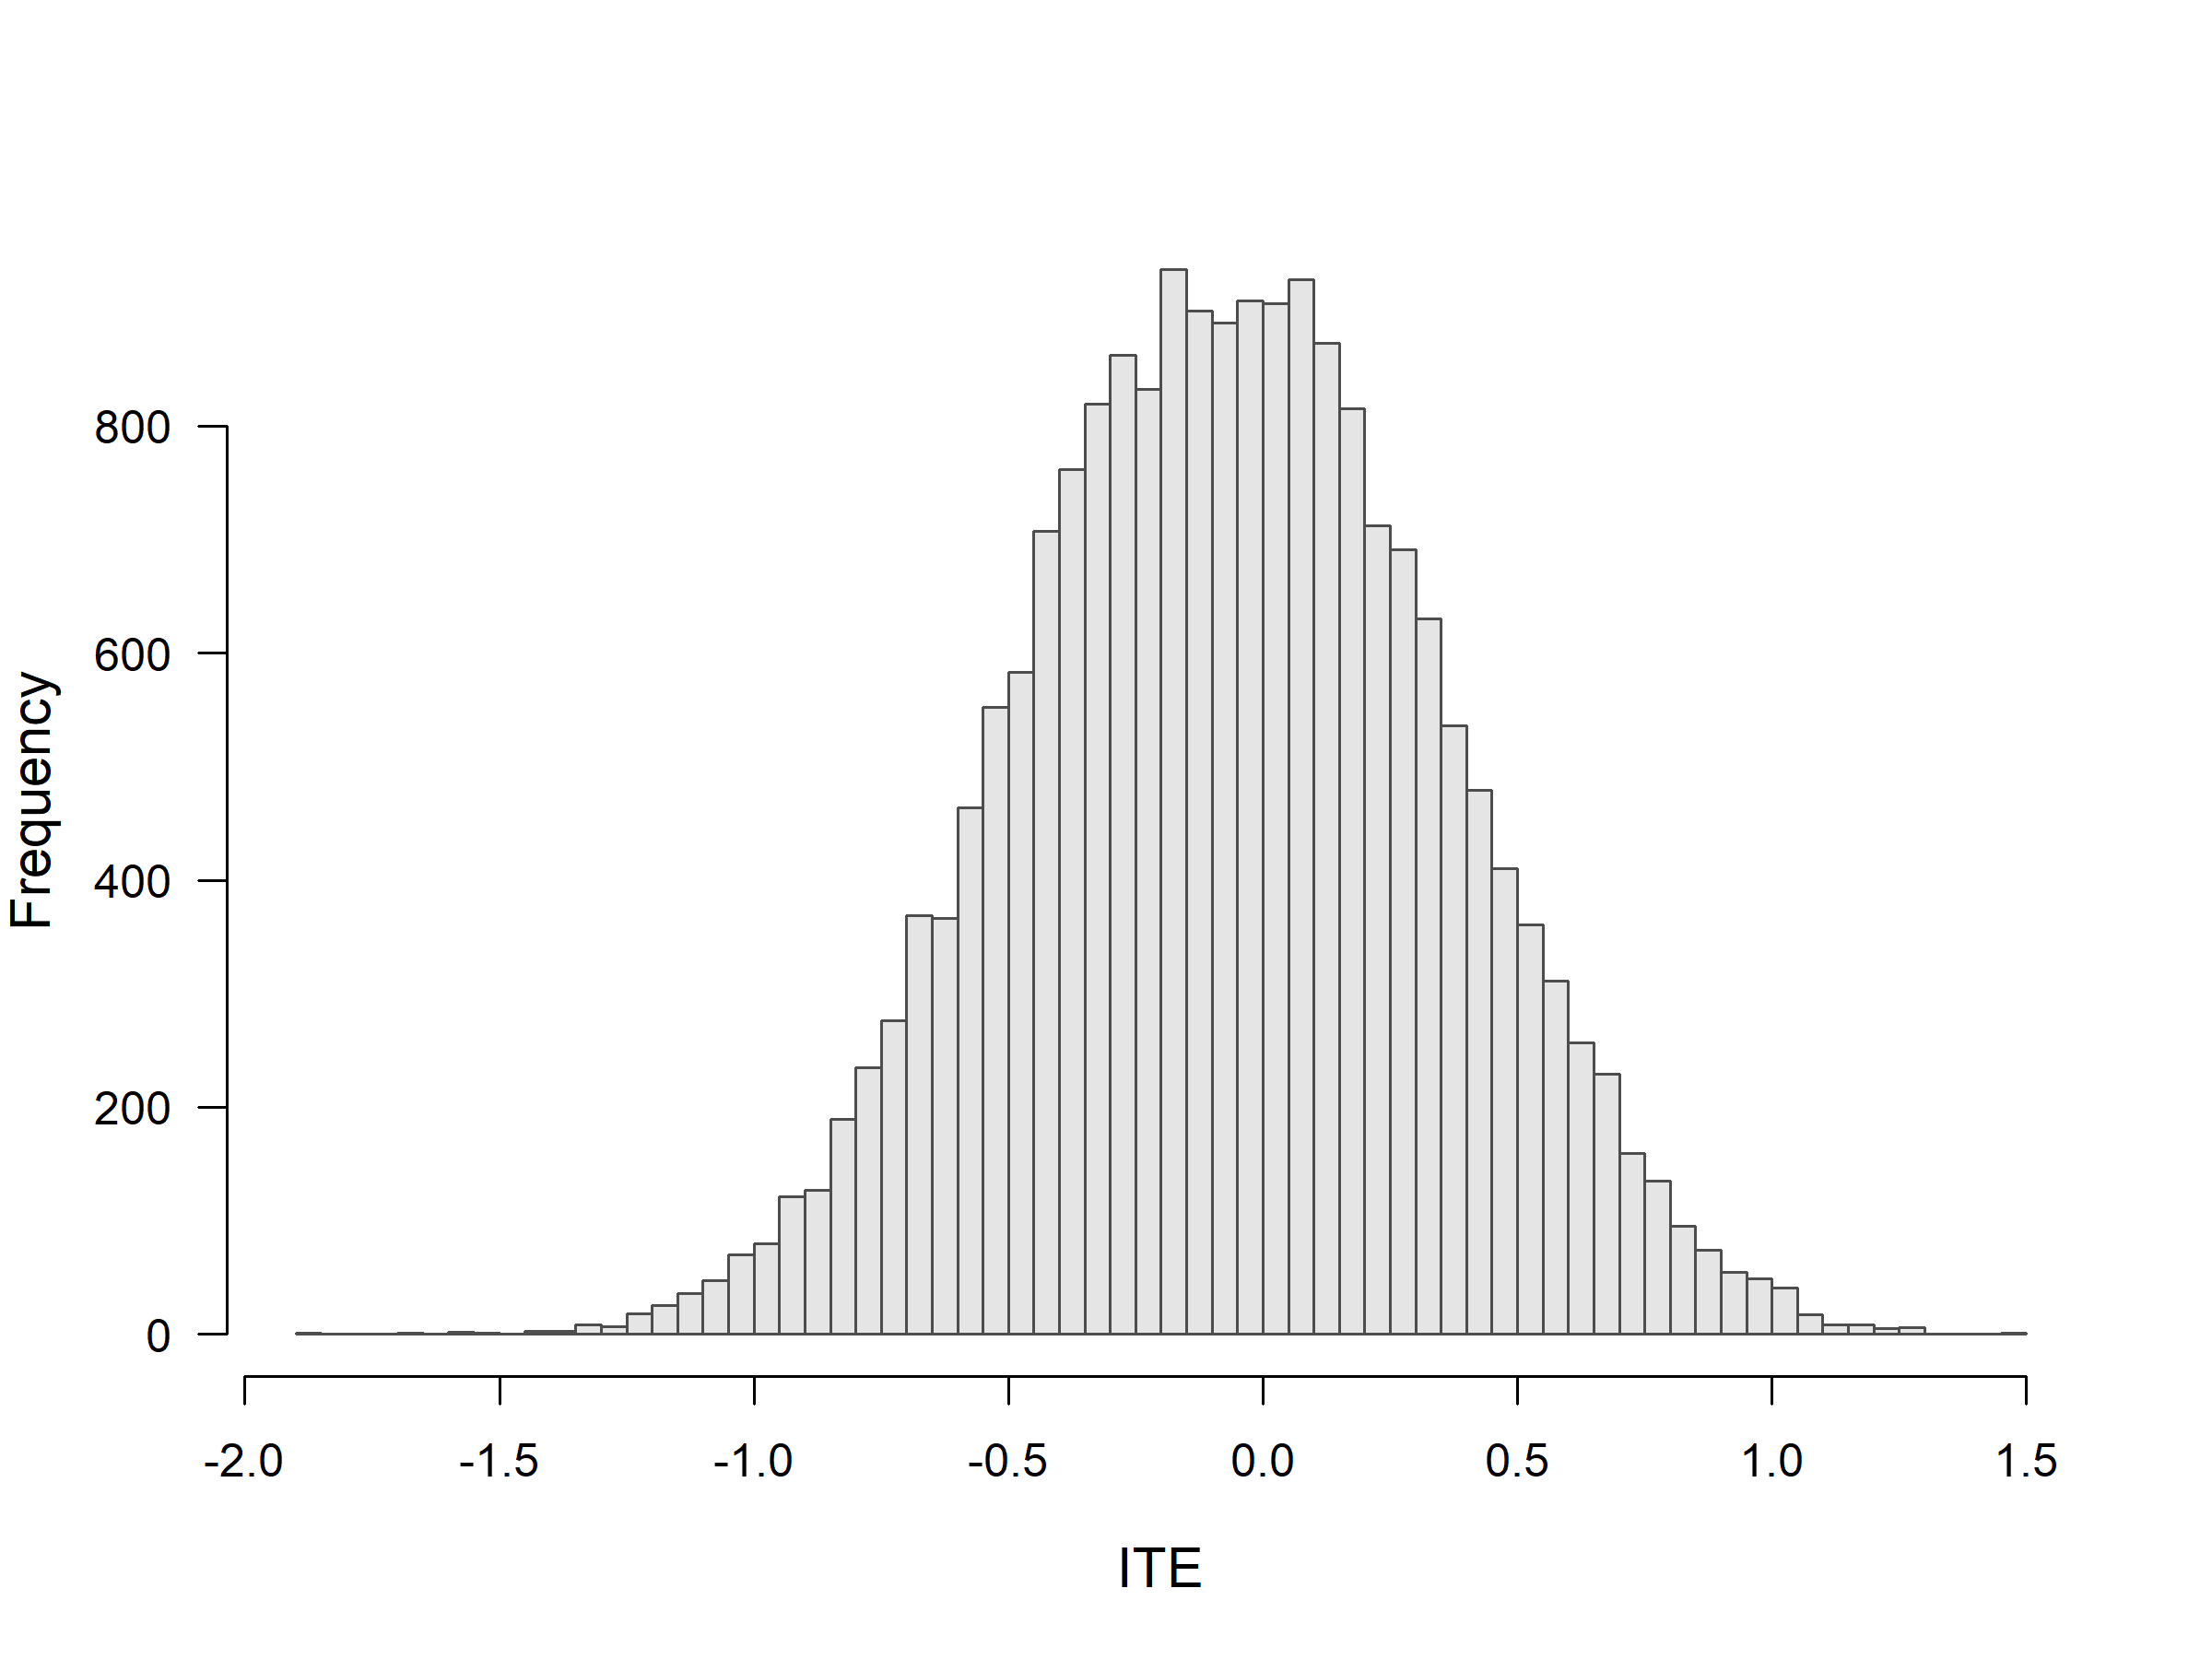
\includegraphics[width=0.45\textwidth]{img/results/observ_scenario3_ite_distribution_dgp.png}
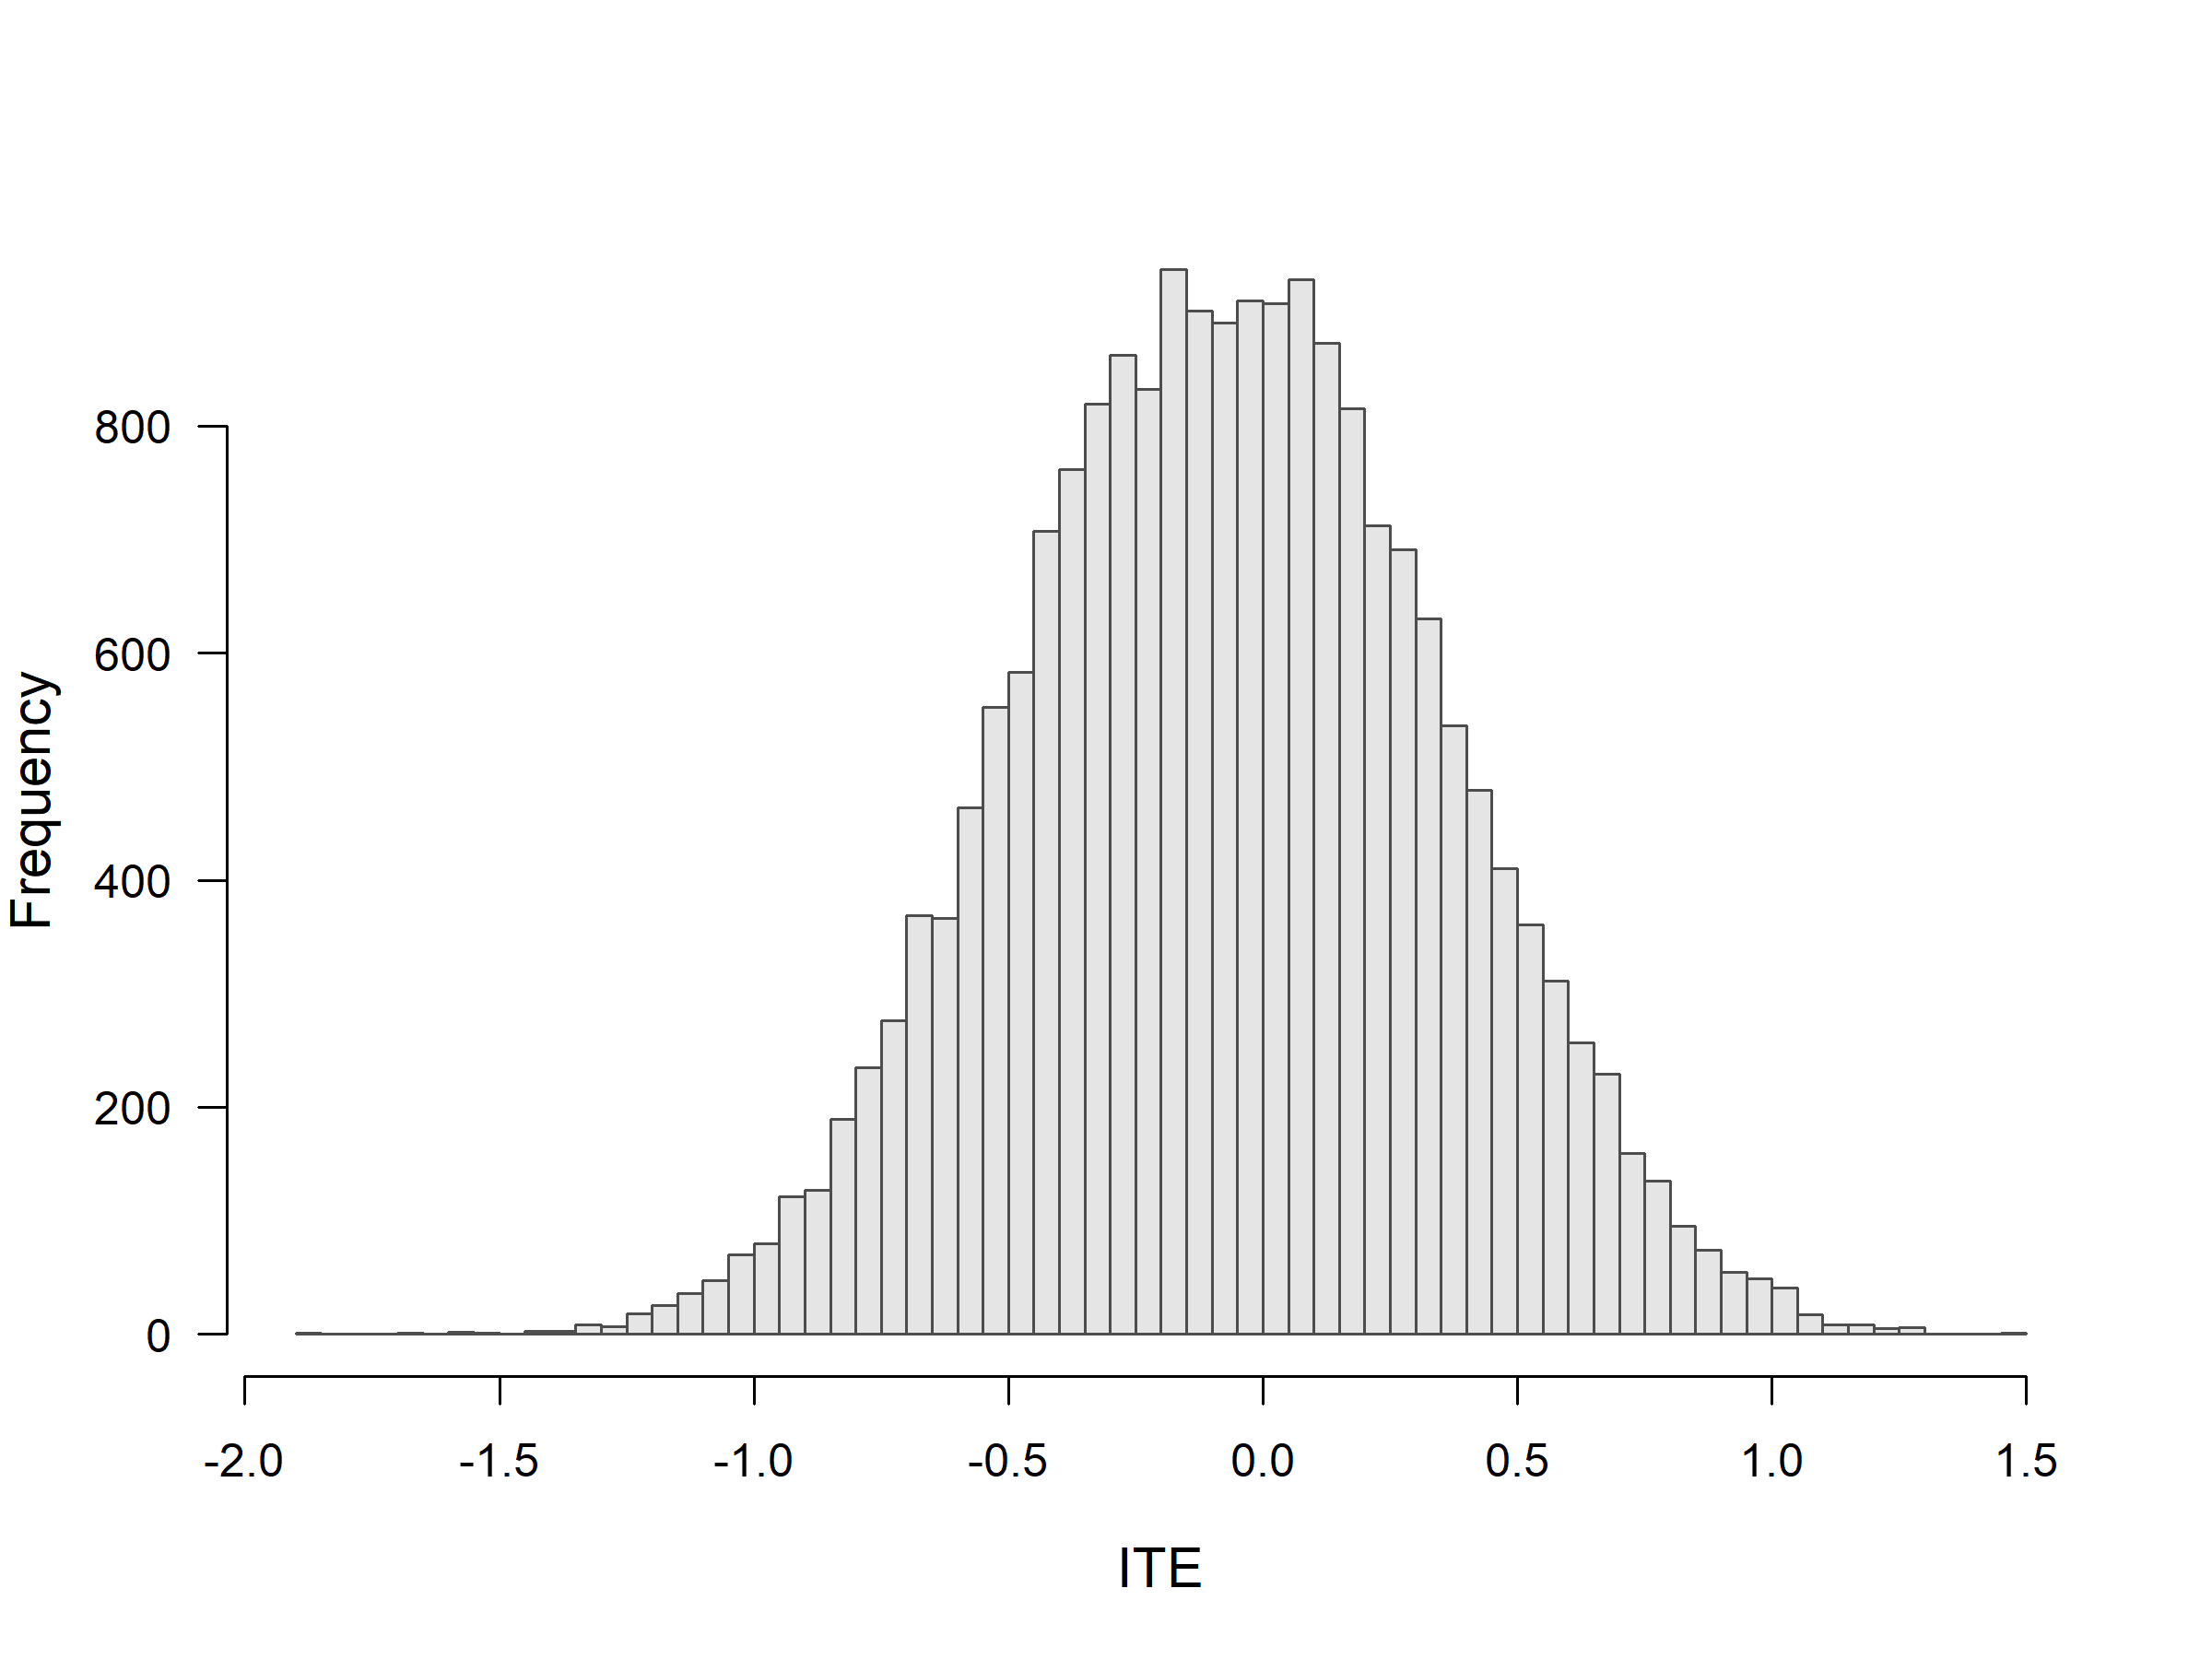
\includegraphics[width=0.45\textwidth]{img/results/rct_scenario3_ite_distribution_dgp.png}
\caption{True ITE distribution resulting from the DGP for scenario (3), without direct treatment effect but including interaction effects. The true ITEs are identical in the observational and in the RCT setting, since they depend on the potential outcomes under both treatment allocations. Left: Observational; Right: RCT setting.}
\label{fig:scenario3_ite_distribution_dgp}
\end{figure}



\begin{figure}[htbp]
\centering
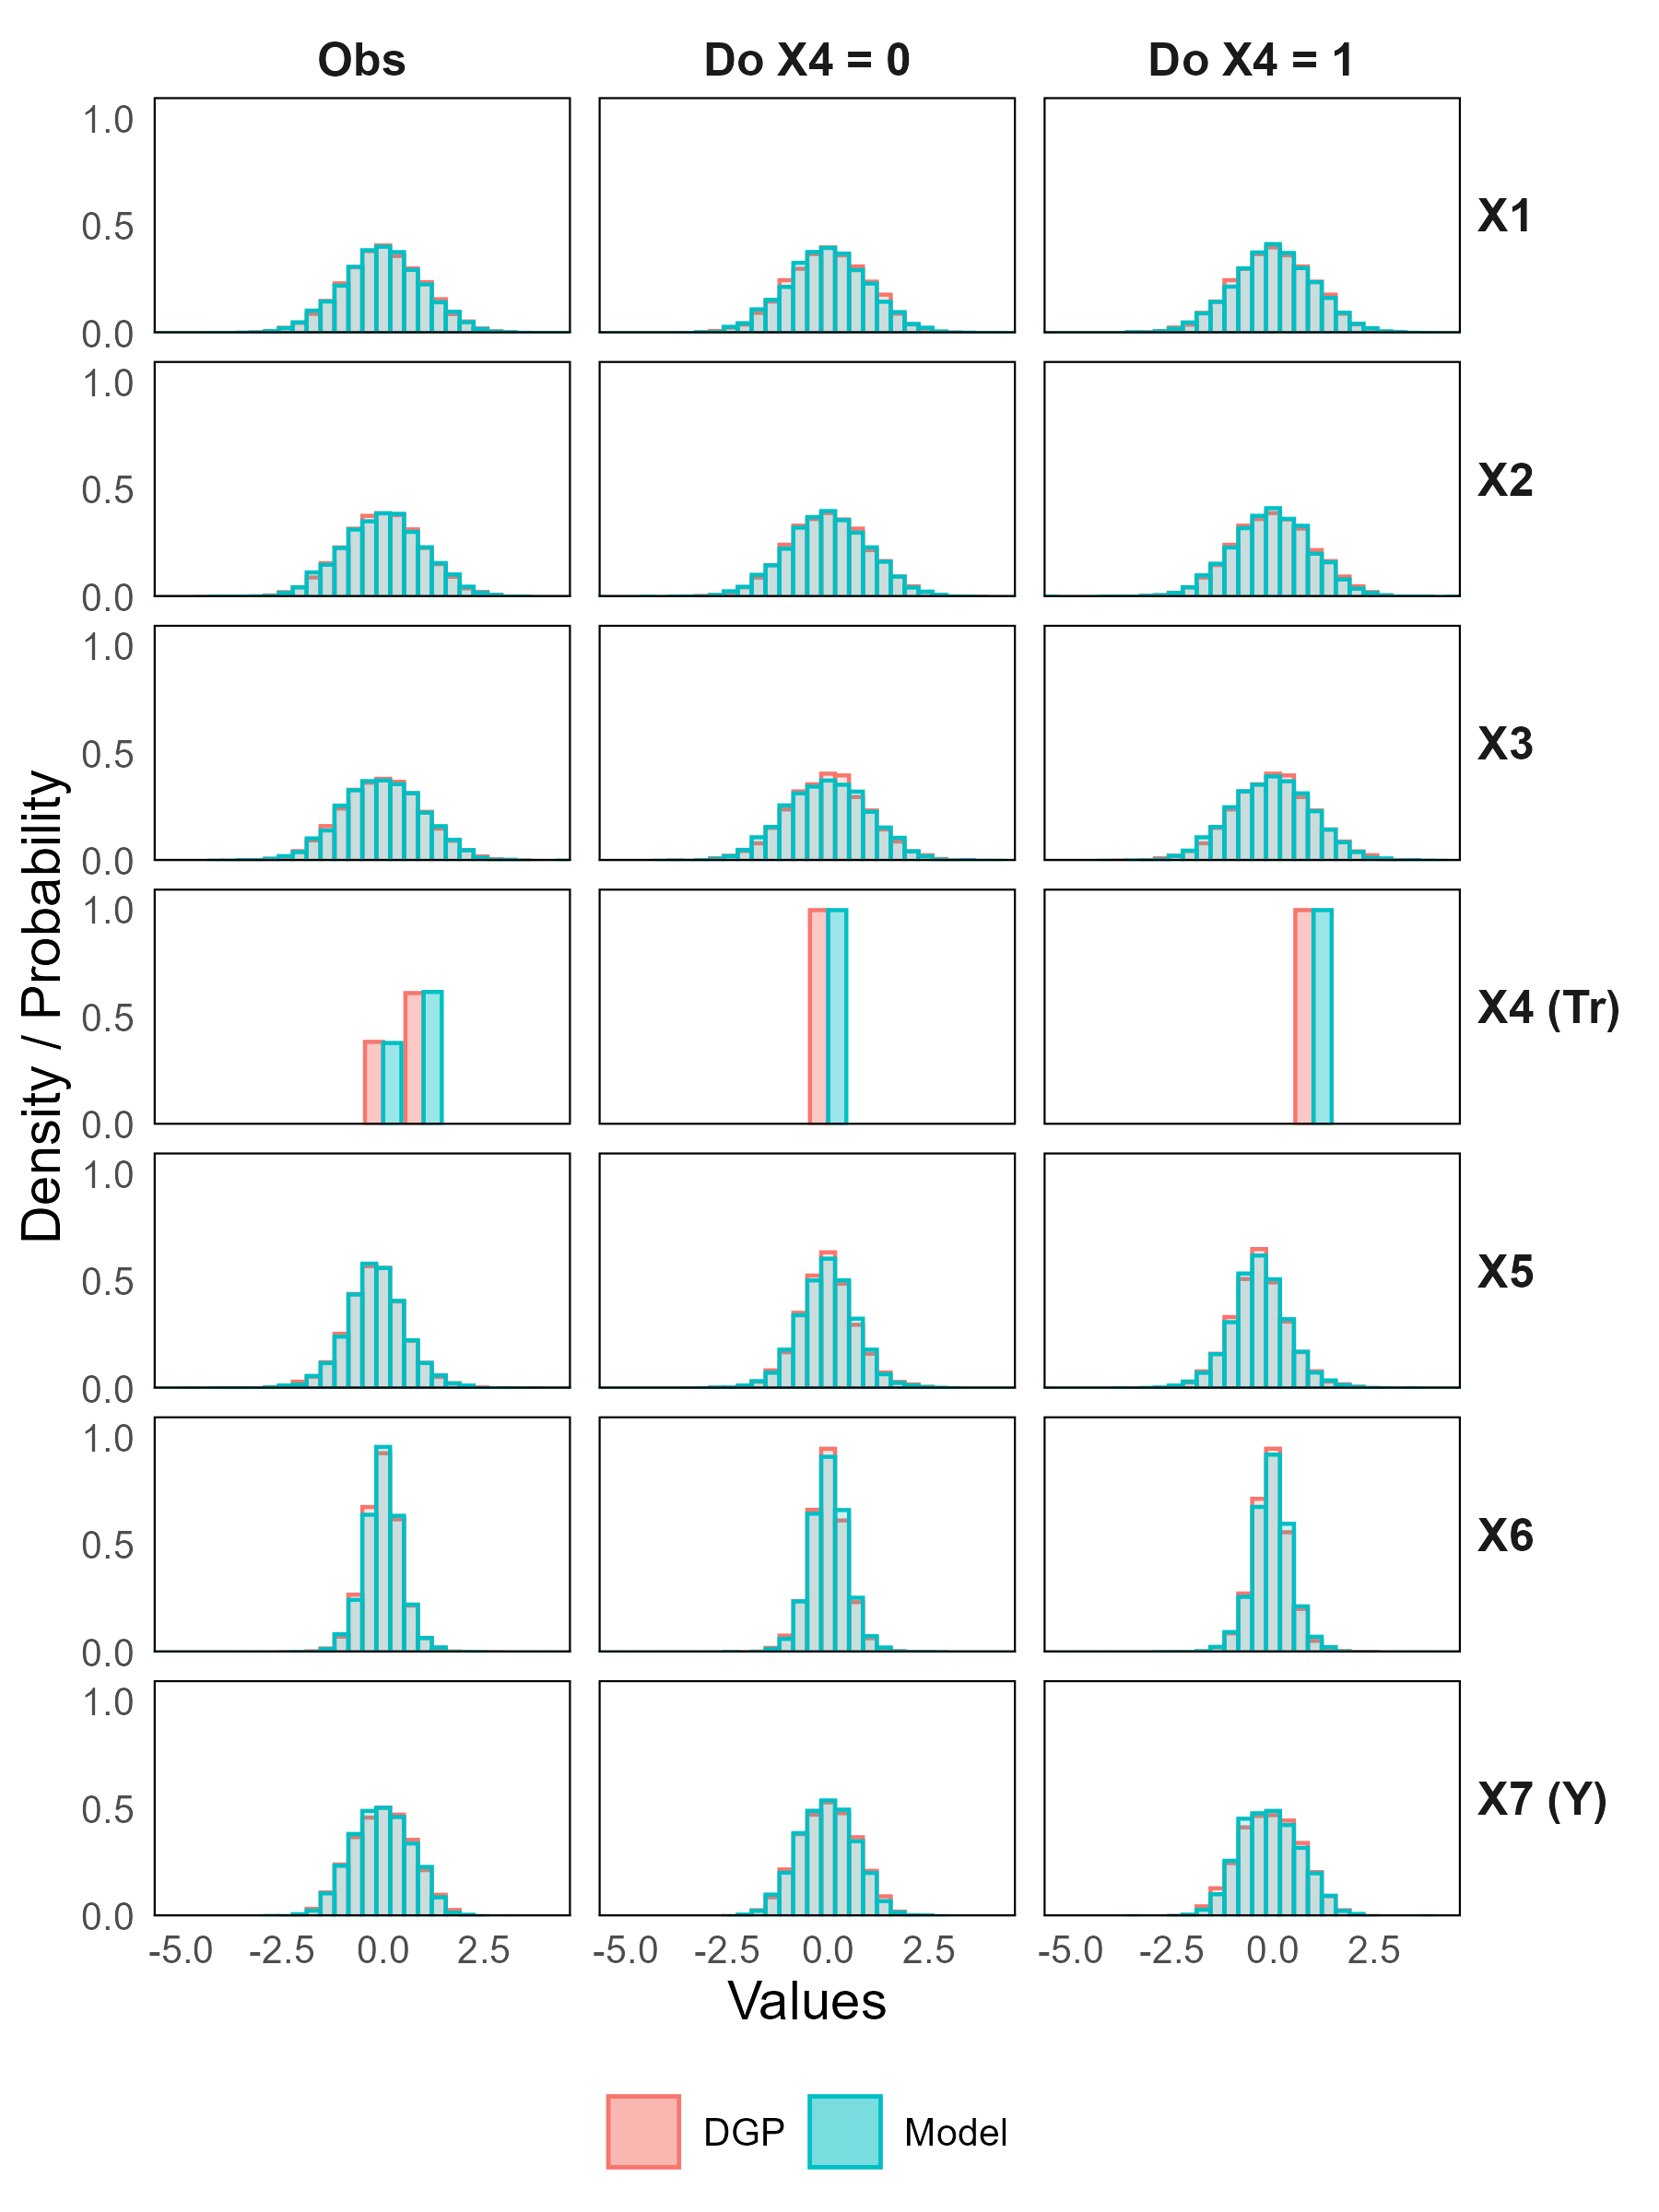
\includegraphics[width=0.45\textwidth]{img/results/observ_scenario3_sampling_distributions_vertical.png}
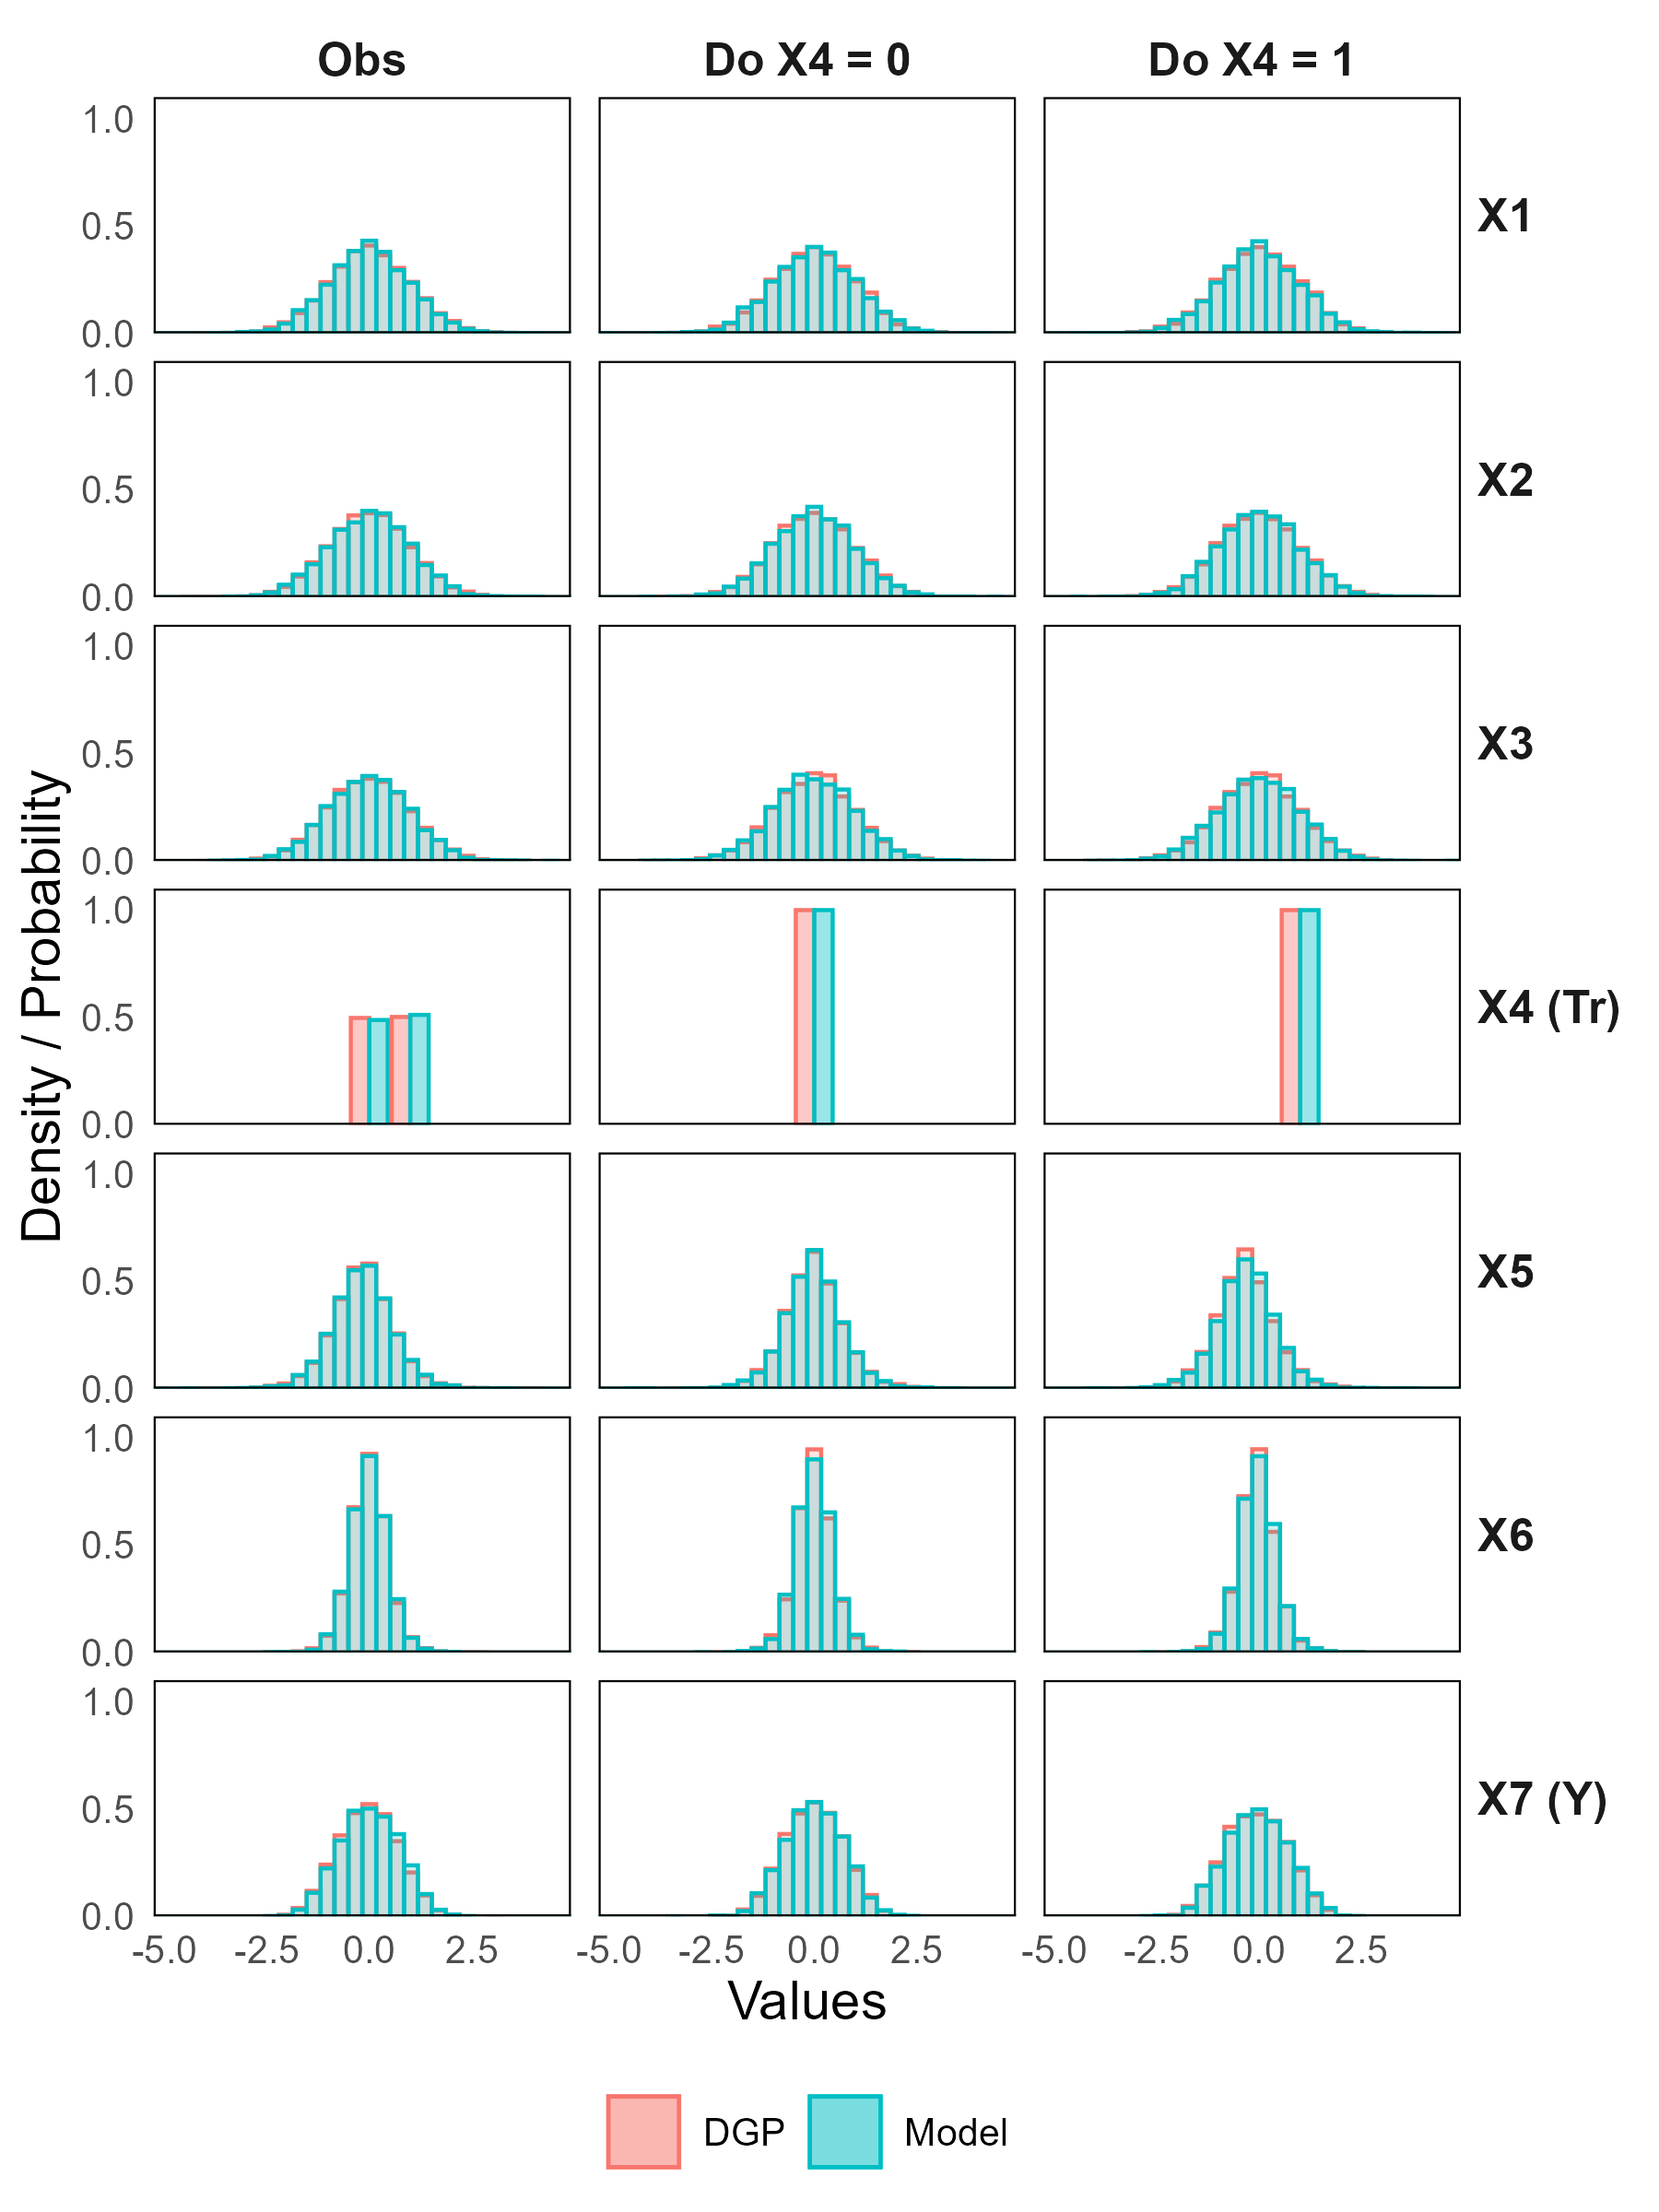
\includegraphics[width=0.45\textwidth]{img/results/rct_scenario3_sampling_distributions_vertical.png}
\caption{Marginal distributions of DGP variables and fitted TRAM-DAG samples for scenario (3), without direct treatment effect but including interaction effects. The distributions shown as observed (Obs), under control intervention (Do $X4=0$) and under treatment intervention (Do $X4=1$). Left: Observational; Right: RCT setting.}
\label{fig:scenario3_sampling_distributions_vertical}
\end{figure}

\begin{figure}[htbp]
\centering
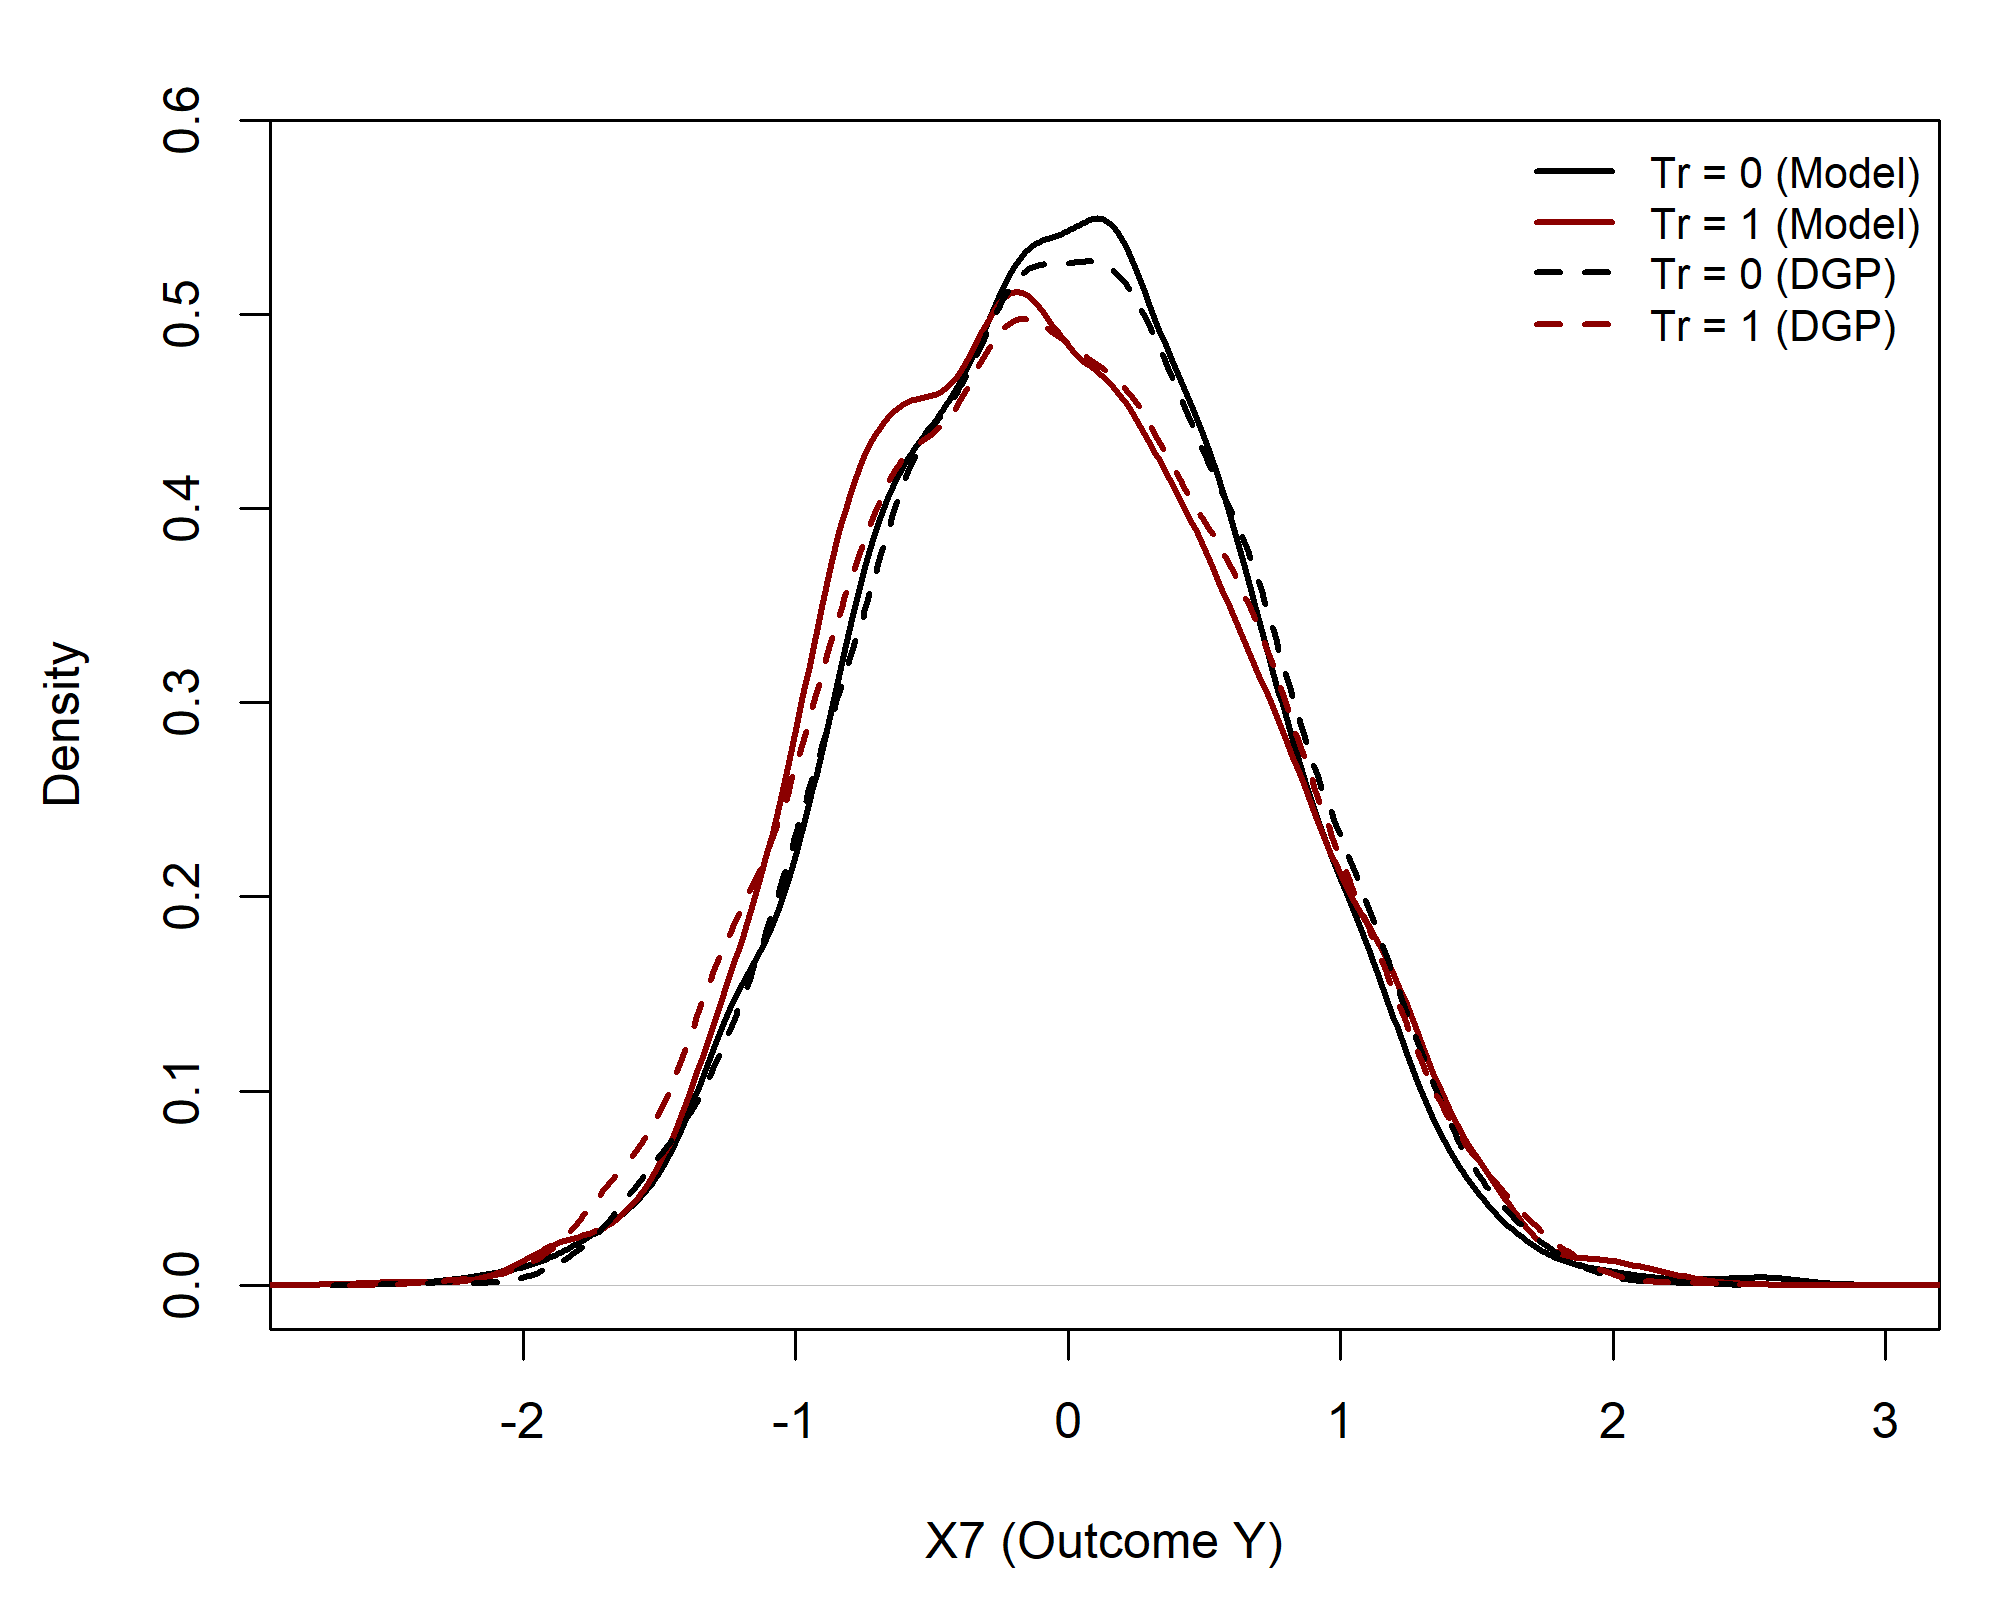
\includegraphics[width=0.45\textwidth]{img/results/observ_scenario3_X7_treatment_densities.png}
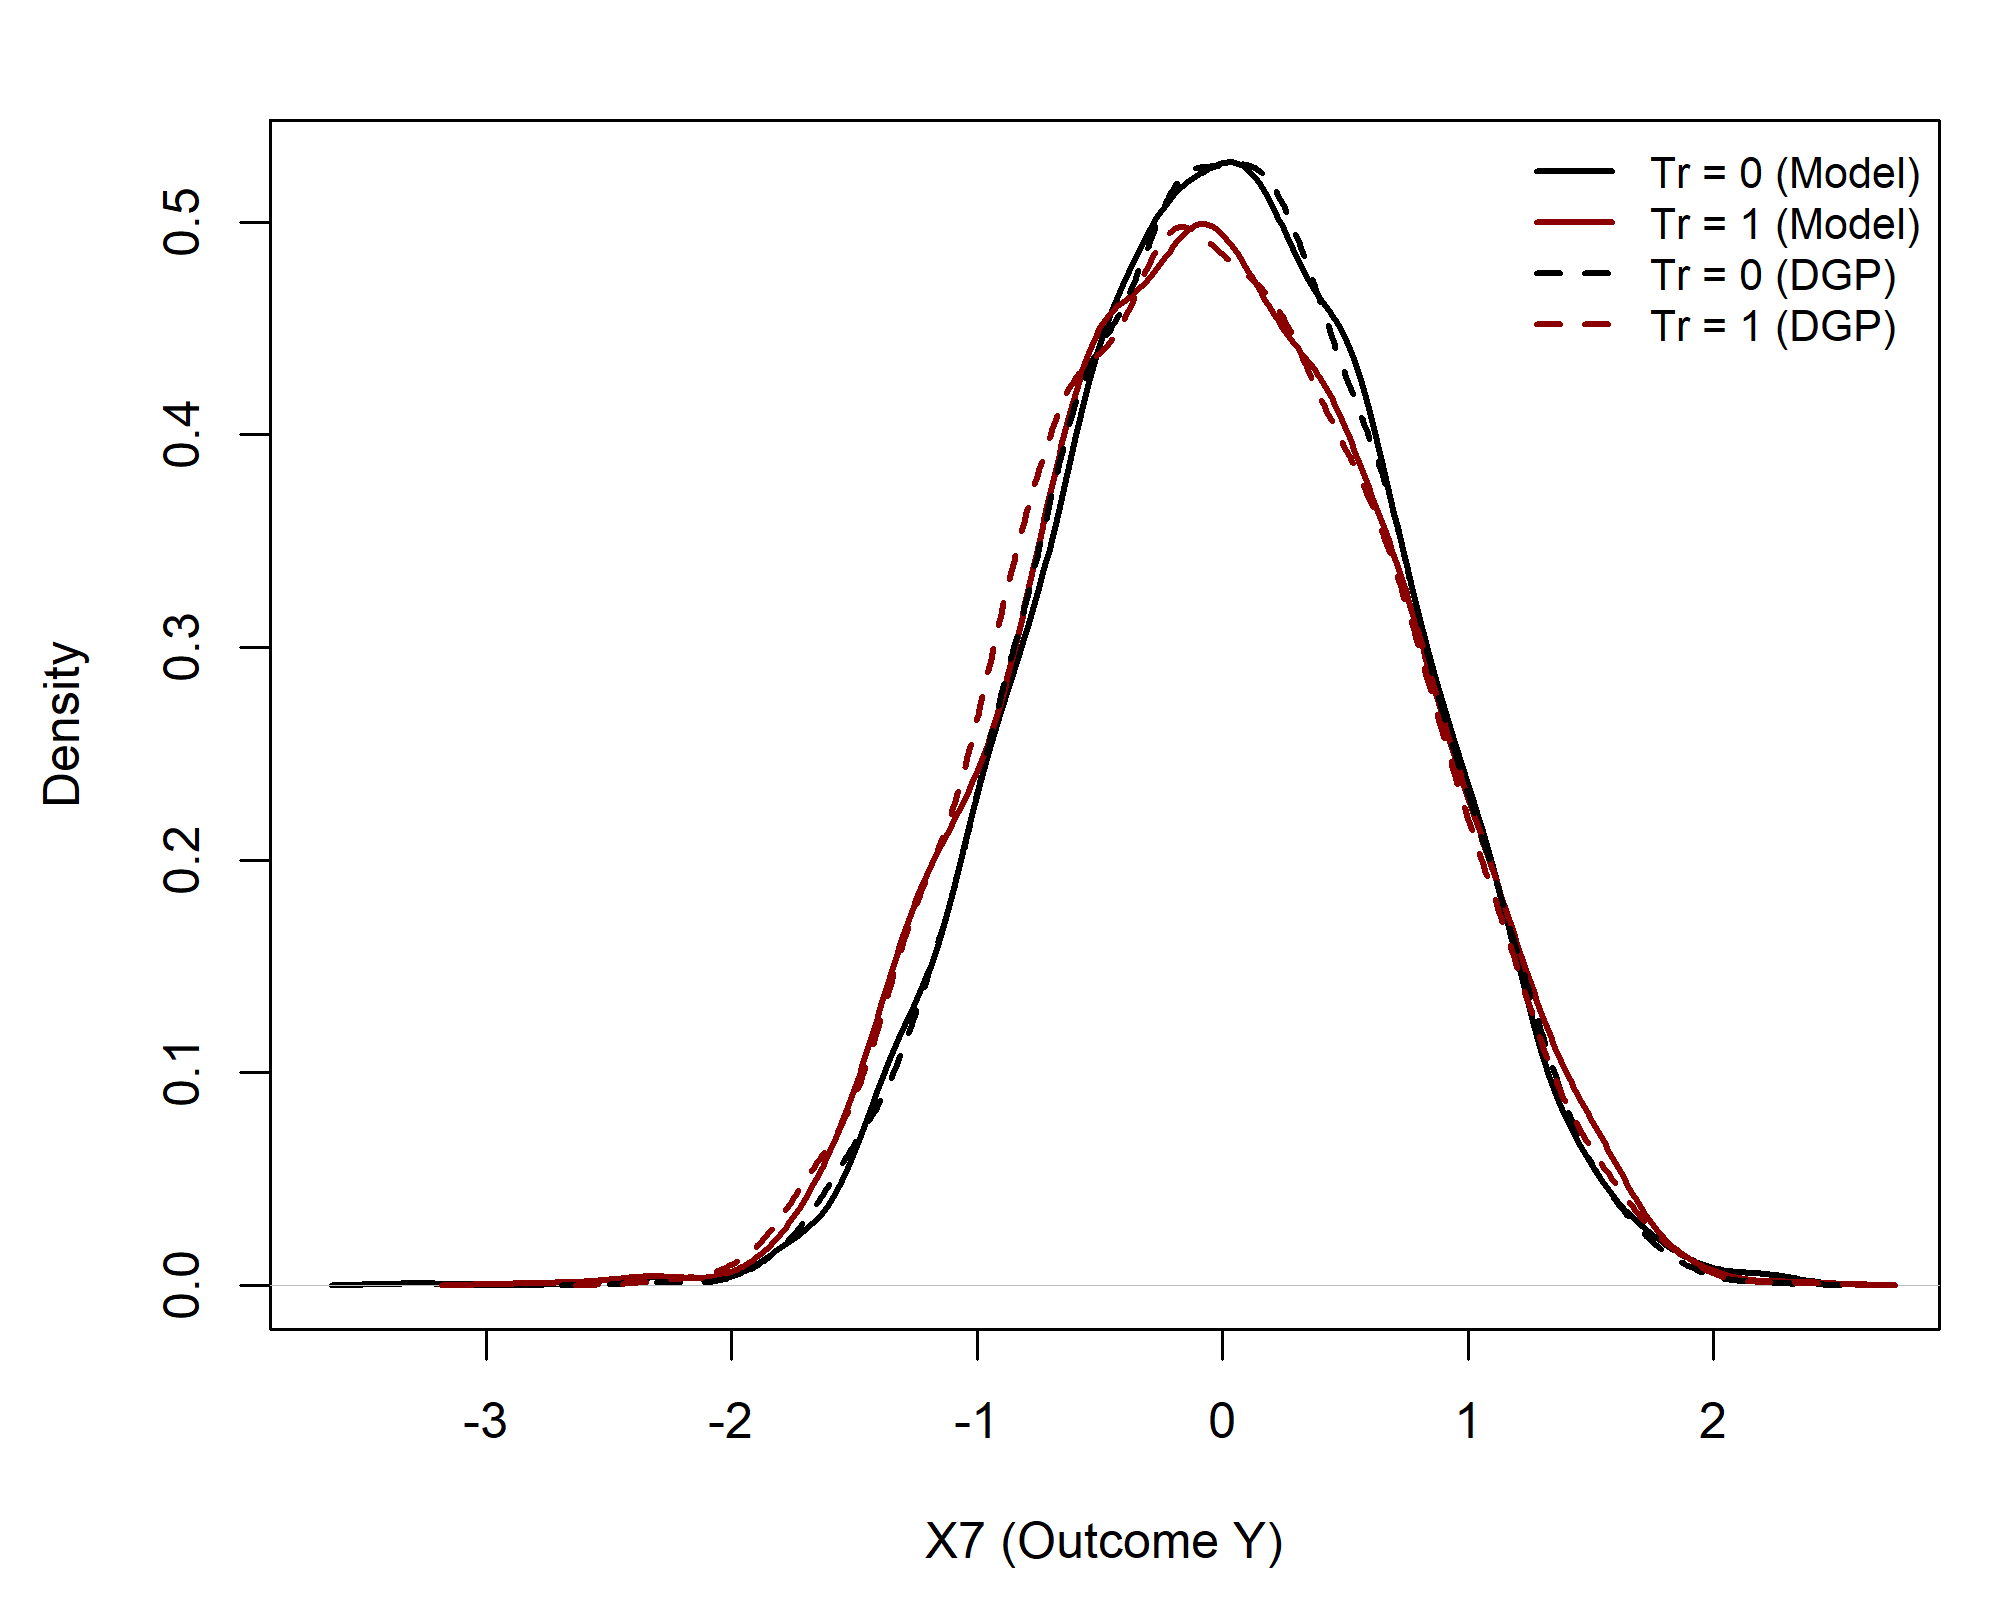
\includegraphics[width=0.45\textwidth]{img/results/rct_scenario3_X7_treatment_densities.png}
\caption{Distributions of the outcome variable (X7) under treatment and control interventions for scenario (3), without direct treatment effect but including interaction effects. This plot is a higher resolution view of the X7 panels (Do $X4=0$) and (Do $X4=1$) from Figure \ref{fig:scenario3_sampling_distributions_vertical}. Left: Observational; Right: RCT setting.}
\label{fig:scenario3_outcome_distributions}
\end{figure}




\begin{figure}[htbp]
\centering
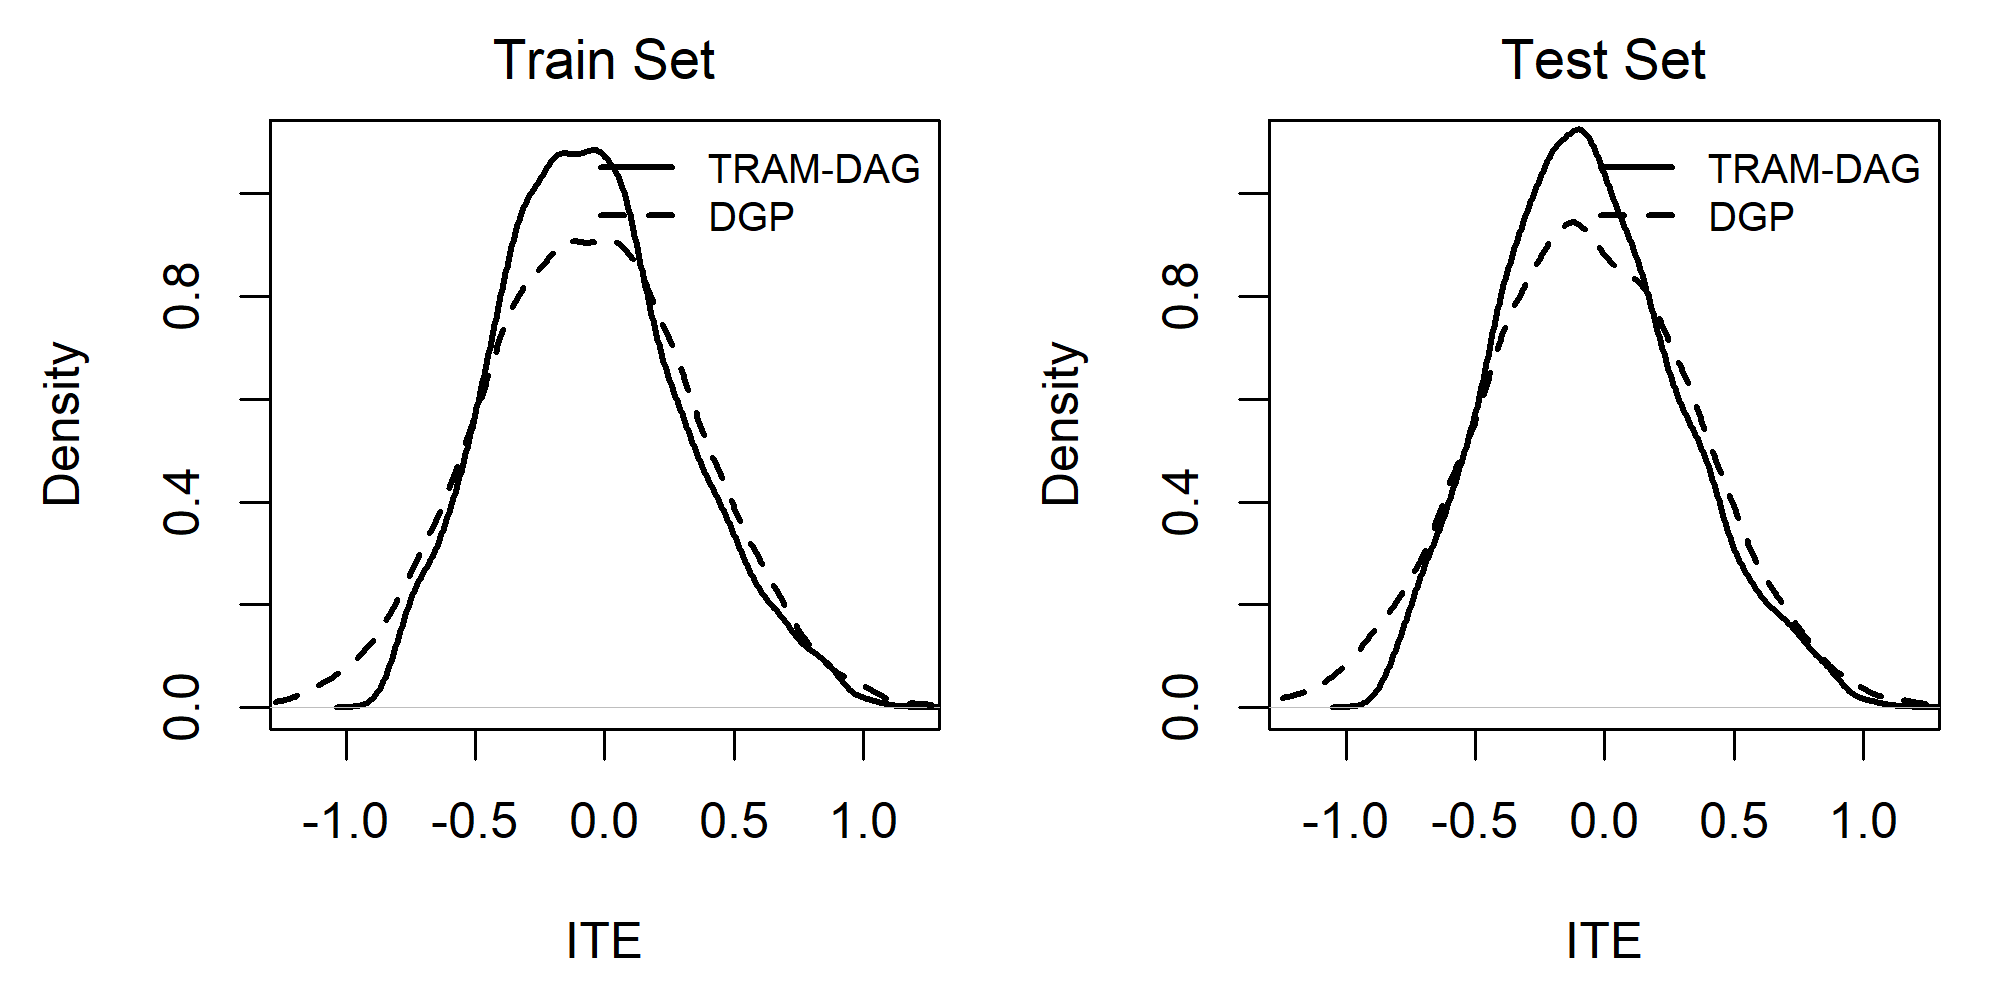
\includegraphics[width=0.45\textwidth]{img/results/observ_scenario3_ITE_densities_train_test.png}
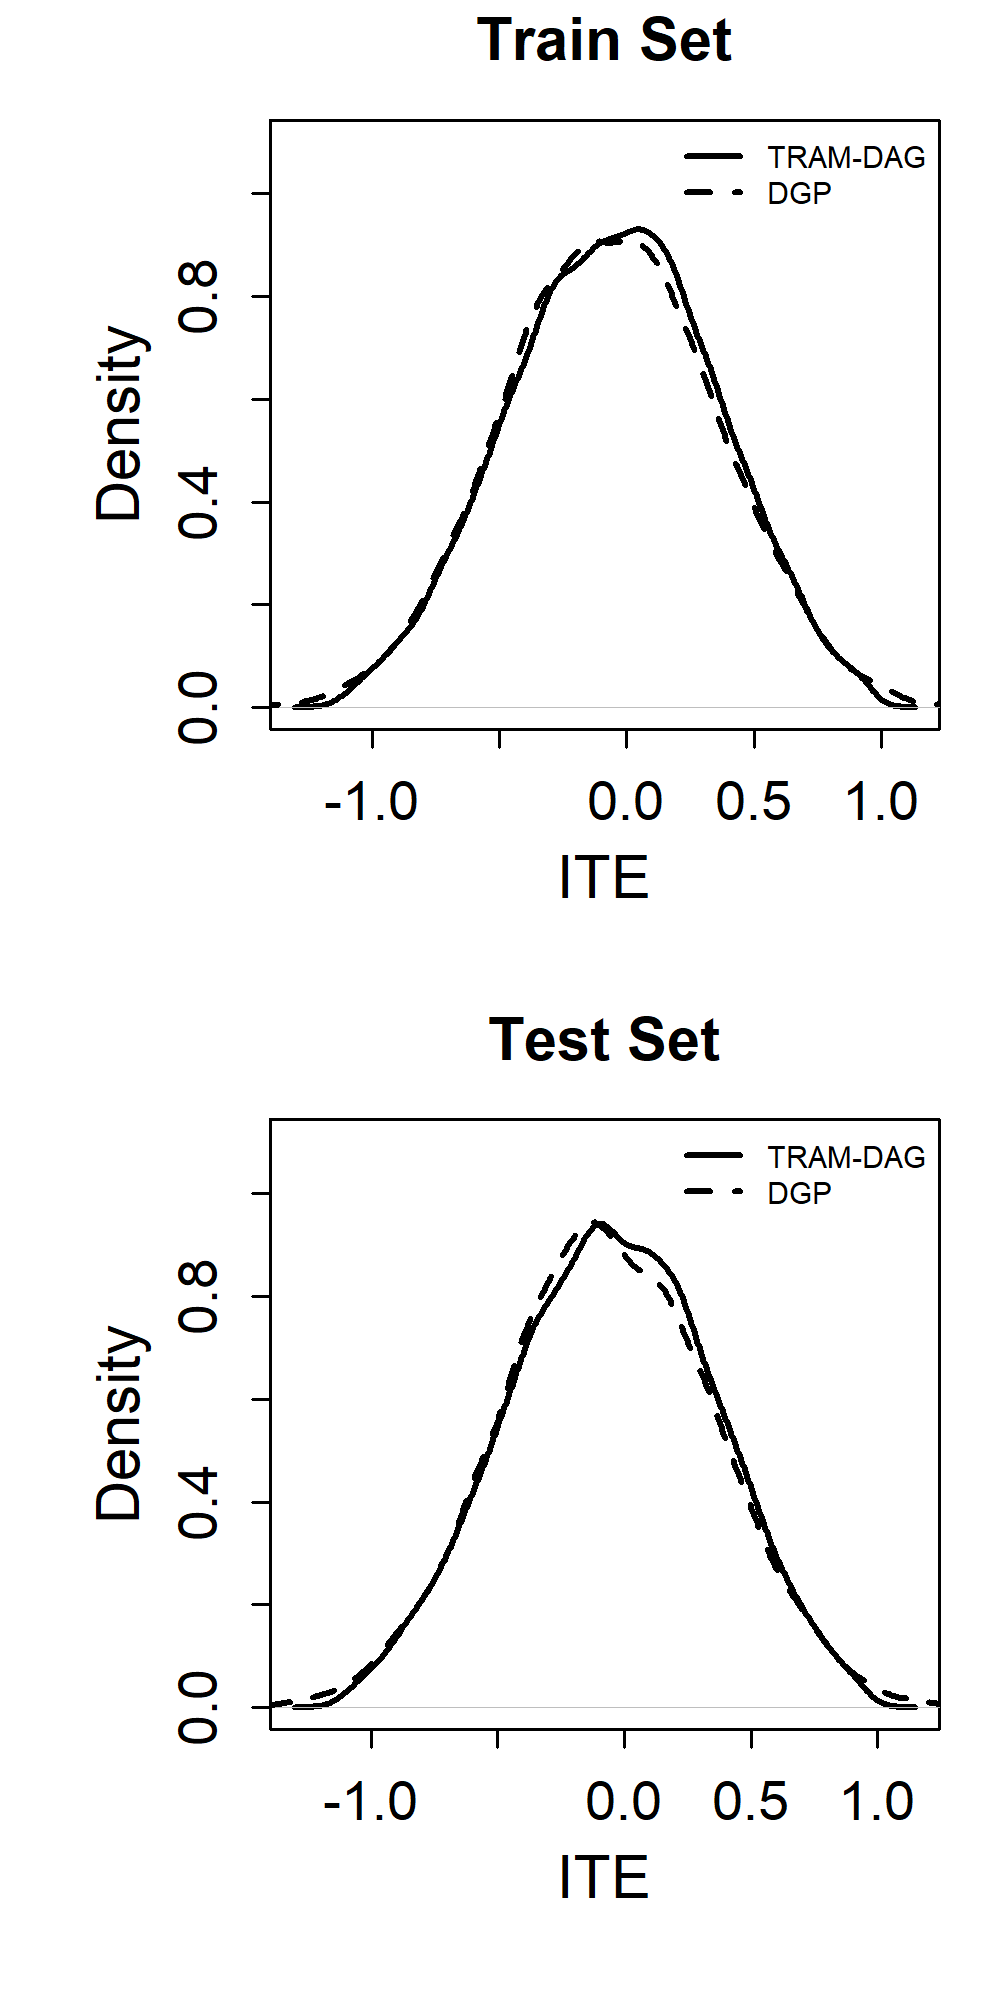
\includegraphics[width=0.45\textwidth]{img/results/rct_scenario3_ITE_densities_train_test.png}
\caption{Densities of estimated ITEs compared to the true ITEs in the training and test datasets for scenario (3), without direct treatment effect but including interaction effects. Left: Observational; right: RCT setting.}
\label{fig:scenario3_ite_densities_train_test}
\end{figure}






\begin{figure}[htbp]
\centering
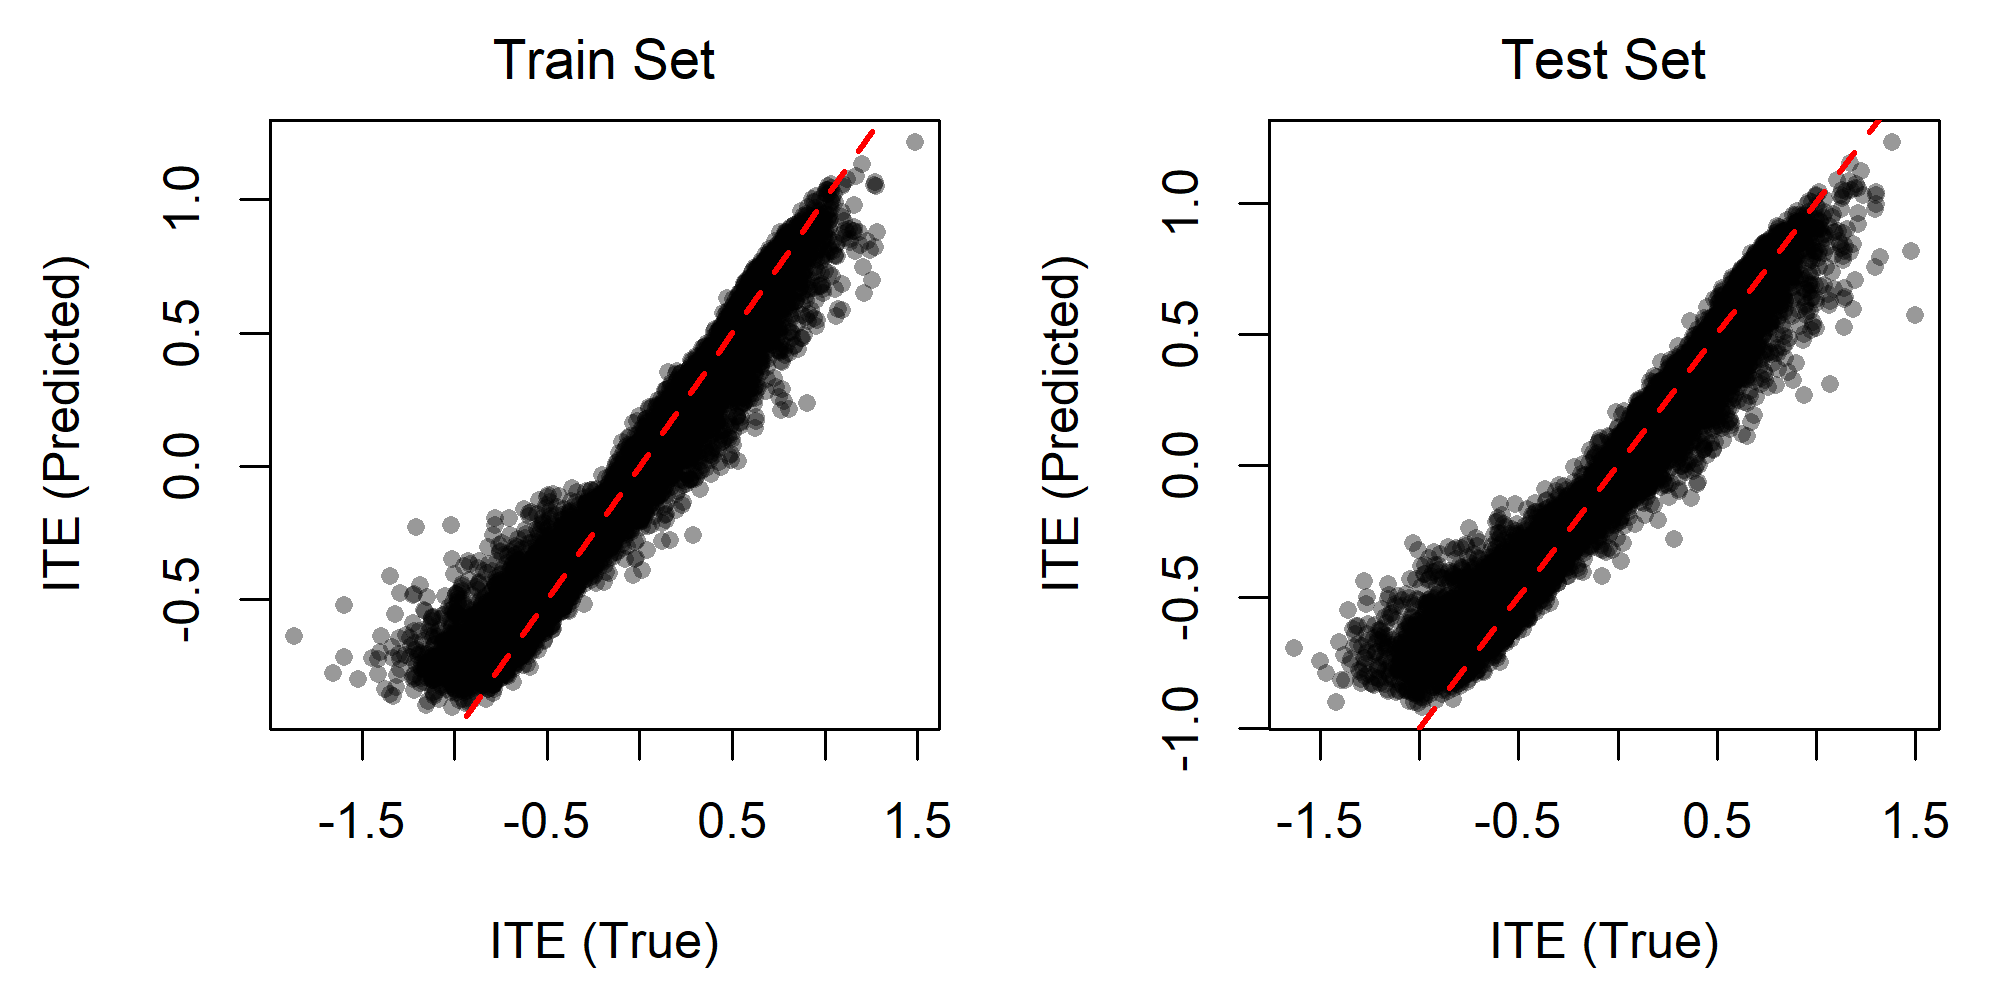
\includegraphics[width=0.45\textwidth]{img/results/observ_scenario3_ITE_scatter_train_test.png}
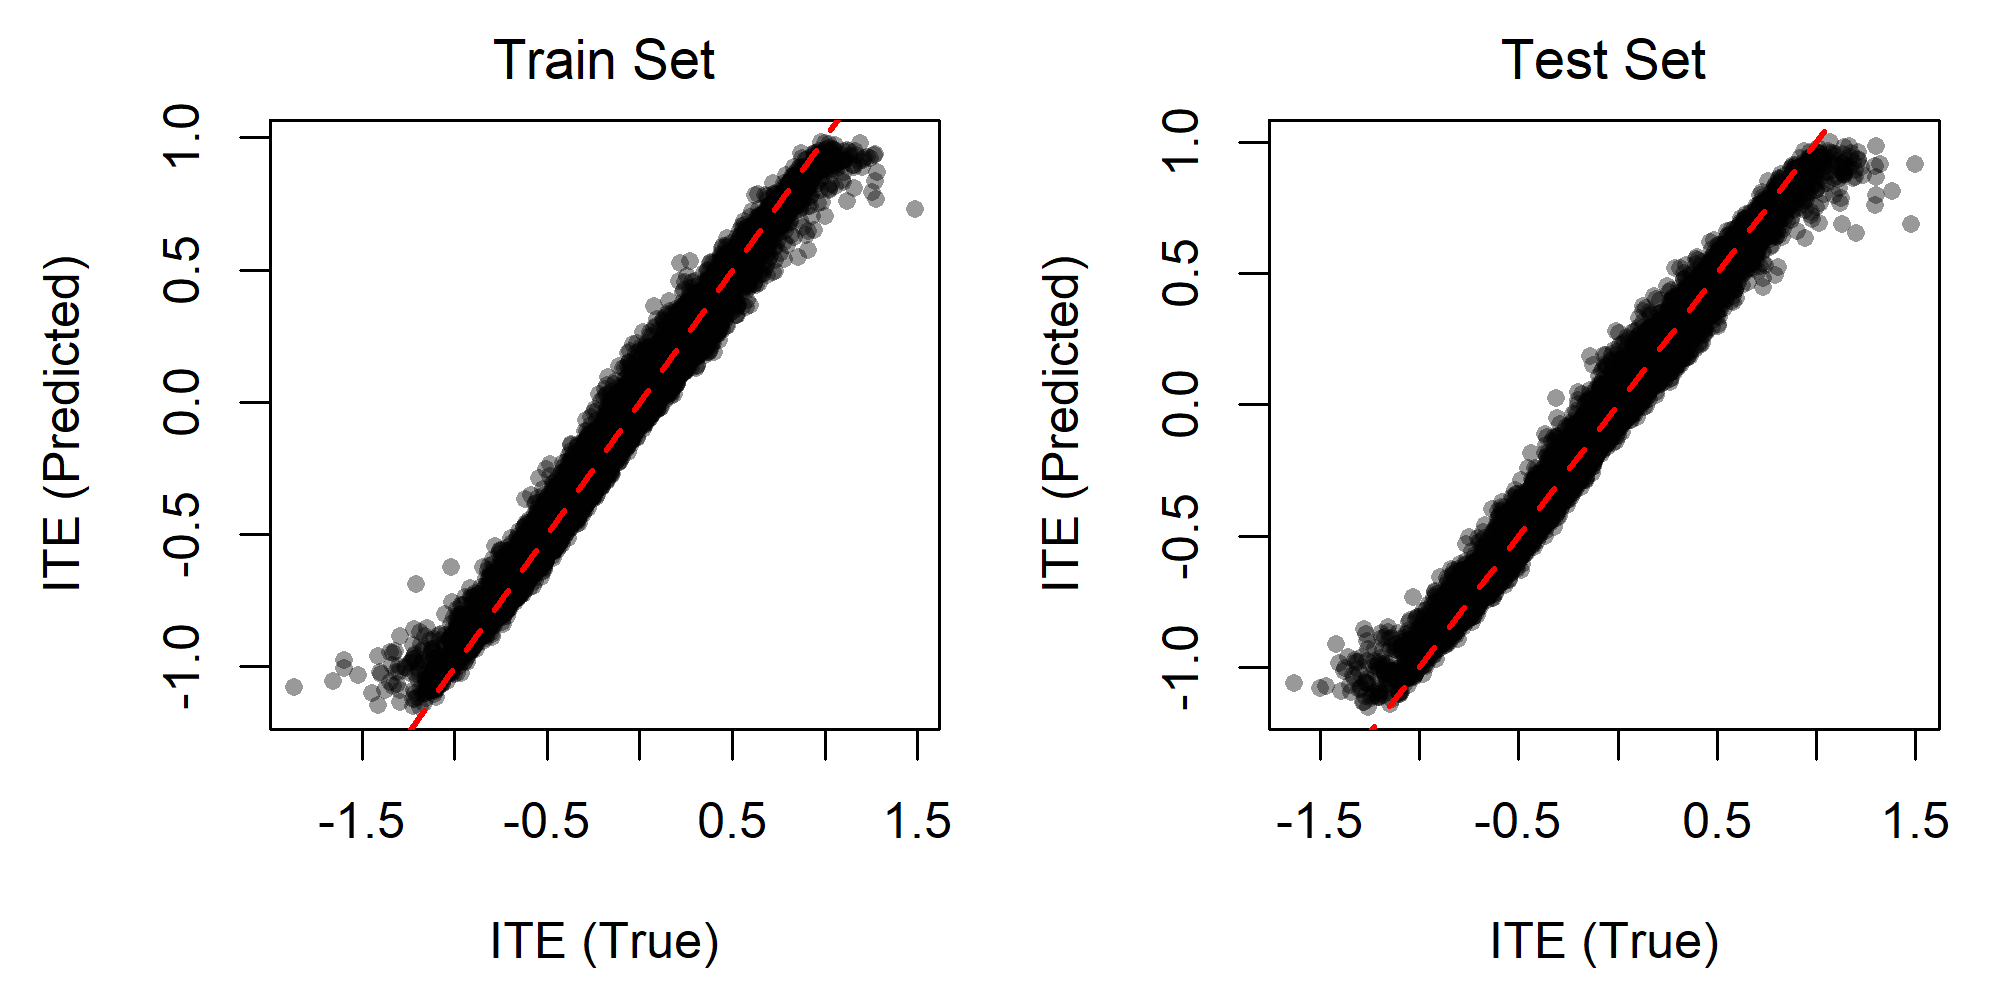
\includegraphics[width=0.45\textwidth]{img/results/rct_scenario3_ITE_scatter_train_test.png}
\caption{Scatterplots of estimated ITEs compared to the true ITEs in the training and test datasets for scenario (3), without direct treatment effect but including interaction effects. Left: Observational; right: RCT setting.}
\label{fig:scenario3_ite_scatter_train_test}
\end{figure}




\begin{figure}[htbp]
\centering
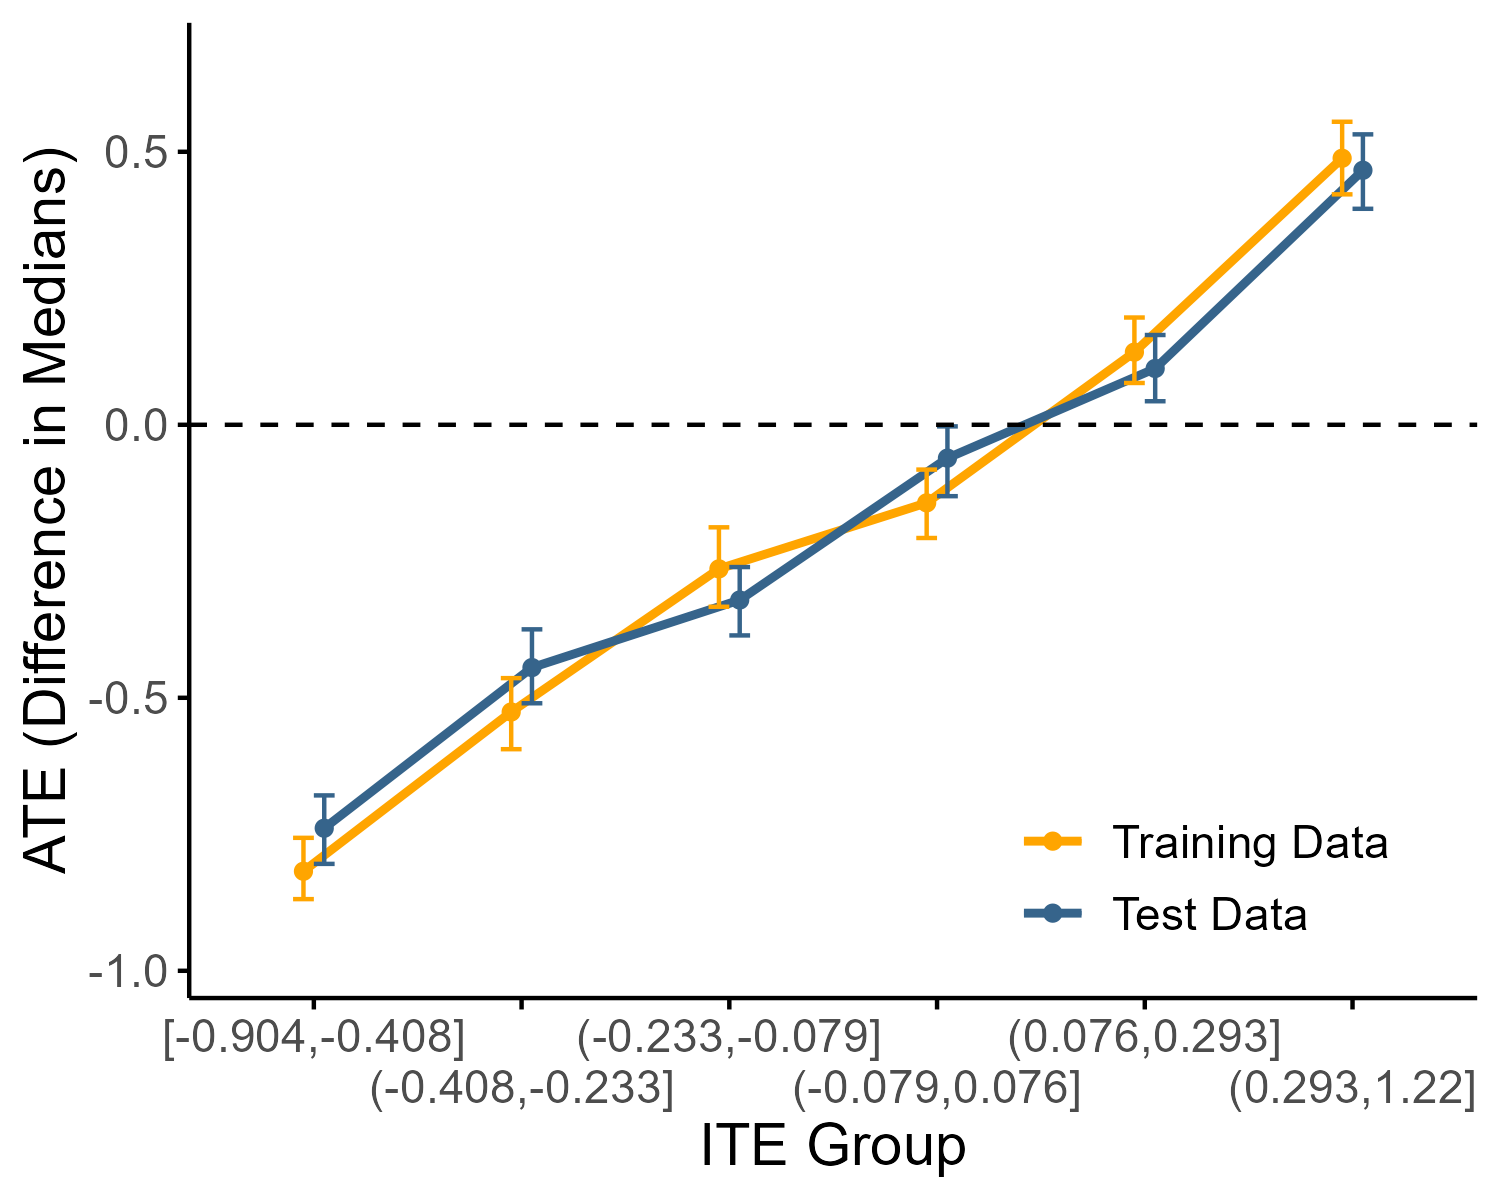
\includegraphics[width=0.45\textwidth]{img/results/observ_scenario3_ITE_cATE.png}
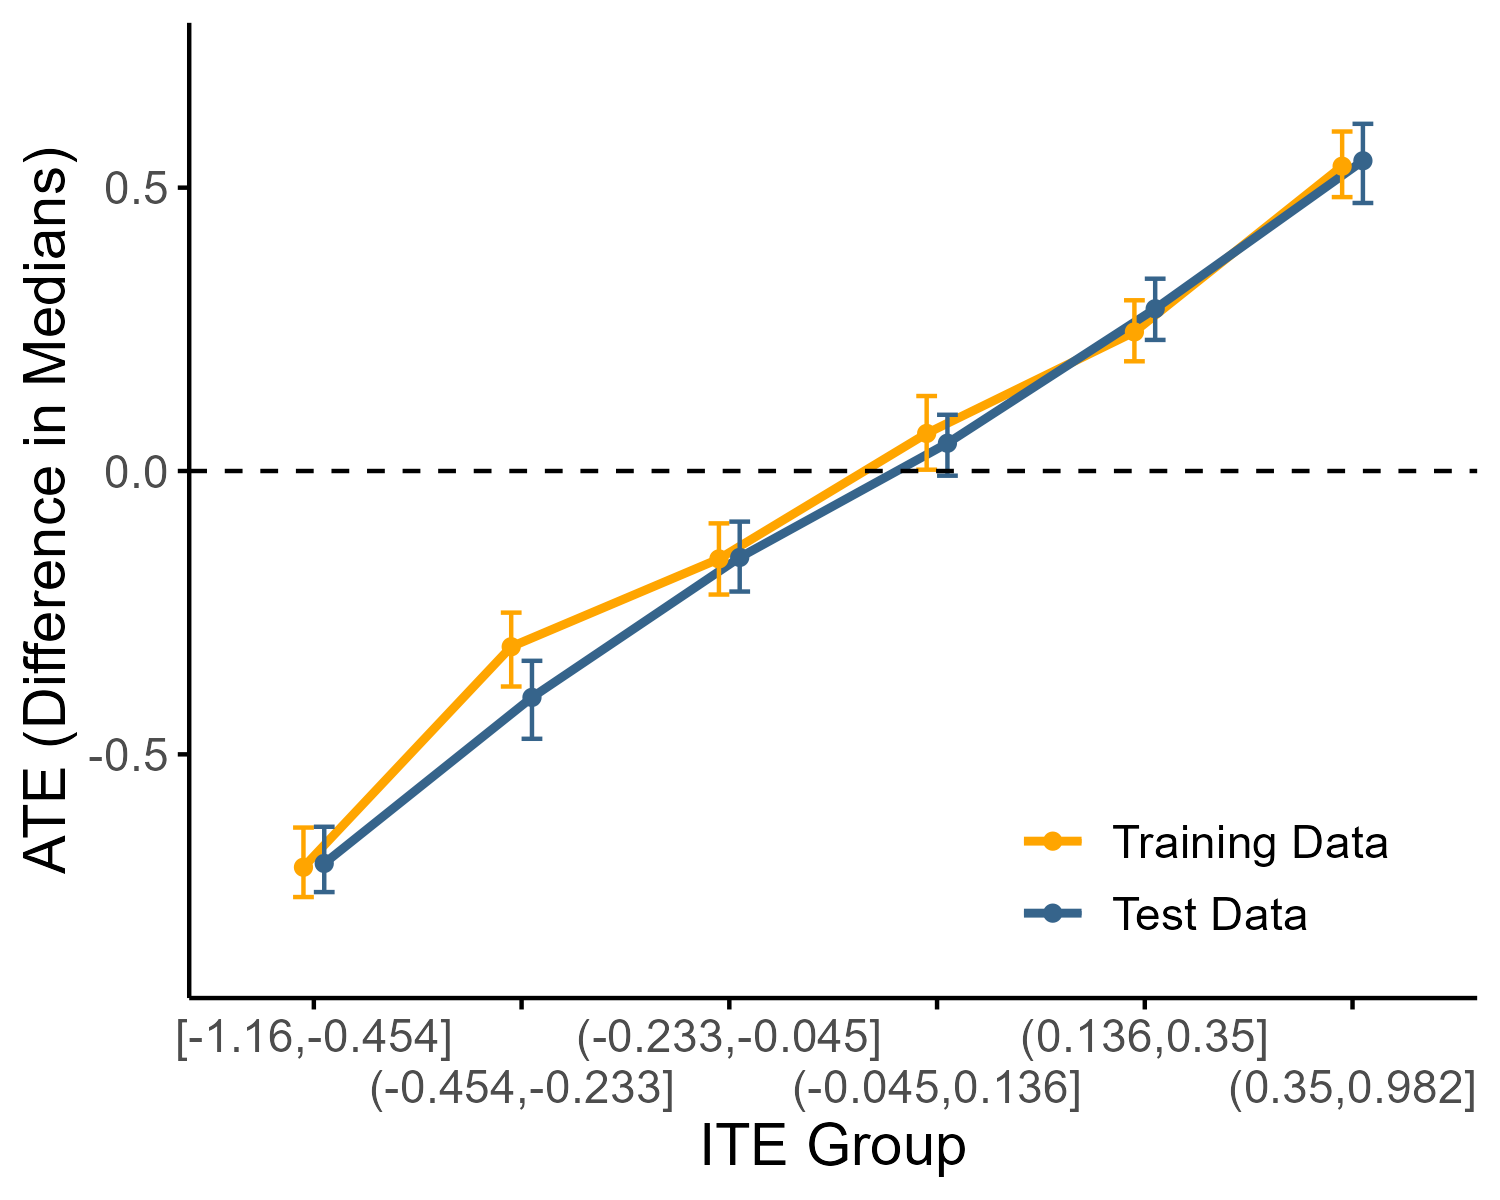
\includegraphics[width=0.45\textwidth]{img/results/rct_scenario3_ITE_cATE.png}
\caption{ITE-ATE plot for scenario (3), without direct treatment effect but including interaction effects. Individuals are grouped into bins according to the estimated ITE and in each bin the ATE is calculated as the difference in medians of the observed outcomes under the treatments. 95\% bootstrap confidence intervals indicate the uncertainty. Left: Observational; right: RCT setting.}
\label{fig:scenario3_ite_cATE}
\end{figure}


